%!!!!!!!!!!!!!!!!!!!!!!!!!!!!!!!!!!!!!!!!!!!!!!!!!!!!!!!!!!!!!!!!!!!!!!!!!!!!!!
%!NOTE: This example file has been prepared according to the University of
%!      Hawaii Style & Policy Manual for Theses and Dissertations dated
%!      "Revised September 2010". If you have one with a later date, you may
%!      need to make revisions to this document as well. In any event, making
%!      sure your thesis complies with Graduate Education guidelines is
%!      ultimately your responsibility. Caveat LaTeXtor. :)
%!!!!!!!!!!!!!!!!!!!!!!!!!!!!!!!!!!!!!!!!!!!!!!!!!!!!!!!!!!!!!!!!!!!!!!!!!!!!!!

%% The options are (you can only choose one from each group):
%%
%% 10pt, 11pt, 12pt: chooses the point size for the document. "11pt" is the
%%                   default.
%%
%% oneside, twoside: whether you want your document onesided or twosided. Note
%%                   that twosided is not guaranteed to work, and style
%%                   guidelines prohibit double sided printouts on final
%%                   copy. "oneside" is the default.
%%
%% draft, final: when printing drafts you can save a lot of paper by using the
%%               "draft" option. It switches to single spacing, displays overful
%%               hboxes with a black box, prints a version number on title page
%%               and omits signature page. Of course for the final copy make
%%               sure to use the "final" option! "final" is the default.
%%
%% thesis, dissertation: switches between the style for a master's thesis and a
%%                       Ph.D. dissertation. The differences are fairly minor
%%                       and limited to the front matter. "thesis" is the
%%                       default.
%%
%% actual, proposal: switches between actual document and proposal mode. In
%%                   proposal mode: the title page is simplified and the
%%                   version number is always printed.
%%
%%% Load the new uhthesis document class
\documentclass[11pt, dissertation]{uhthesis}

%%% Load some useful packages:
%% New LaTeX2e graphics support
\usepackage{graphicx}
%% Package to linebreak URLs in a sane manner.
\usepackage{url}

\usepackage{hyperref}

% Allows us to position our tables inline. https://stackoverflow.com/a/1674386
\usepackage{float}
\restylefloat{table}

\usepackage{amsmath}
\usepackage{tabularx}
\usepackage{ltablex}
\usepackage{booktabs}
\usepackage{array}
\usepackage{cleveref}
\usepackage{bm}
\usepackage{subfig}
\usepackage{appendix}
\usepackage{tcolorbox}
\usepackage{listings}

\lstset{
basicstyle=\small\ttfamily,
columns=flexible,
breaklines=true
}

%%% Declarations for Front Matter. Capitalize all of these values
%%% "normally". This allows the document class to format them properly.
%% Full title of thesis or dissertation, capitalized like a title should be.
\title{Laha: a Framework for Adaptive Optimization of Distributed Sensor Frameworks}
%% Your name, capitalized normally. Do not include any titles like Dr.
\author{Anthony J. Christe}
%% Month in which you intend to receive your degree (i.e. graduation).
%% Presumably this will be one of: May, August, or December.
\degreemonth{May}
%% Year of expected graduation.
\degreeyear{2020}
%% Type of degree to be conferred.
\degree{Doctor of Philosophy}
%% This is the chairperson of your committee. Do not use titles like Dr.
\chair{Philip Johnson}
%% The other members of your committee, seperated by "\\". Again, no titles,
%% and it is customary to list the outside committee member (if you have one)
%% last.
\othermembers{Lipyeow Lim\\
Dan Suthers\\
Peter Sadowski\\
Milton Garces}
%% The field in which you are obtaining your degree, capitalized normally.
\field{Computer Science}
%% If your discipline allows subfields, you can add it here. Note that this
%% is strictly controlled, so consult the Style & Policy guide before adding
%% a subfield.
%\subfield{Bioinformatics}
%% 4-6 optional keywords/phrases for use in indexing or as search terms
\keywords{distributed, sensors, management, adaptive, optimizing, predictive}
%% The version number of your document. Consistent use of this will enable you
%% to tell old drafts from new ones. Final actual documents omit this
%% automatically so you can use it without fear of submission problems at the
%% end. If you do not define this parameter, it defaults to "1.0.0".
\versionnum{1.0}

%%% End of preamble

\begin{document}
\maketitle

\begin{frontmatter}

%%% Note, there is no longer a signature page included in the document, it
%%% has been replaced by Form IV

%%% Create the copyright page (optional)
\copyrightpage

%%% Bring in the dedication page from external file (optional)
\begin{dedication}
    \null\vfil
    {\large
    \begin{center}
        To my father, Raymond, if only you could see me now. To my wife, Christine, thank you for your everlasting support. To my mother, Sharon, I told you I would graduate eventually.
    \end{center}}
    \vfil\null
\end{dedication}


%%% Bring in the acknowledgments section from external file (optional)
\begin{acknowledgments}
    I would like to thank my committee for providing me the opportunity to perform the research outlined in this dissertation. I would like to thank Philip for the endless hours of editing, wordsmithing, and inspiration. I would like to thank Milton for the invaluable lessons on navigating the Ph.D. process. Without a dedicated team of support, this dissertation would have never come to fruition.
\end{acknowledgments}


%%% Bring in the abstract section from external file
\begin{abstract}
	Distributed Sensor Networks (DSNs) face a myriad of technical challenges. This dissertation examines two important DSN challenges.

	One problem is converting ``primitive" sensor data into actionable products and insights. For example, a DSN for power quality (PQ) might gather primitive data in the form of raw voltage waveforms and produce actionable insights in the form of the ability to predict when PQ events are going to occur by observing cyclical data. For another example, a DSN for infrasound might gather primitive data in the form of microphone counts and produce actionable insight in the form of determining what, when, and where the signal came from. To make progress towards this problem, DSNs typically implement one or more of the following strategies: detecting signals in the primitive data (deciding if something is there), classification of signals from primitive data (deciding what is there), and localization of signals (when and where did the signals come from). Further, DSNs make progress towards this problem by forming relationships between primitive data by finding correlations between spatial attributes, temporal attributes, and by associating metadata with primitive data to provide contextual information not collected by the DSN. These strategies can be employed recursively. As an example, the result of aggregating typed primitive data provides a new higher level of typed data which contains more context than the data from which is was derived from. This new typed data can itself be aggregated into new, higher level types and also participate in relationships.

	A second important challenge is managing data volume. Most DSNs produce large amounts of (increasingly multimodal) primitive data, of which only a tiny fraction (the signals) is actually interesting and useful. The DSN can utilize one of two strategies: keep all of the information and primitive data forever, or employ some sort of strategy for systematically discarding (hopefully uninteresting and not useful) data. As sensor networks scale in size, the first strategy becomes unfeasible. Therefore, DSNs must find and implement a strategy for managing large amounts of sensor data. The difficult part is finding an effective and efficient strategy deciding what data is interesting and must be kept and what data to discard.

	This dissertation investigates the design, implementation, and evaluation of the Laha framework, which provides new insight into both of these problems. First, the Laha framework provides a multi-leveled representation for structuring and processing DSN data. The structure and processing at each level is designed with the explicit goal of turning low-level data into actionable insights. Second, each level in the framework implements a ``time-to-live" (TTL) strategy for data within the level. This strategy states that data must either ``progress" upwards through the levels towards more abstract, useful representations within a fixed time window, or be discarded and lost forever. The TTL strategy is useful because when implemented, it allows DSN designers to calculate upper bounds on data storage at each level of the framework and supports graceful degradation of DSN performance.

	There are several smaller, but still important problems that exist within the context of these two larger problems. Examples of the smaller problems that Laha hopes to overcome in transit to the larger goals include optimization of triggering, detection, and classification, building a model of sensing field topology, optimizing sensor energy use, optimizing bandwidth, and providing predictive analytics for DSNs.

	Laha provides four contributions to the area of DSNs. First, the Laha design, a novel abstract distributed sensor network that provides useful properties relating to data management. Second, an evaluation of the Laha abstract framework through the deployment of two Laha-compliant reference implementations, validated data collection, and several experiments that are used to either confirm or deny the benefits touted by Laha. Third, two Laha-compliant reference implementations, OPQ and Lokahi, which can be used to form DSNs for the collection of distributed power quality signals and the distributed collection of infrasound signals. Fourth, a set of implications for modern distributed sensor networks as a result of the evaluation of Laha.

	The major claim of this dissertation is that the Laha Framework provides a generally useful representation for real-time high-volume DSNs that address several major issues that modern DSNs face.
\end{abstract}


%%% Generate Table of contents
\tableofcontents

%%% Generate list of tables
\listoftables

%%% Generate list of figures
\listoffigures

\end{frontmatter}

%\normalsize
%%% Bring in the body of the thesis from external file
\chapter{Introduction}
Distributed sensor networks (DSNs) consist of any number of sensors that collect and sense information about the physical environment around them. The sensors that make up these networks can either be homogeneous or heterogeneous. Distributed sensor networks are dynamic in that sensors can be added or removed from the network at any time. DSNs also increasingly include mobile sensors as well. With the onset of the Internet of Things (IoT), its easier than ever to build and deploy distributed sensor networks. Further, mobile devices, such as mobile phones, are seeing increased usage as intelligent sensing agents.

Distributed sensor network (DSN) optimization is a broad topic with many different facets to consider. Much of the literature on the topic focuses on optimizing data flow between sensors as data flows from sensor to sensor and eventually to a sink. 

The focus of this dissertation however, is to deal with the challenges of a specific subset of DSNs. That subset is DSNs where data always flows directly from each sensor in the network to sink nodes, thus, eliminating the need to worry about intra-sensor communication, networking, and routing. 

There are a broad range of technical challenges beyond the data sink. The introduction of the Internet of Things (IoT) has created an explosion of internet connected devices that sense a massive number of attributes about the physical world surrounding them. An increase in sensors has created an increase in multimodal data generation with the inverse problem of creating a decrease in the signal-to-noise ratio, making it more difficult to identify and classify signals of interest. Multimodal data provides challenges for analysis algorithms because each sensor may be streaming multiple physical features that need to be analyzed and dealt with independently and dependently. As the densities of sensors increase, analysis must be able to work with missing data, incorrect data, incomplete data, and data coming from a heterogeneous mix of hardware and sensor configurations. Further, we can no longer assume that sensors are static in time and location as mobile sensors are quickly becoming more prevalent, making analysis trickier. All of these issues require an increase in storage and computational resources. Therefore, we must find approaches to deal with sensor data to lessen these hurdles.

As DSNs scale, available storage must be balanced with the amount of data being retained. Further, once data is collected, we need strategies for turning sensor data into actionable data and insights. This generally involves detecting and classifying signals of interest. It's these last two important DSN challenges that are the focus of this dissertation.

\section{Converting Sensor Data into Actionable Insights}\label{sec:converting-sensor-data-into-actionable-insights}
Data collected from sensors is often a sampled payload of data points representing some feature in the physical world. As examples, weather stations produce sampled features relating to temperature, wind speed, and humidity, power meters produce a metric of total electricity consumed, power quality sensors produce sampled data points which include voltage, frequency, and THD, and infrasound networks produce sampled data which represent audio waveforms.

These features by themselves, while interesting, do not provide any context as to if there is a signal, what the signal is, when and where the signal came from, or what caused the signal in the first place. Detection and classification algorithms are used to attempt to extract some of these properties. Primitive data is aggregated and compared to other primitive data to find correlations in both time and space. Data is compared to historic data in an attempt to find patterns or other similarities. This type of data is more interesting in that we might learn more about a signal using these techniques, but they still don't provide actionable insights or causality information. Further, the problem of providing actionable insights is highly dependent on the sensing domain. Depending on other available sources of data, providing data fusion and context from outside of the DSN can be difficult.

Evaluation of converting sensor data into actionable insights is provided in Section~\ref{subsec:evaluation-of-converting-primitive-data-into-actionable-insights}. Results of converting sensor data into actionable insights is provided in Section~\ref{sec:results-of-converting-primitie-data-into-actional-insights}.

\section{Big Data Management in DSNs}\label{sec:big-data-management-in-dsns}
Big Data is generally defined by the four V's; volume, velocity, variety, and value. These characteristics can be observed in many of the DSNs that exist and are being created today.

That is, distributed sensor networks create a large volume of data due to the abundance of IoT and mobile devices that make up DSNs. As communication infrastructures improve and hardware becomes smaller, smarter and more energy efficient, sensors are able to send and transfer larger amounts of data. The ease of building and deploying sensors in DSNs means that more sensors can be produced much more cheaply allowing for more sensors to be used within a DSN, increasing coverage, but also increasing the volume of data.

Distributed sensor networks create a variety of data with different formats and data quality issues. Distributed sensor networks can produce data at high velocity. These characteristics of data produced from distributed sensor networks create a need for efficient architectures and specific algorithms designed for working with Big Data.

Further, sensor networks are often constrained in both computing power and available energy sources. This forces us to find comprises between data collection, onboard sensor processing, sensor communication, and network coordination.

As DSNs scale, the amount of data a DSN must store and process increases. At certain scales, DSNs simply can not store and process all of the primitive data that sensors are producing or process and store aggregate data products that detection and analysis routines produce. Designers of a DSN can either choose to collect and keep all data forever (from raw data to generated products), or they can implement strategies for systematically discarding (hopefully) non-interesting data. If the first option is chosen, then there is no risk of accidentally discarding signals of interest and data can be reanalyzed when analysis algorithms change or are tweaked. However, storage and analysis of such amounts of data can cause system degradation or even be unfeasible. If the second option is chosen, processes must be put in place that attempt to only store ``interesting" data and discard sensor noise.  The second option runs the risk of discarding important data and old data can not be reanalyzed under this approach. However, this approach provides the benefits of providing predictable data storage requirements that can be tuned and optimized for a particular domain and DSN.

Evaluation of big data management in DSNs is provided in Section~\ref{subsec:eval-big-data}. Results of big data management in DSNs is provided in Section~\ref{sec:dsn-system-requirements}.

\section{Traditional Approaches to DSN Optimization}\label{sec:traditional-approaches-to-dsn-optimization}
Much of the literature focuses on the reduction of bandwidth and communication between sensors nodes and between sensor nodes and the sink. This is mainly performed as a means of sensor energy requirements allowing sensing to stay online longer or focus their energy usage for sensing or edge level computing. Anastasi et al\cite{anastasi_energy_2009} provide a really nice literature review on techniques for energy conservation in wireless sensor networks. Many of these approaches utilize optimized triggering\cite{alippi_adaptive_2010} or exploitation of topology knowledge\cite{warrier2007much} to minimize sensor communications and save sensor energy.  General approaches to Big Data management include compression\cite{tang2004compression} or storage systems where the goal is to have a distributed file system and move data close to where it is being processed, such as the Hadoop Distributed File System\cite{warrier2007much}. Other systems such as NiFi\cite{hughes2016survey} provide a nice interface for ingestion and movement of data between Big Data tools while also providing data provenance, but do not go far enough in focusing on data reduction and graceful degradation. Carney et al.\cite{carney2002monitoring} discuss how monitoring applications require management and clean up of stale sensor data. Much of the literature on topology management is written to decrease sensor energy requirements by exploiting the density of sensors within a sensing field topology. For example, the ASCENT\cite{cerpa2004ascent} framework provides adaptive self configuring sensors that exploit topology denseness to decrease sensor energy usage. Several other frameworks have been designed with the same goal of reducing energy usage by exploiting topology\cite{schurgers2002stem,schurgers2002topology}.

\section{Laha: An Abstract Framework for Adaptively Optimizing DSNs}\label{sec:laha:-an-abstract-framework-for-adaptively-optimizing-dsns}
I have designed an abstract distributed sensor network framework, Laha, that adaptively optimizes data storage using a tiered TTL approach and makes strides towards providing actionable data by providing a mechanism in which typed aggregated data is continually refined to the point of being of becoming actionable. % triggering, collection, detection, classification, sensor device power requirements, and bandwidth. 

The Laha data model can be conceptualized as a multilevel pyramid (see Figure~\ref{laha-abstract-overview}). Laha Actors act on the data model to move data upward through the levels and to apply optimizations downward through the levels. Many of these optimization techniques were developed independently. Laha provides a conceptual framework that enables them to work together.

The lowest level stores all recently received raw sensor data. This data expires and is automatically removed within a limited period of time (for example, 1 hour) unless the data is found to be interesting, and is thus propagated upwards to the next level of the hierarchy.  Higher levels of the data hierarchy organize data in the same way, however each level adds context to the examined signal or signals. Context includes classifications, locality metrics, temporal metrics, or similarities to current or prior signals of interest. The highest level of the hierarchy, Phenomena, represents predictive capabilities of the sensor network which are then used to optimize and tune the lower levels. The Phenomena also form the basis for providing actionable insights. 

A high level summary of the Laha abstract framework is provided as Figure~\ref{laha-abstract-overview} which shows the levels and names of the hierarchy, a brief description of the functions of each level, and Laha's Actors and how they move data upwards (right hand side) and how they apply optimizations downwards (left hand side).

\begin{figure}
	\caption{Laha Conceptual Model Summary}
	\centering
	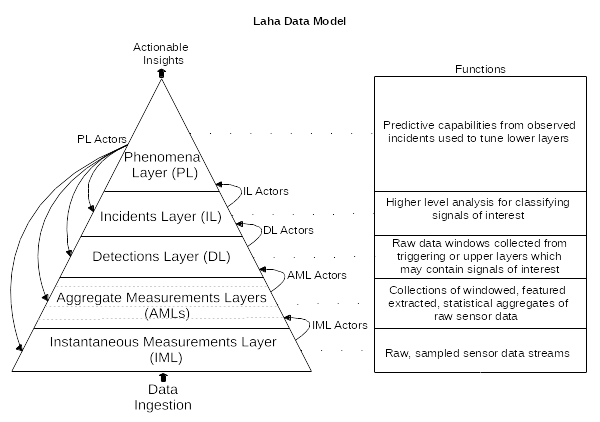
\includegraphics{figures/laha_abstract_overview.png}
	\label{laha-abstract-overview}
\end{figure}

The Laha framework aims to provide two important benefits to DSNs:
\begin{enumerate}
	\item Convert sensor data into actionable data and insights
	\item Provide graceful degradation and metrics on storage requirements for voluminous sensor data
\end{enumerate}

Although not the main focus of this dissertation, Laha provides several tangential benefits in the following DSN problem domains:

\begin{enumerate}
	\item Triggering optimizations
	\item Detection and classification optimizations
	\item Topological optimizations
	\item Sensor energy requirement optimizations
\end{enumerate}

These tangential benefits are provided by Laha Actors that exist within each level of the Laha framework. I don't claim that these techniques are novel, but I do claim that either all or a subset of these techniques are required to enable progress towards the main goals of this framework. To that end, Laha Actors implement several state of the art algorithms present in the literature that address these tertiary problems.

Laha is evaluated by designing and implementing two Laha-compliant reference implementations, OPQMauka and Lokahi. Open Power Quality (OPQ) is a power quality (PQ) network consisting of custom hardware and distributed software services that detect distributed PQ signals such as voltage sags and swells, frequency sags and swells, transients, THD, and other known PQ issues. OPQMauka is a distributed, plugin based middleware component of OPQ that performs higher level analysis, data management, and optimizations of the OPQ services. Lokahi is a distributed infrasound network consisting of mobile iOS and Android devices and multiple cloud based software services whose purpose is to supplement the International Monitoring System (IMS) in detecting large infrasound signals.

The reference implementations are designed and were deployed to test sites at UH Manoa and at the Infrasound Laboratory in Kailua-Kona, Big Island.

Data collected from the PQ network was validated against calibrated reference sensors that have already been installed at the power mains of a subset of buildings on campus. The Office of Energy Management at UH Manoa has given us full access to live and historic PQ data collected at these reference sensors. OPQBoxes were co-located and placed in buildings with the reference sensors so that I can validate that the triggering and raw data streams I receive from the OPQBoxes are in line with what the reference sensors are observing.

Data collected from the infrasound network was also validated against industry standard calibrated BNK infrasound sensors. Further, signals in the infrasound network are known a priori since I am able to control the signals that are generated from our calibrated infrasound source, allowing further validation of received signals.

In order to evaluate the generality of the Laha-framework, two separate Laha-compliant DSNs sensing different domains were designed, distributed, and evaluated. 

The first Laha-compliant DSN is Open Power Quality (OPQ), a distributed DSN that collects and analyzes power quality (PQ) signals. PQ is a measure of the ``goodness" of the power feeding your electronics. The features that this network collects includes voltage, frequency, and THD. From these features, OPQ can classify the following PQ signals: voltage dips/swells, frequency dips/swells, high levels of THD, and transients. Another goal of this network is to detect distributed PQ signals. That is, the same signal detected on multiple sensors to study how PQ signals move through a power grid. This network provides metrics on the number of incidents classified as well as numbers of correct predictions from Phenomena. The number of classified incidents are compared to industry standard PQ monitors co-located with OPQ sensors as a means of evaluating if Laha is capable of supporting the goals of this network.

The second Laha-compliant DSN is Lokahi, a distributed, mobile infrasound detection network. Infrasound consists of sounds waves that are less than 20 Hz. These signals are generated by large movements of the atmosphere and can be observed from large standoff distances. Examples of infrasound sources include volcano eruptions, meteors, missile launches, and large explosions. In this network, Android and iOS devices are deployed with a special app that is capable of collecting acoustic signals as they travel through the atmosphere. As part of the evaluation, in this network, we collected and discriminated infrasound signals from different types of infrasound sources. Many of these signals are correlated with industry standard infrasound sensors to show that Laha is capable of supporting the infrasound detection goals of this network.

In order to evaluate the multi-level representation of the Laha Framework in the context of providing actionable data, I setup experiments to produce cyclical and predictable signals and tested whether or not Laha is able to utilize predictive analytics to provide actionable insights. To test this, I provided the number of false positive and false negatives for predictive analytic results. I evaluated if the sensing domain has any effect on how well Laha is able to provide actionable insights. I also claim that each level in the Laha-hierarchy is important in the process of deriving these insights. I provide data that either supports or opposes the usefulness of each level, whether the current number of levels is adequate, and whether the idea of using level to provide actionable insight is useful at all.

I evaluated my claim that a tiered TTL approach to sensor data management provides the benefits of providing an configurable upper bounds on storage requirements for each Laha level, graceful degradation, and a reduction of sensor noise being stored. To test this, I implemented procedures for calculating storage bounds and determined if these theoretical bounds are valid in practice. Since it's possible that the TTL approach could throw away important data, I measured the number of false positives using the TTL approach as a means of evaluating its usefulness with a discussion of how detrimental these false positives might actually be to understanding and creating actionable data sets.

Finally, I evaluated multiple state of the art algorithms current in the literature for optimizing triggering, detection, classification, sensor energy usage, and topological modeling and provide metrics to their usefulness for making progress towards the larger goals of providing a generally useful representation for DSNs, converting primitive sensor data into actionable insights, and providing a tiered approach to DSN data management and storage requirements. I provide a discussion on whether these techniques are useful within the two domains that they are implemented, and if they are, how they contribute to the overall goals of this framework. We also show which combinations of tertiary techniques provide the most traction in solving the overall goals of this framework.

The full design of Laha can be found in Chapter~\ref{ch:system-design}. Evaluation of Laha is provided in Chapter~\ref{ch:evaluation}. Results of the Laha design and evaluation are provided in the Results Chapter~\ref{ch:results}.

\section{Anticipated Contributions}\label{subsec:anticipated-contributions}
Laha hopes to make the following four contributions to the areas of DSNs, specifically the optimization and management of DSNs.

First, the Laha design, a novel abstract distributed sensor network that provides two useful properties relating to data management, converting primitive data to actionable data and tiered management of Big Data (Design~\ref{ch:system-design}, Evaluation~\ref{subsec:evaluation-of-converting-primitive-data-into-actionable-insights}, \ref{subsec:eval-big-data}, Results~\ref{sec:results-of-converting-primitie-data-into-actional-insights}, \ref{sec:dsn-system-requirements}).

Second, an evaluation of the Laha abstract framework through the deployment of two Laha-compliant reference implementations, validated data collection, and several experiments that are used to either confirm or deny the benefits touted by Laha (Evaluation~\ref{sec:validate-data-collected-by-laha-deployment}, Results~\ref{sec:ground-truth-analysis}).

Third, two Laha-compliant reference implementations, OPQ and Lokahi, which can be used to form DSNs for the collection of distributed power quality signals and the distributed collection of infrasound signals. (Design~\ref{ch:system-design}, Evaluation~\ref{sec:deploy-laha-reference-implementations-on-test-sites}, \ref{subsec:evaluation-of-the-generality-of-this-framework}, Results~\ref{sec:results-of-generality-of-this-framework})

Fourth, a set of implications for modern distributed sensor networks as a result of the evaluation of Laha. That is, how does the confirmation of denial of Laha's benefits affect the field of modern DSNs moving forward? Results for this contributions can be found in Sections~\ref{subsec:discussion-on-types-of-dsns-laha-is-suitable-for} and ~\ref{subsec:discussion-of-laha-levels}.

\section{Claims of Laha Abstract Framework}\label{sec:anticipated-contributions-of-laha}

\begin{tcolorbox}
The major claim of this dissertation is that the Laha Framework provides a generally useful representation of an abstract framework for real-time high-volume DSNs. I provide four related claims with design, evaluation, and results for each claim.
\end{tcolorbox}

\subsection{Generality of the Laha Framework}\label{subsec:generality-of-the-laha-framework}
The generality of the framework examines the ability for Laha to be a useful abstract framework in different domains while still meeting the requirements of those domains. This dissertation examines two domains, distributed power quality monitoring through the Open Power Quality network and distributed infrasound monitoring through the Lokahi Network.

To evaluate the generality of the network, I designed, implemented, and deployed two Laha-compliant reference networks in two different domains, power quality and infrasound. The design of these networks is described in Chapter~\ref{ch:system-design}. These reference implementations generate evidence for the ways in which Laha supports the goals of the sensor networks and ways in which it falls short. The evaluation of the generality of Laha is provided in the Evaluation chapter in Section~\ref{sec:use-laha-deployments-to-evaluate-the-main-goals-of-the-framework}. Results showing the generality of Laha are provided in the Results chapter in Section~\ref{sec:results-of-generality-of-this-framework}. The implementations also provide insights into the types of distributed sensor networks for which Laha is well-suited, and the types for which it is not. These insights are discussed in Section~\ref{subsec:discussion-on-types-of-dsns-laha-is-suitable-for}.

\subsection{Ability to Convert Primitive Data into Actionable Insights}\label{subsec:ability-to-convert-primitive-data-into-actional-insights}
Laha uses a tiered hierarchy to convert primitive data into actionable insights. As data passes ``upward" through the levels, context is applied to the data allowing different types of analysis to be performed on the data and more accurate conclusions to be drawn from the data.

The reference implementations enabled me to evaluate the multi-level representation system of tiered levels as described in the Evaluation Section~\ref{subsec:evaluation-of-converting-primitive-data-into-actionable-insights}. I claim that Laha enables a distributed sensor network to derive actionable insights from low level data, and that each of the levels is important to that process. The two reference implementations provide concrete data as to the set of levels that are useful in practice, or whether different levels would be more appropriate, or if the level strategy itself has problematic features. These results are provided in Sections~\ref{sec:results-of-converting-primitie-data-into-actional-insights} and~\ref{subsec:discussion-of-laha-levels}.

\subsection{Tiered Big Data Management}\label{subsec:tiered-big-data-management}
Laha additionally uses the tiered hierarchy to provide management of Big Data relating to sensor acquisition and analysis. This is accomplished by providing a Time-to-Live (TTL) value for data that determines when that data should be garbage collected. I show how this approach is able to throw away noisy data while still identifying signals of interest.

I claim that a benefit of Laha's mechanism for managing data is that it enables the calculation of upper bounds on data storage requirements given the state of the network. I developed the analytical procedures required for calculating data storage requirements (as discussed in the Evaluation section~\ref{subsec:eval-big-data}), and determined if these procedures are valid in practice as shown in the Results Section~\ref{sec:dsn-system-requirements}. One obvious problem with a TTL approach is the possibility of false negatives: data that is discarded before it has been recognized as important. To quantify my results, I provide a comparison to ground truth sensors as described in the Evaluation Section~\ref{sec:validate-data-collected-by-laha-deployment} and shown in the Results Section~\ref{sec:ground-truth-analysis}.

\subsection{Tertiary Goals and Claims}\label{subsec:tertiary-goals-and-claims}
Finally, I assess the ability to solve the tertiary problems of optimizing triggering, detection, classification, bandwidth, predictive analytics, and the ability to build a model of the sensing field. I claim that these problems need to be addressed in some form in order to solve the larger problems of turning primitive data into actionable insights and to provide a mechanism for managing large amounts of sensor data. I compare and contrast state of the art algorithms present in the literature to determine if they are effective in practice and useful for addressing the two larger problems. My evaluation in section~\ref{sec:evaluation-of-tertiary-goals} describe metrics required for demonstrating effectiveness. The results of the tertiary goals are provided in the Results Section~\ref{sec:results-of-tertiary-goals}.










\chapter{Related Work}\label{ch:related-work}
This chapter reviews research related defining Big Data in terms of DSNs, Big Data management, self-optimizing DSNs, predictive analytics and forecasting, optimizations to triggering, detection, and classification of signals-of-interest within the context of DSNs.

\section{Big Data and Distributed Sensor Networks}\label{sec:big-data-and-distributed-sensor-networks}
``Big Data" is a term that is used to define either the characteristics of collected data or the processes involved for storing and analyzing collected data. Information that is considered Big Data provides a number of challenges.

One of the best reviews on Big Data literature is provided by the President's Council of Advisors on Science and Technology (PCAST) in their report to the White House\cite{house2014big}. In this review, Big Data is described using several definitions.

The first definition includes ``high-volume, high velocity, and high-variety information assets that demand cost-effective, innovative forms of information processing for enhanced insight and decision making"\cite{gartner_it_glossary_2016}. This definition focuses on the characteristics of the data that make it ``Big". In this context high-volume refers to the total amount of data that requires processing, high-velocity refers to the speed at which data arrives, and high-variety refers to the fact that sensor data is often heterogeneous and incomplete. The second part of the definition includes the terms cost-effective, innovative forms of information processing for enhanced insight and decision processing which implies that we need technology that is able to deal with these types of data characteristics while doing so within the limits of a system with the goal of refining the data to provide insights and decision making that wouldn't have been possible without the information processing.

A second definition\cite{ward2013undefined} mentioned by the PCAST report rings more true to what Laha attempts to accomplish within the context of DSNs and says that Big Data is ``a term describing the storage and analysis of large and/or complex data sets using a series of techniques including, but not limited to, NoSQL, MapReduce, and machine learning". This second definition defines Big Data in terms of storage and analysis techniques and is a useful definition for describing the processes by which Laha and the Laha reference DSNs deal with distributed sensor data.

Finally, Bhat~\cite{bhat2018data} shows that the production of ``Big Data" is greatly outpacing the available storage for that data. The author shows evidence that even with technological advances is data storage mediums, that the gap still exists. Further, the author shows that there are several shortcomings with current data reduction techniques such as compression and deduplication. Issues with compression include that fact that while lossy compression provides better compression ratios, data quality is reduced and using lossless compression algorithms does not provide the required compression ratios. Compression also provides additional overhead in terms of CPU utilization. Similar to compresses, deduplication shifts the costs from the network to the CPU. As such, other techniques should be considered for data reduction.

\section{Distributed Sensor Networks and Big Data Management}\label{sec:distributed-sensor-networks-and-big-data-management}
There are many technologies for movement, transformation, and storage of sensor data. Current state of the art technologies include distributed streaming and computation engines such as Apache Kafka\cite{kreps2011kafka} or Apache NiFi\cite{noauthor_apache_nodate}. Although these frameworks provide a lot of flexibility in terms of transformations applied and data management, they do not provide automatic mechanisms for data management. Other, less known technologies are discussed in \cite{hughes2016survey}, but also suffer from the fact that they are flexible in moving large amount of data, but do nothing to address storage requirements or graceful degradation.

Another approach is to use compression techniques, such as those described by Tang\cite{tang2004compression}. Tang utilizes spatio-temporal correlation to reduce the amount of data that is transferred from a set of distributed sensors. Tang uses these application specific algorithms to reduce the overall size by a factor of 8 while still maintaining the target signal-to-noise ratio required by the network. However, at scale, even data compression can not keep up with the approach of storing everything all the time.

There are many distributed computation engines and techniques which provide a generic framework for distributing computational tasks across multiple CPUs and multiple machines. The two that are generally receiving the most academic attention are MapReduce\cite{dean2008mapreduce} and Apache Spark\cite{zaharia2016apache}. Although these computation engines are very generic and quite powerful, they can't easily inherit any of the optimizing benefits provided by Phenomena in the Laha framework.

The data grid\cite{chervenak2000data} is a framework that was designed to provide two basic services the authors believe are fundamental for distributed management and analysis of large scientific datasets, storage systems and metadata management.

Wu\cite{wu2014data} constructs the HACE framework which is specifically designed for mining of insightful data from varied Big Data sets. Although this framework is useful for managing multiple streams of data and mining over multiple features, it does not attempt to provide an upper bounds on storage requirements or provide graceful degradation in the face of large scaling networks.

In terms of frameworks using aggregation to facilitate data reduction, Camdoop designed by Costa\cite{costa2012camdoop} is a framework that aims to push aggregation techniques from the edge of the sensor network all the way to the sink. Camdoop was able to show positive results in data reduction while still maintaining semantic meaning. However, Camdoop was designed to run over simple data streams (such as word count logs) and it's not known how this system would perform with more primitive types of data. Camdoop was designed to run within CamCube simulations and it's not known how this would run in practice with a real DSN.

Rehman et al.\cite{ur2016big} created a big data reduction framework and argue that reducing data early in the analytics process can lead to efficient value creation. This framework was designed specifically for enterprise customer Big Data analysis, but I believe some of the core tenants could apply to any Big Data problem. They argue that by performing data reduction early in the process its possible to lower service utilization costs, enhance trust between users and developers, and preserve privacy of users among other benefits.

Luan et al.\cite{luan2015fog} in their paper on Fog Computing, describe data reduction and aggregation techniques by performing some of a subset of computations and data reduction on the edge of the network, such as in mobile devices (cellphones) or in servers that geographically located near the data acquisition sources. Aggregated data is then send from the edge devices to data sinks for further analysis or action. One of the major difficulties with this approach is handling scale and being able to dynamically deploy resources to the edge as data streams scale up.

In a paper by Stateczny et al.\cite{stateczny2014self}, the authors work to determine if artificial neural networks can be used to provide Big Data Reduction for hydrographic sonar data. The authors found that they were able to see some reduction, but ran into issues when the data was very dense. The research presented here also appears to be very domain specific.

\section{Distributed Sensor Networks and Predictive Analytics and Forecasting}\label{sec:distributed-sensor-networks-and-predictive-analytics-and-forecasting}
Anastasi et al.\cite{anastasi_energy_2009} breaks data predictions algorithms for DSNs into two classes. The first class of algorithms are defined as stochastic approaches and use probabilities and statistics to provide predictions. The other class is called time series forecasting and uses historical time series data to provide future predictions. An example of a stochastic model for predicting sensor data is the Ken model\cite{chu2006approximate} which was developed for energy reduction by minimizing the data sent between sensors and sink nodes. This is accomplished by using a model of sensed data and only sending data when the sensed values at the sensor do not match what was predicted by the model. The model is built during a training phase in which a probabilistic density function (PDF) is generated for the model. Ken is flexible enough to provide models for different types of sensed phenomenon and can work anywhere where there are high correlations in time and space.

Time series forecasting algorithms typically use moving average, auto regressive, or auto regressive moving average models. The authors of the PAQ framework\cite{tulone2006paq} use auto-regression techniques to build a model of sensor readings that is compared between sensor node and sink nodes while  providing provably correct error bounds. The SAF architecture\cite{tulone2006energy}, by the same authors, improves on the PAQ framework by refining the AR models and also adds the ability to not only detect outliers, but also detect inconsistent data. These approaches provide predictions for a single feature, however Laha provides the ability for DSNs to be multi-modal. The paper presented by Le et al.\cite{le2007adaptive} uses time series forecasting, but provides multiple models which are switched out when the data changes. That is, given the current state of the network, a model is selected that is most likely to provide correct predictions. This is useful if a network has multiple features that can be used for forecasting.

Han et al.\cite{han1999efficient} create an approach for efficient mining of partial periodic patterns in time series databases. Research before this could only match periodic signals if the patterns were completely full, however the authors augment this approach to support the finding of partial periodic signals which are more common in practice. The authors show that the signals can be recognized after 2 passes of the database. Keogh et al.\cite{keogh2002finding} take a different approach with their Tarzan algorithm and instead of mining for known periodic signals, they come up with an approach to enumerate all ``surprising" patterns of data in time series databases. They use a statistical approach that works in linear time to determine if the occurrence of a data point differs from that expected by change. They found that their approach was more sensitive and selective than other approaches described in the paper.

\section{Determining Topology and Localization}\label{sec:determining-topology-and-localization}
Langendoen and Reijers\cite{langendoen2003distributed} provide comparisons for localization techniques of large DSNs. This approach requires that the DSNs are self organizing and do not depend on global infrastructure (such as GPS) , are tolerant to node failures, and are energy efficient. These constraints rule out other localization approaches such as GPS. One thing that differentiates Laha networks to Langendoen's is that Langendoen assumes a random distribution of sensor nodes where sensors in Laha networks are strategically placed. If there are a fraction of nodes that do know their location (anchor nodes), then there are several techniques that meet Langendoen's criteria including Ad hoc Positioning System from Niculescu et al.\cite{niculescu2003ad}, the N-hop Multilateration Primitive by Savvides et al.\cite{savvides2002bits}, and Rabaey's work on robust positioning algorithms\cite{rabaey2002robust}. The three approaches all use three similar phases for localization: distance between anchor nodes and other sensors, position, and refinement. Laha hopes to provide sensor distance between sensors rather than physical distance. The above algorithms use flooding of the network for evaluate distance metrics, which may not be possible in Laha deployed networks.

When timing synchronization between nodes is sufficient, that is, the synchronization between sensors provides a timing accuracy of more than the Nyquist frequency for the signals of interest trying to be captured, it's possible to use arrival time of signals to provide metrics on sensing field topology and localization. This is the premise behind sets of algorithms that look at a single signal and the arrival times of that signal at multiple sensors along with possible direction and then attempt to provide an estimate of source signal localization. This has been performed in infrasound networks using the INFERNO framework as described by Perttu\cite{perttu2013regional} and in other acoustic DSNs such as those used for efficient shooter localization (finding the source of a gun shot from collected acoustic signatures) in \cite{gezici2005localization} and \cite{maroti2004shooter}. Localization of non-acoustic signals has also been shown in the literature. For example, Parsons et al. provide a method for localizing PQ disturbances by analyzing energy flow and peak instantaneous power for both capacitor energizing  and voltage sag disturbances from sampled voltage and current data\cite{parsons1998direction}.

Although not related to determining the topology of a PQ network, there is research that can also find the optimal placement of PQ sensors given a the topology of the network. Won, et al.\cite{won2008optimal} provide an automatic method of placing PQ sensors on a known topology to maximize signal collection while minimizing the total number of required sensors.

\section{Optimizations for Triggering}\label{sec:optimizations-for-triggering}
Triggering is the act of observing a feature extracted data stream for interesting features and triggering sensors to provide raw data for a requested time window for higher level analysis. Adaptively optimizing triggering is a way to tune triggering algorithms and parameters with the aim of decreasing false positives and false negatives. In this context, a false positive is triggering on a data stream that does not contain a signal of interest and a false negative is not triggering on a data stream that does contain a signal of interest.

Many of the optimizing triggering algorithms present in the literature exist to minimize sensor energy requirements and bandwidth requirements. This is addressed in great detail in the literature review by Anastasi et al. \cite{anastasi_energy_2009}. This is accomplished by reducing communications between sensor nodes and the sink. It's argued in \cite{pottie2000wireless} that the costs of transmitting a single bit of information from a sensor cost approximately the same as running 1000 operations on that sensor. However, there is some contention on this topic as \cite{alippi_adaptive_2010} argues that in some modern sensors computational requirements can equal or eclipse those of  sensor communication.

One of the main drivers of optimization of triggering is to take advantage of the known sensing field topology of a DSN. This is often referred to in the literature as ``topology control"\cite{santi2005topology}. When the topology of the sensing field is known and when there is an adequate density of sensors, Vuran et al.\cite{luan2015fog} show that sampled data display strong spatial and temporal correlations. This fact can be used to reduce the amount of duplicate sensor data that is transmitted, stored, and processed. Topology control is generally split into two categories, ``location  driven" where the location of the sensor is known and ``connectivity driven" which aims to dynamically activate or deactivate sensors to provide complete coverage of a sensing field. Many of the location based approaches in the literature attempt  to maximize the ability for sensors to communicate with each other, however Laha takes the approach that all sensors communicate directly with sink nodes eliminating the need for optimizing intra-sensor communications. One downside to location based approaches is that GPS sensors can be energy hogs and only work with directly line of site to the atmosphere. In these cases, a subset of sensors can be supplied with a GPS and the other sensor use additional techniques such as NTP or statistical analysis to determine location\cite{langendoen2003distributed}.

More details on topology control can be gathered in the reviews by Karl et al.\cite{karl2007protocols} and Vuran et al.\cite{vuran2004spatio}.








\chapter{System Design}
Laha, which means, to spread or distribute in Hawaiian, is an abstract framework for distributed sensor networks that provides a means for turning primitive data into actionable insights, tiered management of voluminous amounts of sensor data. This major goals are in part accomplished by augmenting a DSN with the ability to adaptively optimize its bandwidth, detection, classification, and sensor device power requirements.

The Laha framework is made up of five levels that can be viewed conceptually as a pyramid (see \ref{laha-figure}). Primitive data entering the Laha framework is located at the bottom the bottom of the pyramid. As data moves upward through the levels, noise is discarded, less interesting events are discarded or aggregated into upper levels, events are given more meaning and context, and associations and predictions are made. 

\begin{figure}
\caption{Laha Conceptual Model}
\centering
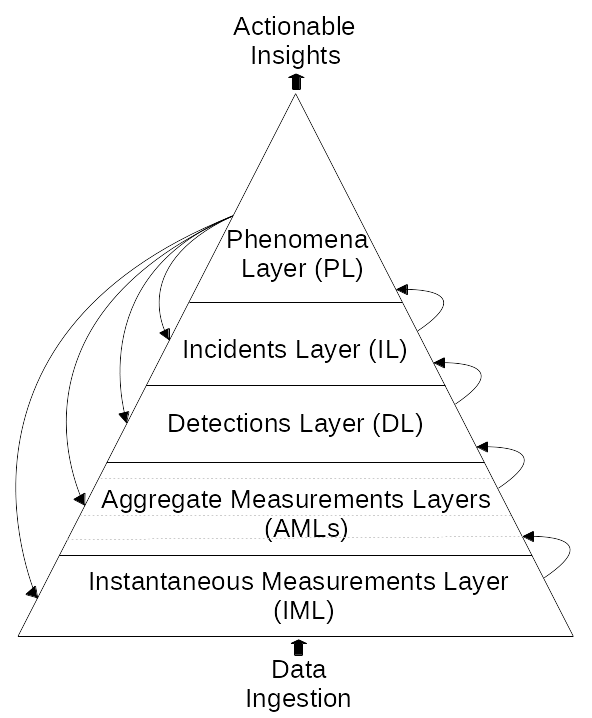
\includegraphics{figures/laha.png}	
\label{laha-figure}
\end{figure}

%\section{Five proposed benefits of Laha} \label{laha-benefits}
%Laha is designed to adaptively optimize the collection, triggering, detection, and classification of signals within a DSN. These optimizations provide several benefits to DSNs. Many of these benefits can be found in other DSNs, but generally only appear as a single optimization (TODO: CITE) or as a subset of optimizations (TODO: CITE). Laha is the first DSN to combine all of these benefits for the purpose of auto-optimizing the network.

%\subsection{Tiered management of Big Data}
%% TODO If you're going to use "Big Data" as a term of art, then it needs to be rigorously defined.
%% TODO What I think you need to emphasize here is that in any Big Data scenario, you simply can't keep all the data around forever. So, what approach will be used to decide what data to keep and what data to discard?  Laha addresses this problem by having a series of levels, each with its own TTL.  This approach has the benefit of simplifying the analysis of bandwidth and storage requirements for a DSN, but at the cost of potentially discarding important data due to the "use it or lose it" design.  Part of youer evaluation should attempt to address this weakness of use it or lose it.
%
%Laha provides tiered management of the Big Data that the framework consumes. This is mainly accomplished using the layered approach that Laha provides. All data within the Laha framework is garbage collected using a configurable time to live (TTL) for each level. As data moves from the bottom to the top of the framework, noise is discarded and only interesting data as determined by the higher levels is preserved and forwarded upwards within the framework. In this way, the network can be tuned to preserve increasingly important data. One of the drawbacks of this approach is that it's possible to accidentally discard data that does contain signals of interest, but were not detectable using the current set of detection and classification algorithms. Not only does tiered management of big data increase the signal-to-noise ratio as data is moved upwards, but it also provides graceful degradation so that data pressure is never a reason a DSN is brought down. The TTL for each level can be tuned by Laha's Phenomena to either optimize for system performance or to optimize for signal analysis The details of Laha's tiered approach can be found in section \ref{big-data-management}.
%
%\subsection{Automatically provide context to classified incidents}
%% TODO This is a feature that will be hopefully much more easily evaluated once you have the two reference implementations.  I will be interested to see what kinds of contextual information are attached, and whether there are times you wished you could attach information elsewhere.
%Laha provides Annotations Phenomena (see \ref{annotations-phenomena}) that allows users or algorithms to tag signals of interest with contextual information. There is already a large amount of research for providing classifications of signals of interest, however annotations provide context about the classifications themselves. That is, Laha provides the ability to assign causality to already classified signals.
%
%Initially, a library of annotations is required to be built for a particular DSN. Once the library has been built, Laha can provide automatic annotation assignment using similarity metrics. By using annotations and determining causality, it's possible to create actionable responses to signals observed within a network.
%
%Further, annotations can be used to optimize detection and classification of known signals. For example, imagine a power quality network that observes a voltage sag on the same sensors at the same time periodically. If the cause of the voltage sag can be determined (such as a motor turning on), then detection of this signal can either be muted or analyzed more deeply. Also, other voltage sags that exhibit similar characteristics can then be automatically annotated.
%
%\subsection{Adaptive optimizations for triggering}
%% TODO This seems totally cool, but I question whether this is a novel feature. Adaptive setting of thresholds must happen in lots of different domains.  You'll want to discuss related work here, and hopefully argue that other approaches are ad-hoc and domain-specific, but the contribution of Laha is to build adaptive optimization of triggering directly into the framework as a first-class concept. 
%Many triggering schemes rely on thresholds being surpassed within feature extracted data streams. For example, triggered data streams in a power quality network might consist of voltage, frequency, and THD extracted features to determine if there is likely a signal of interest observed from a given set of sensors. If any of the extracted features surpass a preset threshold, then we end up triggering the devices for raw, higher fidelity data. However, there are cases where the feature extracted stream may not surpass a predefined threshold and those sensors would not be triggered.
%
%By using different types of Phenomena, I can improve our triggering efficiency. For example, Locality Phenomena, as discussed in section \ref{locality-phenomena}, allow us to predict detections and classifications in space. If a particular grouping of sensors that are related in space always observe the same detections and classifications, then I can build a predictive model of when the framework can expect to see those things. In this way, a sensor may trigger on a passed threshold, but other sensors that are co-located may not trigger because feature extracted data is below the triggering threshold. If the Locality Phenomena predicts that other co-located sensors should have detected the same signal, then Laha might trigger those devices for high fidelity data to determine if the signal is in the raw data stream even though it didn't meet the triggering threshold.
%
%Laha can use Periodicity Phenomena, as discussed in section \ref{periodicity-phenomena}, in similar ways. When periodic signals are classified, Laha can create Future Phenomena that predicts when signals of interest should be detected and classified. This allows Laha to optimize triggering by tuning the triggers to specifically look for Periodic or Future Phenomena. Periodic and Future Phenomena also allows Laha to tune classification algorithms to the predicted classifications.
%
%\subsection{Adaptive optimizations for detection and classification}
%Not only can Laha optimize triggering, but similar usages of Locality and Future phenomena can be utilized to improve detection and classification efficiency. With Locality Phenomena, a model of common detections and classifications can be built for a set of co-located sensors. Detection and classification algorithms can be tuned to search for specific signals that are often observed within this model, pruning the search space and increasing the accuracy of detection and classification algorithms.
%
%Future and Periodic Phenomena provide the same benefits to detection and classification as Locality Phenomena. That is, if Laha is able to predict when a signal is going to arrive and also predict how that signal is going to be classified, then it can tune its detection and classification algorithms specifically for the signal of interest.
%
%\subsection{Provides a model of underlying sensor field topology}
%% TODO Either this is extremely cool, or totally frivolous, and I'm not sure which. it is frivolous if the only thing it's doing is detecting topology that you already know about (i.e. that two OPQ boxes are close together physically, but we already know that because of their lat/long coordinates.) it is totally cool if you are detecting topology that is not already known. So, it would be good to provide a specific example here for both domains (OPQ and Lokahi)
%
%Predictive phenomena use localization of signals to build communities or groupings of sensors that observe similar signals in both time and space. Over time, Laha can begin to build a model of the underlying topology of the sensing field. For instance, if a group of sensors always see the same signal, then we can assume that either the signal has a far reach, or the sensors are grouped together geographically. With enough sensor penetration, we can differentiate between these two scenarios.
%
%Further, if the sensors provide any sort of location information, Laha can provide a mapping from physical location to sensor field topology. This is especially useful when the topology of the sensor field is not known a priori. Even if we know the location of the sensors at all times, that does not mean that we understand the topology of the sensing field. For example, in a PQ network, the topology is defined by how the electrical grid is connected to itself and laid out. Laha hopes to provide a model that can determine the electrical distance between devices even if the topology of the grid is not known. As another example, take an infrasound network. It's possible that two sensors are located close to each other geographically, but if they have a large mass between them, they may not receive the same signals due to the topology of the environment around them. 
%
%In this sense, Laha is not interested in knowing the location of sensors relative to each other, but is more interested in understanding how signals flow between sensors as a constraint on the topology that the signals travel through. That is, can Laha determine the statistical signal distance between sensors? And if it can, can the model be used to further tune lower levels of the Laha hierarchy?
%
%The aim is that if Laha can accurately provide a model of the underlying sensing field topology, this information can be used to optimize lower levels of the Laha hierarchy. For example, Laha can prime sensors for receiving or ignoring signals of interest by determining that a signal is supposed to arrive at a sensor before it does, i.e. Predictive Phenomena.

\section{Big Data Management in Laha} \label{big-data-management}
The Laha framework acts as an adaptive sieve for filtering noise and uninteresting data collected from a DSN. In this way, each level only passes what it considers interesting to the level above it. All data at a particular level is garbage collected at specific intervals relating to its important to the DSN.

Each level only keeps data for a specified amount of time before it is garbage collected. As data moves up the pyramid, it is generally considered more useful and therefore has a longer Time to Live (TTL), the amount of the time the data lives before it is garbage collected.  When a higher level detects ``something interesting", the data contained in the time window of ``something interesting" is copied into the levels above it and will still persist even though the original data is garbage collected. In this way, Laha preserves data from all levels if they are associated with interesting data. This also provides graceful degradation of services. The TTL is managed by the overall memory management of the system. Laha Actors are designed to work within the constraints of the TTL at different levels. If a constraint is broken, the Actor logs this issue. TTL can be optimized by Phenomena at each level to either tune for system performance or tune for decreasing of false positives and false negatives at different levels within the Laha hierarchy.

A summary of how data management in Laha is provided in table \ref{data-managament-table}. Note that the TTL is configurable for each implementing network and the table provides default values.

\begin{table}
	\caption{Summary of data management and context addition in Laha}
	\begin{tabular}{|c|c|c|}
		\hline 
		Level & Description & Time-to-Live (TTL) \\ 
		\hline 
		Phenomena Level (PL) & Contextual \& predictive analytics &  \\ 
		\hline 
		Incidents Level (IL) & Classified signals &  1 year \\ 
		\hline 
		Detections Level (DL) & Triggered windowed raw data & 1 week  \\ 
		\hline 
		Aggregate Measurements Level (AML) & Statistical aggregates of raw data  & 1 day  \\ 
		\hline 
		Instantaneous Measurements Level (IML) & Raw sensor data  & 1 hour \\ 
		\hline 
	\end{tabular} 
    \label{data-managament-table}
\end{table}

\subsection{Instantaneous Measurements Level}
The Instantaneous Measurements Level (IML) receives raw, sampled data from the DSN. The amount of data received is determined by the sample rate of each device multiplied by the number of fields per sample. Most of the time samples, from devices in the network are mainly sampling noise. A large percentage of the data in this level is destined for garbage collection and data is assigned a Time to Live (TTL) of one hour. 

\subsection{Aggregate Measurements Level}
The Aggregate Measurements Level (AML) is responsible for rolling up IMs from the IML. In general, this level only works with feature extracted data, rather than working with the raw samples. Each measurement in the AML provides summary statistics over a configurable time window. For example, these can include min, max, mean, median, mode, and variance statistics. 

It's possible to breakup the AML into several sub levels, each with different window sizes. For example, Laha might roll IMs into one minute AMs, then roll one minute AMs into hour AMs, then days, and so on. Each sublevel within the AML can have its own configurable TTL, ensuring long term summary statistics stick around for as long as needed. This provides us a high level view of the network and can provide insights into long term trends which wouldn't be visible (or available) in the IM data stream.

Similar to IMs, AMs can be saved and copied to the levels above it when interesting data is observed. This ability allows for AMs during these time periods to be stored and saved from the garbage collection process.

At this point in the hierarchy, we are still not providing any context to the data that we are receiving. Context is provided by levels above the AML.

\subsection{Detections Level}
The Detections Level (DL) is the first level that provides some context to the data that the sink is receiving. This level is responsible watching the feature extracted data streams, and requesting IMs from the IM level. In general, the detection level is meant to be trigger happy\footnote{Pun intended.} and be overly aggressive when determining if a feature extracted data stream looks interesting. 

When a data stream looks interesting, the DL marks a timestamp $N$ seconds before the interesting features and $M$ seconds after the interesting features, where both $N$ and $M$ are configurable within the framework. The goal is to use a time window that catches signals of interest within it. Since these data ranges will be further processed and refined higher in the hierarchy, there is no issue with collecting larges amounts of data in this level. 

The actual methods of detection is dependent on the characteristics of every individual sensor network. This framework assumes that the detection algorithms are provided by the implementing frameworks.

Similar to other levels, the DL level will have its IMs and AMs copied into levels above it when upper levels observe something interesting in the DL. The detections level is set to have a TTL of a week.

\subsection{Incidents Level}
Incidents represent classified signals. Incidents are individual classifications for signals of interest and are created by analyzing waveforms from Events. Waveforms from Events may contain multiple incidents. Individual signals may be classified as multiple incidents (for example a transient being classified as both a transient and frequency incidents). 

Incidents are further analyzed to produce phenomena. 

Incidents are expired after one year of storage. 


\subsection{Phenomena Level}
Phenomena are defined as a grouping of incidents that provide one or more of annotations, locality, periodicity, predictiveness, similarity, and future phenomena. 

Not only do Phenomena provide interesting insight and analytics into the underlying data, but they also provide a means for adaptively tuning the underlying collection, triggering, detection, and analysis of a distributed sensor network.

Phenomena are summarized in table \ref{phenomena-summary-table} and discussed in great detail in section \ref{phenomena}.

\section{Phenomena: Providing Adaptive Optimizations in Laha} \label{phenomena}

\begin{table}
	\centering
	\caption{Summary of Laha Phenomena}
	\begin{tabular}{|c|c|}
		\hline
		Phenomena & Description \\
		\hline
		Annotations & Provide context about an Incident or set of incidents \\
		\hline
		Locality & Provides context on how incidents are related in time and space \\
		\hline
		Periodicity & Designation for incidents that exhibit repetitive or periodic behavior \\ 
		\hline
		Similarity & Subset of incidents found using grouping and community detection algorithms \\
		\hline
		Predictive & Subset of incidents characterized by predictive or forecasting models\\
		\hline
		Future & Incidents scheduled to occur in the future\\
		\hline
	\end{tabular}
	\label{phenomena-summary-table}
\end{table}

\subsection{Annotations Phenomena} \label{annotations-phenomena}
Annotations provide context about an Incident or a set of Incidents. Annotations are generally user provided or sourced from other data sources to provide supporting context to Incidents. For example, Annotations might include “Cloud Cover”, “Hurricane Hector”, “Dryer Turns On”, etc.

In some sense, annotations allow us to label our data sets beyond a simple classification and start looking at causal classifications. Once enough annotations have been assigned to classified incidents, Laha can used Annotations to attempt to label unknown incidents with similar characteristics.

Annotations can be used to tune Laha's detection and classification algorithms by allowing Laha to filter on incidents with known causes.

\subsection{Locality Phenomena} \label{locality-phenomena}
Locality provides context on how incidents are related to each other in both space in time. Laha is able to determine if classified incidents are local to a single sensor, to a group of co-located sensors, or global across an entire network. Sensors can be co-located in both the physical sense and also co-located within a sensing field. For example, sensors in a power quality network may be separated by large distance geographically, but co-located through the electrical grid and the grid's topology. 

Over time, Locality Phenomena is used to build a model of sensors in relation to each other and to provide a statistical likelihood that co-located sensors will observe the same signal. Locality phenomena can be used to drive network triggering, detection, and classification thresholds within a distributed sensor network by using this probabilistic model for determining the likelihood that a sensor or sensors will observe a signal of interest.

\subsection{Periodicity Phenomena} \label{periodicity-phenomena}
Periodic phenomena consists of incidents that exhibit repetitive behavior, that is, the same types of incidents appearing in cycles from single or multiple devices. Periodicity allows for the easy creation of Predictive phenomena.

Periodic phenomena can come from a single incident or from multiple incidents. Periodic phenomena allow us to either tune our network to find periodic incidents or tune the  network to ignore periodic incidents depending on if the incidents are of interest. Periodic phenomena are especially useful in conjunction with Annotation phenomena as Laha can assign causality to the periodic signal. 

\subsection{Similarity Phenomena}
Similarity phenomena utilize grouping and community detection algorithms to group incidents together by their features. Common features used for grouping include time, location, incident type, or incident features.

\subsection{Predictive Phenomena}
Predictive phenomena consists of incidents that are characterized by a predictive or forecasting models. Predictiveness is a behavior that can be inferred from all other phenomena types. 

Predictiveness is the main driver behind optimizing the control of a distributed sensor network. If Laha can predict the types of signals that will arrive at sensors, then Laha can tune those sensors and the sink to either filter the signals (if the user is not interested in signals) or tune the sensors and the sink to be extra sensitive to those signals, possible detecting them even if they previously would not have been detected.

\subsection{Future Phenomena}
Predictive phenomena can be used to create future phenomena. Future phenomena are a statistical model of the likelihood of seeing an incident or incidents at future points in time. Knowing that a signal may occur with some probability allows Actor affected by those signals time to prepare for the signals.

\section{Laha Actors: Acting on the Laha Data Model}
Laha Actors act on the Laha hierarchy and provide one of two functions. Actors can move data from one level of the hierarchy upwards through the hierarchy when interesting data is requested by an upper level. Actors can also apply adaptive optimizations downwards through the hierarchy. The Laha framework can support multiple actors at each level. For example, the Incidents Level in our reference power quality network contains actors for each of the following functions: IEEE classified voltage events, frequency variations, power outages, excessive THD, and many others. The Incident Level Actors move data from these incidents upwards to the Phenomena Level.  

Table \ref{laha-actors-tables} summarizes the actors that exist within the Laha framework and their purposes. 

\begin{table}
	\centering
	\caption{Summary of Laha Actors}
	\begin{tabular}{|c|c|}
		\hline
		Actor & Purpose \\
		\hline
		IML Actors & Perform feature extraction and move aggregate data to AML \\
		\hline
		AML Actors & Perform triggering on data from IML, copy data to DL if interesting \\
		\hline
		DL Actors & Perform high fidelity feature extraction on possible detections \\
		\hline
		IL Actors & Perform classification and contextualization on possible detections \\
		\hline
		PL Actors & Generate predictive analytics and optimize the lower levels of the hierarchy \\
		\hline
	\end{tabular}
	\label{laha-actors-tables}
\end{table}

\subsection{Actor Constraints}
Actors at each level in the hierarchy are governed by a set of constraints. These constraints include the set of possible inputs, $A_i$, the set of possible outputs, $A_o$, the set of Actors it can receive data from, $A_{ai}$, the set of Actors it can transmit data to, $A_{ao}$, and a set of performance metrics that each actor must maintain, $A_p$. The constraints assigned to each Actor are determined by the hierarchy level in which the Actor resides.  

Actors are responsible for reporting constraint violations and in this way, Actors are the primary provider of health, performance, and status metrics about the Laha framework.

The constraints for each level of Laha hierarchy is summarized in table \ref{actor-constraint-table}.

\begin{table}
	\centering
	\caption{Summary of Laha Actor Constraints at Each Level}
	\begin{tabular}{|c|c|c|c|c|c|}
		\hline
		Level & $A_i$ & $Ao$ & $A_{ai}$ & $A_{ao}$ & $A_p$ \\
		\hline
		IML & Raw samples & Aggregate trends & n/a & AML & Data ranges available \\
		\hline
		AML & Aggregate trends & Detections & IML & DL & Data ranges available \\
		\hline
		DL & Windowed waveforms & Hi-fi extracted features & AML & IL & Data \& features available \\
		\hline
		IL & Hi-fi extracted features & Contextualized incidents & DL & PL & Incident types available \\
		\hline
		PL & Contextualized incidents & Optimizations & IL & All levels & Optimizations available \\
		\hline
	\end{tabular}
	\label{actor-constraint-table}
\end{table}

\section{OPQ: A Laha-compliant Power Quality DSN}
OPQMauka is a middleware component of the Open Power Quality (OPQ) framework. The OPQ project provides a hardware and software solution for monitoring distributed power quality (PQ). The OPQ project was founded with the goal of studying how intermittent distributed renewable energy sources affect PQ not just at a user's home, but also within a user's neighborhood, between neighborhoods, and globally across the grid. 

The OPQ ecosystem is made up of networked hardware sensors (OPQBoxes) and various software services (OPQMakai, OPQMauka OPQHealth, OPQView). Each of these software components are made up of individual services and plugins.

The OPQ system design is laid out in figure \ref{fig:opq-system}.

\begin{figure}
	\centering
	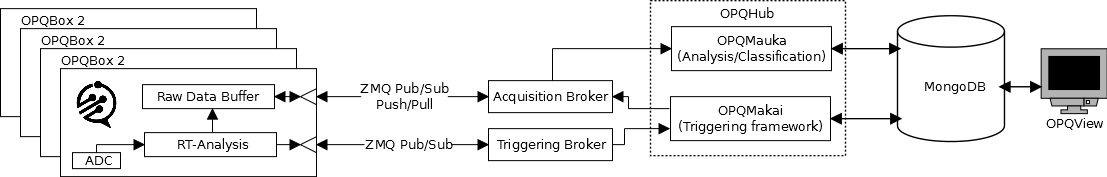
\includegraphics[width=\linewidth]{figures/system-diagram.png}
	\caption{OPQ System Diagram}\label{fig:opq-system}
\end{figure}
%
%\subsection{OPQ: Boxes}
%An OPQ Box is a custom designed PQ sensor. OPQBoxes can be plugged into a wall outlet and communicate with OPQ servers using the user's WiFi connection. OPQBoxes consist of a Raspberry PI single board computer (SBC), a custom board for PQ measurements, custom firmware, and a custom enclosure. The custom board contains an ADC that samples an alternating current (AC) power signal at 12 thousand samples per second. This data is transferred to the Raspberry Pi where feature extraction and data transfer takes place. The hardware design is presented in figure \ref{fig:opq-box-design} and the software design is provided in figure \ref{}.
%
%\begin{figure}
%	\centering
%	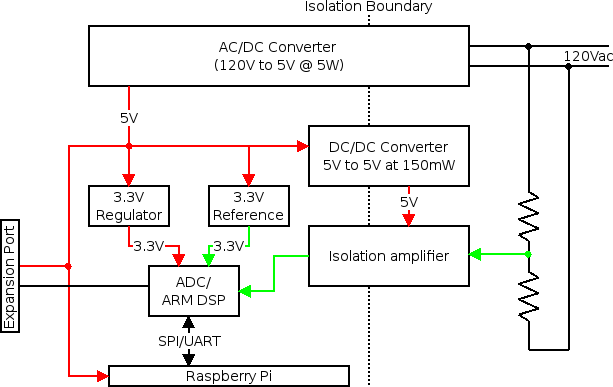
\includegraphics[width=.75\linewidth]{figures/opqbox_diagram.png}
%	\caption{OPQ Box Design}\label{fig:opq-box-design}
%\end{figure}
%
%\begin{figure}
%	\centering
%	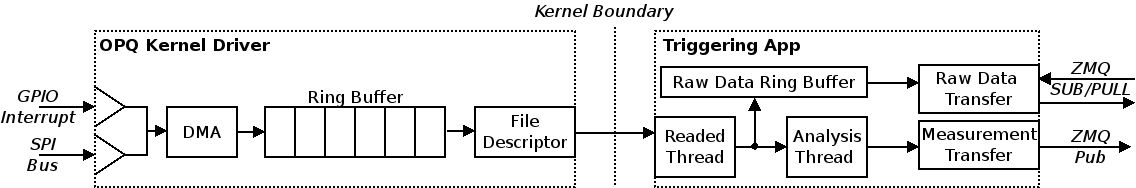
\includegraphics[width=.75\linewidth]{figures/opqbox_software.png}
%	\caption{OPQ Box Software}\label{fig:opq-box-software}
%\end{figure}
%
%The feature extraction algorithms extract from the sampled waveform the following features: windowed $V_{RMS}$, frequency, and total harmonic distortion (THD) features. The feature extracted data is then sent to a central sink where further analysis is used to determine if the sensor or a subset of sensors should be triggered for raw data.
%
%The OPQ network is a hybrid network that uses edge computing for calculating features at the edge of the network. This is opposed to networks that utilize a ``send everything" approach. In this way, Laha is able to minimize bandwidth. 
%
%OPQBoxes are synchronized to each other and the OPQ back end using the network time protocol (NTP). This provides synchronization to the millisecond level, which although is great for longer incidents, does not provide accurate timing for transients that may be shorter than tens of milliseconds.
%
%
%\subsection{OPQ: Makai}
%OPQ Makai is the central sink and triggering daemon for the OPQ framework. It is made up of several services which are responsible for aggregating and processing the measurements generated by OPQ Boxes. Low fidelity feature extracted data consisting of $V_{RMS}$, frequency, and THD are streamed from OPQ Boxes at a configurable message rate. These data streams are observed by OPQ Makai and the daemon uses statistical methods and thresholds to determine if the sensor or a subset of sensors should be triggered for a window of raw sampled waveforms. 
%
%The OPQMakai system design is provided in figure \ref{fig:makai-main}.
%
%\begin{figure}
%	\centering
%	\includegraphics[width=.75\linewidth]{figures/makai_main.pdf}
%	\caption{OPQ Makai Design}\label{fig:makai-main}
%\end{figure}
%
%\subsection{OPQ: Health}
%OPQHealth is a service that continuously monitors both the hardware sensors and the software services that make up the OPQ framework.
%
%OPQHealth detects health issues in the following ways. 
%
%OPQHealth determines if an OPQBox is active or inactive by querying the Mongo database for the most recent aggregate measurement. If there is a record of an aggregate measurement within 5 minutes, the Box is considered up, otherwise it is considered down.
%
%The status of OPQMakai is determined by Makai inserting special health events into the Mongo database. Health queries for the presence of these events and if events are not observed within 1 minute, the OPQMakai service is considered down.
%
%OPQMauka provides a special HTTP endpoint that is only accessible within the OPQ back end network that when accessed with a \textit{GET} request will return with a status of \textit{200 OK} if the service is up and available. Any other response of the absence of the response is considered a failure more for OPQMauka.
%
%MongoDB is monitored by querying for a sentinel value that was previously placed in the database.
%
%OPQView is monitored by sending a \textit{GET} request to the landing page. A response of \textit{200 OK} means that the health service is up. Any other response or the lack of response is an indication of failure for OPQView.
%
%OPQHealth stores its findings in both the Mongo database as well as in a traditional log file.
%
%\subsection{OPQ: View}
%OPQView is a web application that provides visualization, notification, and user management services for data, sensors, and user accounts with the OPQ framework. OPQView is built using Meteor.js and provides a Reactive view of the underlying data stored in the OPQ database.
%
%A screenshot of OPQView in action is provided in figure \ref{fig:opq-view}.
%
%\begin{figure}
%	\centering
%	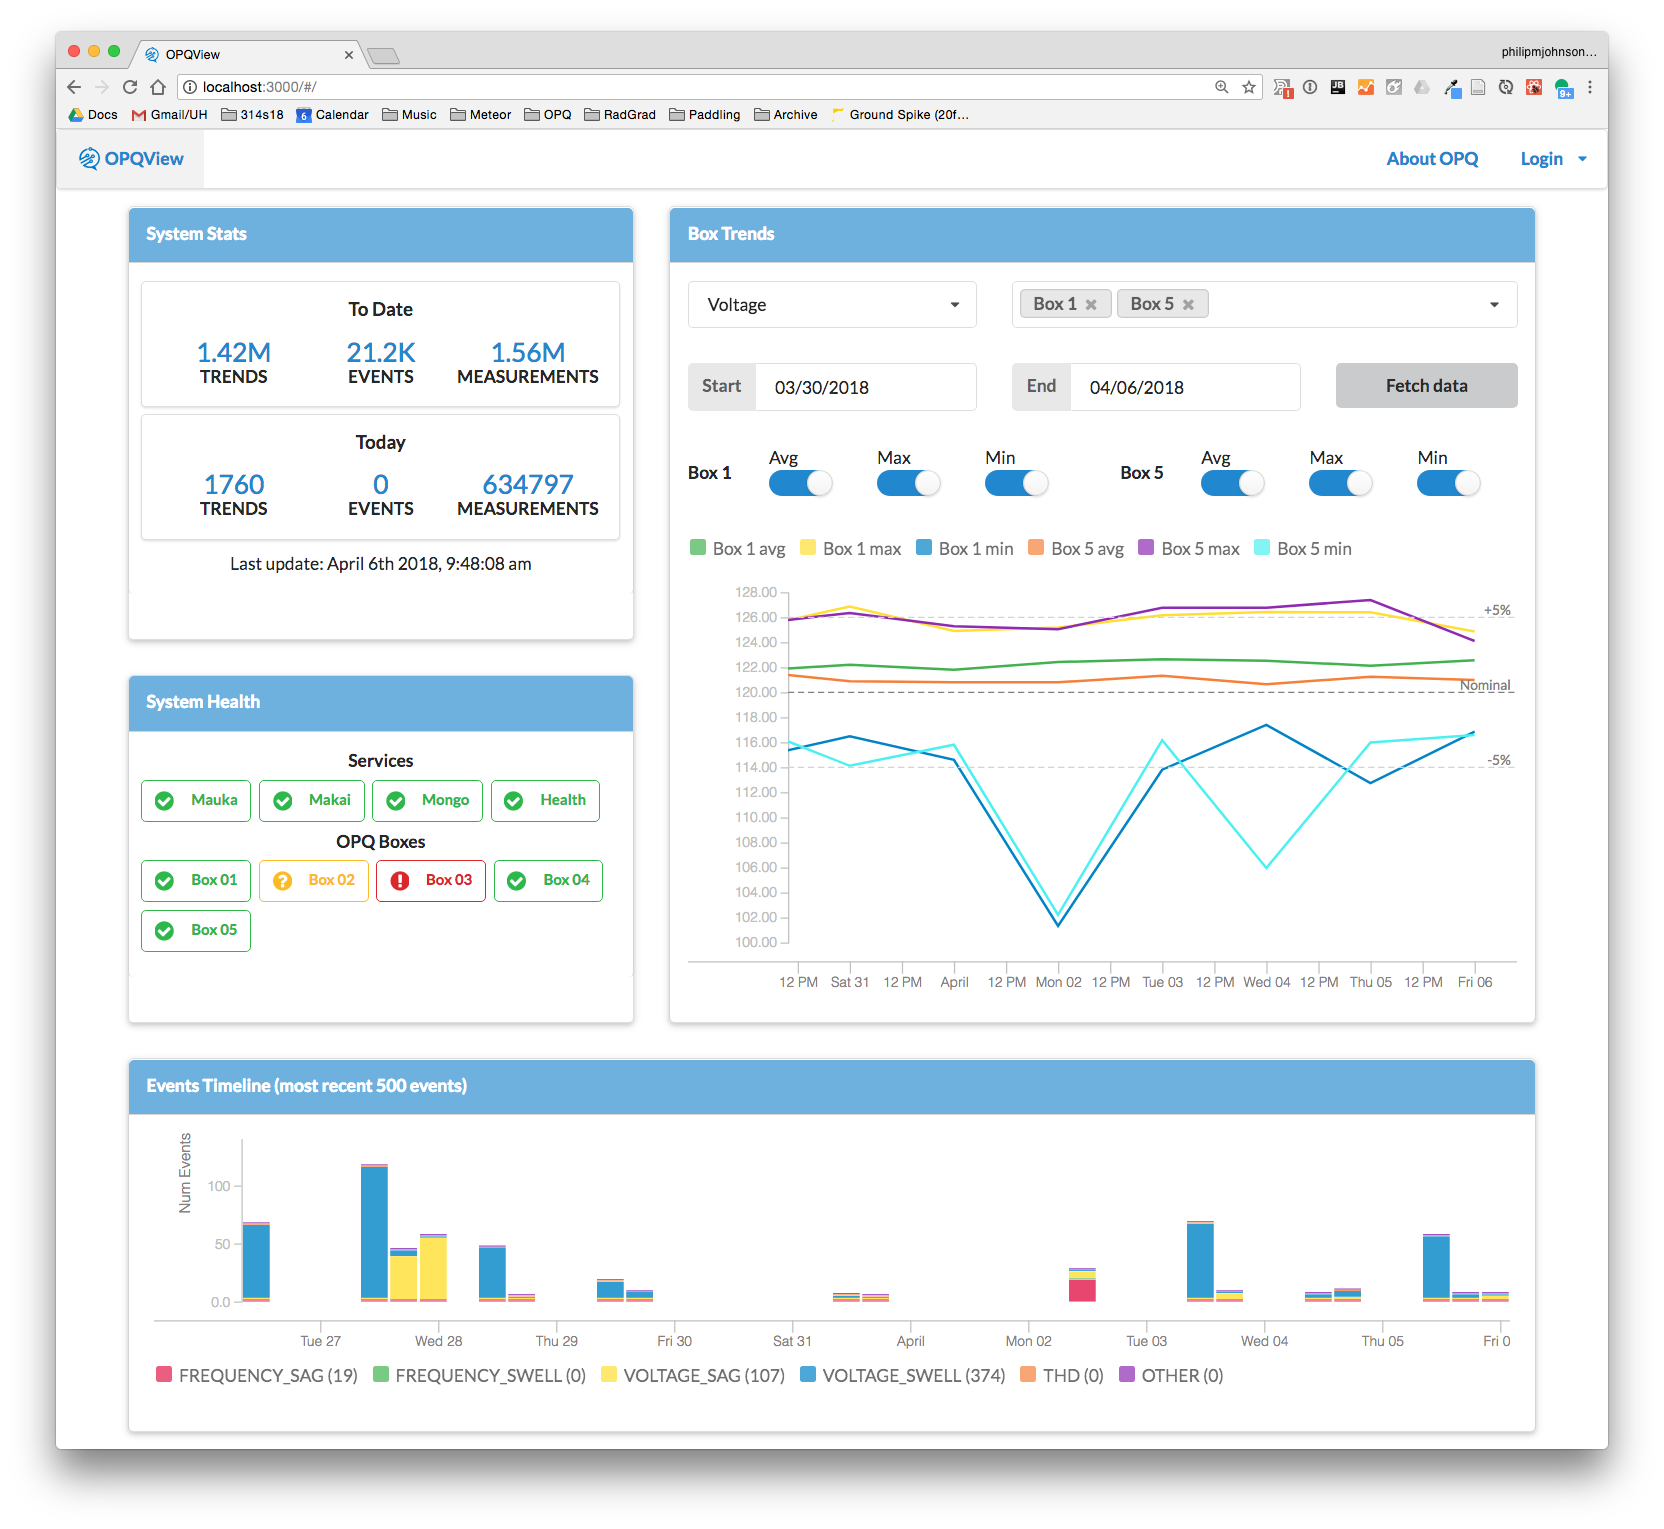
\includegraphics[width=1\linewidth]{figures/opqview-landing-page.png}
%	\caption{OPQ View Screenshot}\label{fig:opq-view}
%\end{figure}
%
%\subsection{OPQ: Mauka}
%% TODO
%
%TODO: This section is in the making and will be much more detailed than the other components of OPQ.
%
%\subsection{OPQ: Data Model}
%% TODO

%\subsection{OPQ as a Laha-compliant DSN}
%OPQ and specifically OPQMauka comply with the Laha abstract framework. Table \ref{opq-compliance} summarizes how the OPQ data architecture fits within the Laha conceptual model.
%
%\begin{table}
%	\caption{OPQ as a Laha-compliant DSN}
%	\begin{tabular}{|c|c|c|c|c|}
%		\hline 
%		Laha Level & OPQ & Created By & Stored By & TTL \\ 
%		\hline 
%		IML & raw ADC Samples & OPQBox & Onboard memory & 20 minutes \\ 
%		\hline 
%		AML & min,max,avg V, F, THD & OPQBox & trends\footnotemark & 1 day \\ 
%		\hline 	
%		DL & triggered waveforms & Makai/Mauka & events/box\_events\textsuperscript{\ref{fn-1}} & 1 week \\
%		\hline
%		IL & Classified detections & Mauka & incidents\textsuperscript{\ref{fn-1}} & 1 year \\
%		\hline
%		PL & Predictive analytics & Mauka & phenomena\textsuperscript{\ref{fn-1}} & N/A \\
%		\hline
%	\end{tabular}
%	\label{opq-compliance}
%\end{table}  
%\footnotetext{MongoDB Collection Name\label{fn-1}}
%
%In order to be a Laha compliant DSN, the reference DSN must also implement Laha Actors. Table \ref{opq-actors} summarizes how OPQ implements Laha actors.
%
%\begin{table}
%	\caption{OPQ  Actors Implementation}
%	\begin{tabular}{|c|c|c|}
%		\hline 
%		Laha Actors & OPQ Equivalent & Description \\ 
%		\hline
%		IML Actors & Boxes & Store window of raw sensor samples \\
%		\hline
%		AML Actors & Boxes \& Makai & Makai stores and triggers on aggregate data from Boxes \\
%		\hline
%		DL Actors & Mauka & MakaiEvent plugin \\
%		\hline
%		IL Actors & Mauka & Voltage, Frequency, THD, Outage, plugins \\
%		\hline
%		PL Actors & Mauka & Annotations, Locality, Similarity,  Periodic, Predictive,  Future plugins\\
%		\hline
%	\end{tabular}
%	\label{opq-actors}
%\end{table}  

\section{Lokahi: A Laha-compliant Infrasound DSN}
Lokahi is a dynamic DSN that originally evolved as a distributed infrasound detection network. Infrasound is characterized as sound waves that are less than 20 Hz. Infrasound generally can not be deciphered by the human ear, but it can be detected using microphone and barometric pressure sensors. Any large movements of the atmosphere can produce infrasound. The Lokahi network was designed to supplement the International Monitoring System (IMS) for the capture  of undeclared and declared nuclear explosions. Lokahi has been successfully used to capture signals from volcanoes, hurricanes, aircraft, meteors, and other large atmospheric events. 

Sensors in Lokahi are any mobile device that can run iOS or Android. We have sensors distributed world wide. The software stack for Lokahi consists of a distributed actor system for data acquisition, MongoDB for metadata persistence, Apache Kafka for data queues and interprocess communication, Python and related scientific libraries for analysis, and a distributed key-value store for long term storage or sensor data.

Recent development and improvements to the data API have allowed Lokahi to begin accepting data from any of the available onboard sensors on iOS and Android devices. Even though the main focus is still infrasound, having access to all of the available sensors provides the ability to sense other sensor fields and to perform interesting data fusion techniques. 

A diagram of the Lokahi framework is provided in figure \ref{fig:lokahi}.


\begin{figure}
	\centering
	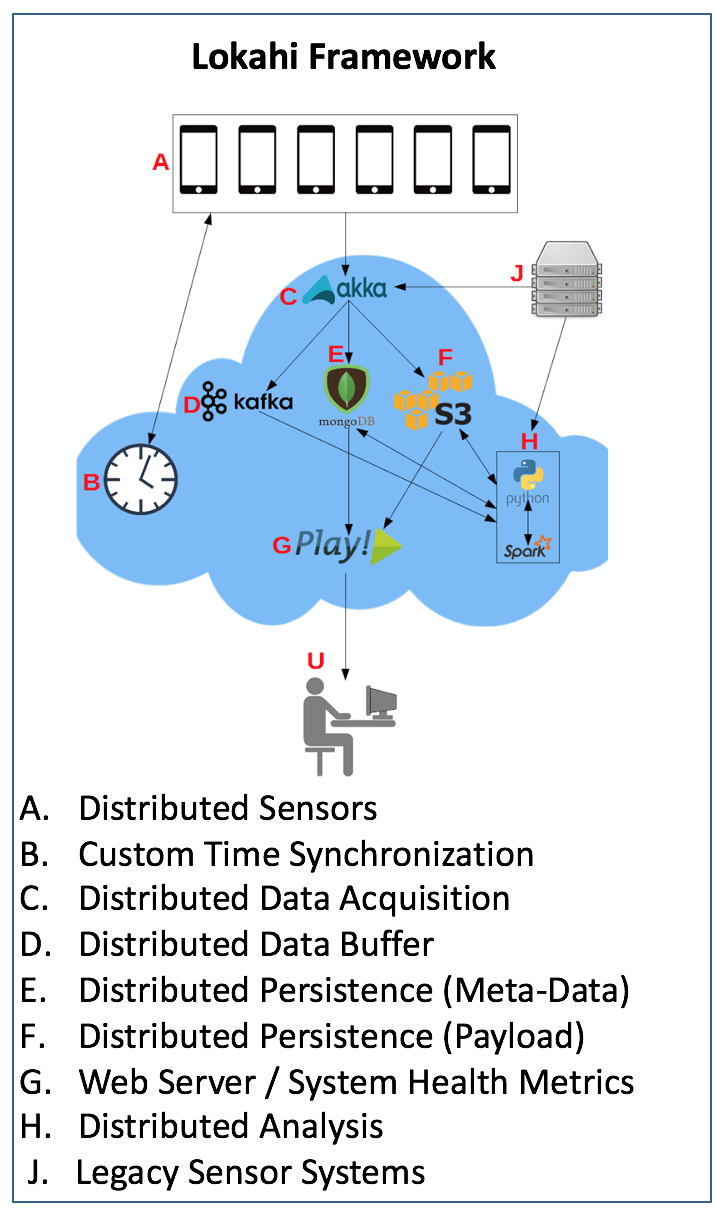
\includegraphics[]{figures/lokahi.png}
	\caption{Lokahi Design}\label{fig:lokahi}
\end{figure}

%\subsubsection{Lokahi: Ingestion}
%Unlike OPQ, Lokahi takes an approach of send and store everything from every sensor, all the time. This approach is vastly different than what we're used to in triggering based acquisition systems. Data between sensors and our Ingestion servers is encrypted using standard SSL encryption algorithms. Authentication and authorization for each sensor is accomplished using Json Web Tokens (JWTs) with signatures generated using elliptic curve cryptography (ECC). Data at the sensor level is serialized using protocol buffers and then compressed using LZ4. 
%
%To enable the smooth retrieval of large amounts of sensor data, Lokahi uses a distributed actor system (Akka) to automatically scale horizontally based on the current volume of data being received. 
%
%\subsubsection{Lokahi: Persistence}
%Metadata is stripped from the sensor data at data ingestion and immediate stored to a distributed Mongo database. Metadata is indexed using a combination of device id and timestamps. 
%
%Metadata drives the rest of the Lokahi framework and provides pointers to the raw data.
%
%Raw sensor data is stored in a distributed key-value store. Lokahi uses Amazon's Simple Storage Service (S3) which provides automatic data redundancy and essentially limitless storage. Raw sensor data is stored by key and the key is stored in the metadata.
%
%Raw sensor data is also persisted in an Apache Kafka queue. Kafka not only provides the framework with a message queue to pass data between distributed services, but it also acts as a ring buffer. Each sensor stores 1 hours worth of data in Kafka that can be looked up by any of the distributed clients and retrieved very quickly. For those reasons, Kafka powers IPC and data buffering roles for our real time analysis of Lokahi sensor data streams.  
%
%\subsubsection{Lokahi: Analysis}
%Analysis in Lokahi is provided by a set of distributed processes that were developed in Python using SciPy, NumPy, and matplotlib. Recent developments in the framework are now also including the basis for machine learning (ML) using Tensor Flow.
%
%We provide real time plotting and analysis by subscribing to real time data feeds provided by the Apache Kafka real time queue and buffer. We also provide more robust batch analysis of historical data that can be initiated from Lokahi Web.
%
%
%\subsubsection{Lokahi: Web}
%Lokahi web is a web application for querying and performing analysis of real time sensor data or over historical sensor data. Lokahi also has built in system of health displays for providing a real-time and historic overview of the health of the distributed services within the framework. 
%
%% TODO, provide screenshot

%\subsubsection{Lokahi as a Laha-compliant DSN}
%TODO
\chapter{Evaluation}
Evaluation of the Laha framework involves deploying reference Laha-compliant DSNs, validating the data collected from the reference implementations, and then comparing and contrasting various metrics for each of the stated goals. Metrics were collected during a set of experiments for each of the Laha reference implementations in early 2019. 

The following sections describe my plans for deployment of reference implementations, data validation, evaluating the main goals of the Laha framework, and evaluating the tertiary goals of the Laha framework.

\section{Deploy Laha reference implementations on test sites}
In Q2 and Q3 2019, 15 Laha-compliant OPQBoxes were deployed on the University of Hawaii at Manoa's power microgrid. Using a provided blueprint of the microgrid as a guide and collaborating with the Office of Energy Management, these sensors were placed strategically with the hopes of observing PQ signals on the same line, PQ signals generated from intermittent renewables, local PQ signals, global PQ signals, and PQ signals near sensitive lab electronics. Many of these sensors are co-located with industry standard PQ monitoring systems. The industry standard sensors provide both ground truth and a means of comparison between a Laha designed network and a non-Laha designed network.. 

In Q3 2019,  20 to 30 Laha-compliant Lokahi sensors were deployed near and around the Infrasound Laboratory in Kailua-Kona on the Big Island of Hawaii. These sensors were be placed strategically around a calibrated infrasound source. The sensors were placed with the assistance of Dr. Milton Garces to ensure that I can target sensors at different distances by tuning the amplitude and frequencies of the infrasound signal. In this way, I know which devices should or should not have received the signal.

\section{Validate data collected by Laha deployment}
Beginning in Q1 2019, I  began validated data collection from both the OPQ network and the Lokahi network. 

Data was validated in the OPQ network be comparing detected and classified signals against industry standard meters that are co-located with our sensors. Data validation is an autonomous process that validates signals and trends seen in both the industry sensor and the OPQ sensors. Data validation provides metrics for signals and trends that the reference sensors observed but OPQ sensors did not (false negatives) as well as signals that the OPQ sensors observed and the reference sensors did not (false negatives).  Specifically, I looked to compare long term trends (voltage, frequency, and THD readings over a time period of days) as well as more transient signals of interest (i.e. voltage sags/swells, frequency variations, excessive THD, and outages).

Data from the Lokahi network was validated against industry standard infrasound sensors. We also control the amplitude and frequency of the signals generated from the calibrated infrasound source and can use geophysical equations to predict which sensors should have seen or not seen an infrasonic signal. Data validation is autonomous for this network as well. Similar to the OPQ network, I collected metrics on false positive and false negatives as compared to the reference sensors. 

Data validation for both networks continued for all data collection until the end of the project.

\section{Use Laha deployments to evaluate the main goals of the framework}
The Laha deployments for both OPQ and Lokahi were used to evaluate each of the main goals this framework claims to provide. Namely that Laha is a generally useful framework representation for DSNs. Second, Laha provides the ability to turn primitive sensor data into actionable data and insights. Third, Laha's tiered management of sensor data provides metrics on maximum bounds for storage requirements and graceful degradation of DSN performance. 

Each deployment requires different techniques for performing evaluation. 

In the OPQ deployment, OPQBoxes are deployed and co-located with industry standard, calibrated, reference sensors. Each of these sensors cost thousands to obtain and install, collect all the data all the time, and can only be connected to the power main as it enters a building. These sensors provide a means for verifying signals received or not received by OPQ, as well as confirming long term trend data. I have been provided access to these sensors and stored data via the Office of Energy Management at UH Manoa. The data is accessible via an HTTP API. The Office of Energy Management at UH Manoa has also provided the full schematics for the UH power grid. This was used as a ground truth for topology estimates and distributed signal analysis. OPQBoxes are placed in strategic locations on the UH Manoa campus specifically in order to evaluate the distributed nature of PQ signals. For example, OPQBoxes are placed on the same electrical lines as well as separate electrical lines to observe how PQ signals travel through an electrical grid.

In the Lokahi deployment, I had the opportunity to generate infrasound signals using a calibrated infrasound source \cite{park2009rotary}.. The source can be tuned to produce infrasound at configurable frequencies and amplitudes. The source works by attaching a variable pitch propeller to an electric motor that can be driven by a waveform generator. The source can generate signals that can be observed at large stand off distances, over tens of kilometers. Similar to the OPQ deployment, sensors within the Lokahi deployment were co-located with industry standard, calibrated, infrasound sensors. These sensors can provide a metric of signals that were correctly observed, incorrectly observed, or not observed at all by the Lokahi deployment. Further, infrasound itself is characterized quite well by various geophysical equations. These equations can be used to predict if sensors deployed in the Lokahi deployment are likely to observe generated infrasound signals.

Evaluation of the main goals of this network are provided in the following sections.

\subsection{Evaluation of the Generality of this Framework}
I claim that the Laha framework is useful and general enough to be applied to DSNs in different domains. To test this, I designed, developed, and deployed two DSNs. The first OPQ, measures distributed PQ signals on the electrical grid. The second, Lokahi, observes infrasound signals traveling through the atmosphere. 

To evaluate the generality of the Laha design, I provided metrics for whether or not each deployment is able to fulfill the goals of the given network.

I expect the PQ network, OPQ, to be able to detect and classify common PQ issues. I expect OPQ to observe voltage dips, voltages swells, frequency dips, frequency swells, transients, and high levels of THD. A count of these signals were kept and compared against industry standard PQ meters co-located with each sensor. By comparing these signals to the ground truth, we were able to tabulate a number of false positives and false negatives. In order to be considered effective, I would expect to be able to classify each of these common PQ signals, collect a set of each of the PQ signals while maintaining a low number of false positives and false negatives as compared to the industry standard sensors. In general, a negative result here would be not being able to detect PQ signals of a specific type or having a high number of false positives or false negatives.

Further, another stated goal of OPQ is to detect and classify distributed PQ incidents. That is, PQ signals that are observed by more than one sensor in situations where OPQ sensors are not co-located. First, I evaluateed if OPQ is capable of detecting distributed PQ signals. I expect OPQ to at least observe one distributed signal during the test deployment, but would not be surprised to see many. By working with the Office for Energy Management at UH Manoa, I used a list of known PQ source events along with signals collected by OPQ and the industry standard sensors to provide a list of false positives and false negatives for the number of distributed PQ incidents observed by OPQ.

I expect the infrasound network, Lokahi, to be able to securely detect and report on infrasound incidents from a large collection of heterogeneous smartphone based infrasound sensors. This network prioritizes availability and security even in the face of network issues or no network at all. I claim that Laha is a useful framework for a DSN such as this and evaluated if Laha is able to meet the goals of this network.

To evaluate the effectiveness of Laha as implemented by Lokahi, I deployed 50 heterogeneous Lokahi smartphone sensors at predetermined distances from a calibrated infrasound source. I then used the calibrated infrasound source to generate infrasound signals of different amplitudes and frequencies. While signals are being generated, I disabled network access for the sensors to simulate real life network drop outs of sensors. I disabled the networks for time periods of 1 minute, 30 minutes, and 1 hour. 

Then, for each sensor, I calculated the number of false positives and false negatives for detections of infrasound signals. In order for Laha to be a useful framework for Lokahi, Lokahi must demonstrate that not only can it detect infrasound signals at different frequencies and amplitudes, but it must also do this while maintaining a low number of false positives or false negatives. 

Further, as availability is a major priority of this network, network outages must be handled without signal loss. To evaluate this goal, I measureed the amount of false negatives (or missed signals) due to Laha's data management and the interplay with network outages. I would expect that if Lokahi implements it correctly, we should not see a rise in false negatives. A less great result would be an increase in false negatives.

Finally, backed by the metrics for both deployments, I provide a critical discussion on what types of DSNs Laha is well suited for and what types of DSNs Laha is not well suited for. This includes a discussion on which parts of the Laha design are useful or a detriment to a given goal of the DSN.

The following sections continue to discuss the evaluation strategies required to show that Laha is a generally useful representation for a DSN.

\subsection{Evaluation of Converting Primitive Data into Actionable Insights}
An important goal of any DSN is to convert primitive sensor data into actionable insights. This is generally accomplished by adding some kind of context associated with the data such as classifications of a signal or linking the data with other data by comparing similarities in time, space, or other physical features.

I claim that Laha's use of Actors acting on and moving data between levels in the Laha hierarchy provides a useful and generic approach to systematically adding context to data as it moves through the framework. Laha is designed with a specific number of levels where data within each level shares the same type. In each deployment, I evaluated the usefulness of each level with regards to adding context to the data.

An early approach to organizing data for contextualization is the Data Grid project\cite{chervenak2000data} which proposed needing two services for building higher level extractions, storage systems and metadata management. This framework provided the context on top of data needed to easily build replication services for the data, which was important since one of the major goals of this framework was data availability and policy management. Data Grid also maintains data uniformity and does not allow complex schemas. Data Grid does not provide a mechanism for discarding noisy data. Laha differs from Data Grid by providing support for complex metadata schemas, focuses on data reduction strategies, and provides more support for driving context. A more recent paper from Wu et al.\cite{wu2014data} presents the HACE framework which is a framework designed for applying context to Big Data by making integration with other data sources and performing data fusion a first class member of the framework. This paper also examines algorithms for mining of complex and dynamic data, such as those generated from sensor networks. Laha differs from HACE by using a tiered approach to manage data volume while still hopefully generating actionable insights.

In both deployments, I evaluated the number of false negatives for incident classification. Each level in the framework is responsible for not only adding context, but deciding if data should be moved upward through the levels, adding more context along the way, or discarding data because a level does not think the data is ``interesting". I kept track of the number of false negatives and which level was responsible for discarding the data with the signal. Using this approach, I evaluated the effectiveness of each level to determine which levels correctly identify signals and which levels do not correctly identify signals, thus discarding the data.

In order to be useful, I expect each level to add context to the data while maintaining a low level of false negatives.

Using these metrics, I provide a discussion on which domains a leveled approach may work well for versus which domains a leveled approach might not provide useful benefits.

I claim that Laha is able to provide even more context and actionable insights by implementing a level called Phenomena. Phenomena utilize predictive analytics to provide context and actionable insights over the sensor domain. First, I evaluated if Phenomena take place in practice for both of the Laha deployments. 

To evaluate Phenomena in the OPQ network, OPQ must observe a cyclical incident such as voltage swells occurring every afternoon due to solar output or an electric motor turning on at the same time every day. Once a cyclical incident is observed, OPQ must correctly create predictive Phenomena that predict the same incident happening in the future. Assuming predictive Phenomena are created, I measureed the amount of false positives and false negatives on whether the predictions were correct or not. A positive result would show that now only is OPQ capable of making predictive Phenomena, but also that a high percentage (> 50\%) of the predictions are correct.

Evaluation of predictive Phenomena in the Lokahi infrasound network followed a similar strategy. However, since I can control the infrasound source, I can actually run an experiment that creates cyclical and non-cyclical signals. I then tested Lokahi's ability to not only create predictive Phenomena, but also show that the predictions are accurate, that is, greater than 50\% of them are correct. 

A negative result would be that if either of the networks are not able to create predictive Phenomena or a large number of false positives or false negatives (combining for <50\% prediction accuracy).

Adding context to classified Incidents is the act of providing a statistical likelihood of the underlying cause of the Incident. These include things like showing that a voltage sag is caused by turning on the dryer every day at 2PM or an identifying as infrasound signal as a repetitive flight pattern near an airport. Context is provided by external sources to the DSN (such as users or by performing data fusion with other correlating data sets).

Evaluating contextualized events consists of setting up experiments where I assign context for a specific set of signals and resulting Incidents. Then testing to see if Phenomena are able to correctly apply context to Incidents when the same signals are generated again. I recorded the number of false positives and false negatives for assigning context to Incidents.

A positive result would be to see the correct context applied to incidents more than half of the time. That is, I expect context to be applied correctly to at more than 50\% of Incidents for which context has been previously defined.

I expect to see contextualization work better in DSNs where signals provide more measures for discrimination. For example, PQ networks contain many different types of classified PQ signals, however there is a small subset of causes attributed to each type of PQ signal classification.This decreases Laha's search space and in theory should make it easier to provide context.

\subsection{Evaluation of Tiered Management of Big Data}\label{eval-big-data}
The goal of tiered management of Big Data is to add a mechanism that provides a maximum bounds on storage requirements of sensor data at each level in the Laha hierarchy while simultaneously reducing sensor noise as Laha Actors move ``interesting" data upwards. This in turn should decrease the amount of false positives since forwarded data is more likely to include signals of interest and less likely to be sensor noise. 

Other approaches to Big Data management include compression\cite{tang2004compression} or storage systems where the goal is to have a distributed file system and move data close to where it is being processed, such as the Hadoop Distributed File System\cite{warrier2007much}. Other systems such as NiFi\cite{hughes2016survey} provide a nice interface for ingestion and movement of data between Big Data tools while also providing data provenance, but do not go far enough in focusing on data reduction and graceful degradation. Carney et al.\cite{carney2002monitoring} discuss how monitoring applications require management and clean up of stale sensor data.

It's possible that Laha threw away data that did contain signals of interest. In this case, detection or classification Actors did not observe the signals because the data has been discarded leading to increased false negatives. On the other hand, by reducing false positives and increasing the signal-to-noise ratio as data moves upward, Phenomena has a better chance of optimizing triggering, detection, and classification which may in turn inform Laha to save data that would have been previously thrown away. In this way, it's possible that Laha reduces false negatives.

I evaluated the number of false positives and false negatives in detections, classifications, and Phenomena compared against industry standard reference sensors. A positive outcome for this metric would be a reduction in both false positives and false negatives compared to an approach that does not use tiered data management. A negative result would be an increase in either false positives or false negatives. 

During the acquisition and curating of data, metrics were collected and stored about how much data is saved (in bytes) versus how much data is discarded at each level within the Laha data hierarchy. These numbers were compared against data storage as if the OPQ and Lokahi frameworks were to take a ``store everything" approach. Evaluation metrics provided include percentage of data storage saved per data hierarchy level as well as an estimate of overall decrease in data storage requirements for the entire DSN. A positive result from these metrics would show significant reduction in storage requirements for each level in the framework compared against a ``store everything approach" and other state-of-the-art data storage solutions.

I also provide metrics on ``continuous storage pressure" which is a measure of the average amount of data storage required at each level given the current state of the network. That is, since data at all lower levels of the framework assigns a TTL to the data within the collection, the collection will exhibit a constant data pressure during sensor data collection. For example, at the lowest level, the IML collects raw data from all sensors all the time. Given the sample rate per sensor, the size per sample, the number of sensors, and a known TTL for this level, I can estimate the maximum bounds of data management requirements that the IML requires. We can develop similar estimation strategies with higher levels of the framework. I computed the statistical error between the predicted storage pressure and the actual storage pressure recorded during the experiments. A positive outcome would show strong correlation between the predicted storage pressure and the actual storage pressure. A negative outcome would show weak correlation between the predicted and actual values.

Finally, I provided an evaluation that weighs the results of all three metrics against each other. For example, if I see positive results for data storage reduction and negative results for false positives, do the benefits of the data storage reduction outweigh the negatives of increased false positives?

I expect that DSNs that have a lower signal-to-noise ratio will see greater benefits from tiered data management than DSNs that already have a decent signal-to-noise ratio.

\section{Evaluation of Tertiary Goals}
In order to achieve the main goals of this framework, I claim that either all or a subset of the following tertiary goals must be fulfilled. Optimization of triggering, detection, classification, sensor energy usage, bandwidth, predictive analytics, and the ability to derive models of the underlying sensing field topology. 

To evaluate these tertiary goals, I selected and implemented DSN optimization techniques from current literature. I then compared and contrasted the usefulness of different techniques and discuss how each of these techniques perform in the different sensor domains.

Finally, I discuss how each of these tertiary goals make progress towards overall goals of this sensor network.

\subsection{Evaluation of Adaptive Optimizations for Triggering}
Triggering is the act of observing a feature extracted data stream for interesting features and triggering sensors to provide raw data for a requested time window for higher level analysis. Adaptively optimizing triggering is a way to tune triggering algorithms and parameters with the aim of decreasing false positives and false negatives. In this context, a false positive is triggering on a data stream that does not contain a signal of interest and a false negative is not triggering on a data stream that does contain a signal of interest. 

Adaptive triggering is only useful in networks that utilize triggering. Specifically, this technique can not be applied to DSNs that take a collect everything all the time approach.

Triggering can also have significant impacts on overall sensor power requirements and DSN bandwidth requirements. Many of the optimizing triggering algorithms present in the literature exist to minimize sensor energy requirements and bandwidth requirements. This is addressed in great detail in the literature review by Anastasi et al. \cite{anastasi_energy_2009}. This is accomplished by reducing communications between sensor nodes and the sink. It's argued in \cite{pottie2000wireless} that the cost of transmitting a single bit of information from a sensor cost approximately the same as running 1000 operations on that sensor now. However, there is some contention on this topic as \cite{alippi_adaptive_2010} argues that in some modern sensors computational requirements can equal or eclipse those of  sensor communication.  

Even if a DSN utilizes triggering, it's not clear that adaptive triggering even takes place. The first question I evaluated is, does adaptive optimization of triggering take place at all given the domain of the DSN? That is, does the nature of the underlying sensor field contribute to optimization of triggering? I compared if and how optimizations take place in the two reference networks for the domains of PQ and infrasound.

In order to evaluate triggering efficiency within our Laha deployments, Laha only adaptively modifes triggering for half of the devices in the OPQ deployment. In the Lokahi deployment, I  ran the same experiment twice. The first run did not optimize triggering and the second run did optimize triggering.

Once the experiments were run, I first determined if optimization of triggering has occurred, and if it did, compared the number of false negatives and false positives against the runs that did not use optimized triggering or where optimization did not occur. 

I hope to show that a side effect of Laha's optimized triggering is reduced bandwidth and sensor energy requirements. To this end, I calculated metrics for total data sent and received at the sink node of each network for each device in the network. A positive result would show decreased bandwidth usage for devices that utilize optimized triggering. A negative result would show similar or more bandwidth usage for devices that utilize optimized triggering.

I further hope to show that another benefit of Laha's optimized triggering is reduced sensor energy requirements. The evaluation for this metric occured with the Lokahi network where sensors can be dependent on batteries. I ran two experiments. For each experiment, all sensors were charged to battery level of 100\%. In the first experiment, I did not utilize optimized triggering. In the second experiment I did utilize optimized triggering. In both experiments, I measured the final battery level after the experiment and also measure how quickly the battery depletes for each sensor. This is possible because data in the Lokahi network contains timestamped entries with battery levels.

\subsection{Evaluation of Adaptive Optimizations for Detection and Classifications}
Detections occur when triggering observes something ``interesting" in the feature extracted data stream. A Detection is a contiguous window of raw sensor data that was requested by triggering that may or may not contain signals of interest. Optimizing detections involves optimized the window sizes to increase the signal-to-noise ratio of the window. Fine grained features are then computed by Detection Actors and moved to the Incidents Level where classification of signals takes place. Optimizing Detections involves trimming detection windows to increase signal-to-noise. Optimizing of classifications for Incidents involves tuning parameter sets for the underlying classification algorithms. 

Predictive and Locality Phenomena as well as topology optimizations were used to provide optimizations to the Detections and Incidents levels. 

Evaluation of adaptive optimizations for detection and classification within the Laha network were conducted differently for each Laha deployment.

In the Lokahi deployment, I controlled the production of infrasound signals using the available infrasound source. I ran two experiments, where the amplitudes and frequencies of the signals are the same and the locations of the devices remain invariant. In the first experiment, Laha did not use optimized detection or classification provided by Phenomena. In the second experiment, Laha did use optimized detection and classification techniques provided by Phenomena. 

With known frequencies and amplitudes of the infrasound signals, I can compare the rate of detections and classifications between the optimized and unoptimized experimental runs. I expect to see a greater number of and more accurate detections and classifications from the optimized experiment.

In the OPQ deployment, I compared the same metrics as the Lokahi deployment, but instead of controlling the source signal, I co-locateed OPQBoxes with industry standard meters. In each pair of co-located OPQBoxes, one was analyzed using Phenomena optimized detection and classification algorithms and the other was analyzed using unoptimized detection and classification algorithms.

I collected and evaluated the number of false positives and false negatives for Incidents generated with optimization and without optimization. A positive outcome would include a decrease in either false positives, false negatives, or both. A negative result would be an increase in either or both false positives or false negatives.

I also calculateed the signal-to-noise ratio in Detections to determine if optimization of detections is working. A positive outcome is an increase in the signal-to-noise ration and a negative outcome would be similar or a decrease in signal-to-noise ratio.

\subsection{Evaluation of Model of Underlying Sensor Field Topology}
Laha should be able to build a model of the underlying sensing field topology. This is not the topology of the physical layout of the sensors (this is generally already known a priori or by collecting location information), but rather the topology by which signals travel. For example, in a PQ network the topology is the physical power grid and switches that PQ signals travel through. In an infrasound network, the topology is the atmosphere through which sound waves travel. Laha aims to build a statistical model of the distances between sensors according to the topology of the sensing field by observing recurrent incidents over time. This can perhaps shed some light on understanding the topology of a sensing field without knowing anything about it before hand.

Much of the literature on topology management is written to decrease sensor energy requirements by exploiting the density of sensors within a sensing field topology. For example, the ASCENT\cite{cerpa2004ascent} framework provides adaptive self configuring sensors that exploit topology denseness to decrease sensor energy usage. Several other frameworks have been designed with the same goal of reducing energy usage by exploiting topology\cite{schurgers2002stem},\cite{schurgers2002topology}.

To evaluate the model of the sensing field topology, I took two different approaches for each Laha deployment. In both deployment, the sensing field topology is known beforehand to provide a ground truth. I then compared Laha's computed signal distance between sensors to the actual signal distance between sensors as provided by the ground truths.

In the Lokahi deployment, sensors were strategically placed at different distances from an infrasound source. Some sensors were close to each other geographically, but separated by terrain that infrasound signals could not easily travel through. By moving the infrasound source, I can expect to see infrasound signals arriving or not arriving at the sensors depending on the source and direction of the signal along with the physical features of the land. By performing multiple experiments, I provided a model of the physical environment topology that Laha has built. I compared Laha's model to the known topology and provide a statistical error analysis. 

In the OPQ deployment, sensors were strategically placed on like and unlike electrical lines to observe how distributed PQ signals move through a power grid. In this deployment, Laha built a topology model that doesn't show physical geographic distance between sensors, but instead built a model of the electrical distance between sensors. This data was evaluated by comparing the electrical distances found by the Laha model to the actual UH power grid as referenced by the schematic provided by the Office of Energy Management at UH Manoa. A statistical error analysis of the differences between electrical distances between the model and the schematic is provided as an evaluation metric.

A positive outcome would be to show that there is high correlation between the Laha signal distances and the ground truth distances. A negative outcome would show low correlation.

Assuming high correlation and a statistical model of the sensing field, I evaluated if Laha is able to use this information to optimize triggering, classification, or predictive analytics. In order to evaluate this, I collected the number of false positives and false negatives at all levels in the Laha hierarchy while optimizing from topology and without optimizing from topology. I expect to see less false positives and less false negatives when utilizing topology optimizations. A negative result would be a larger number of false positives or false negatives.

I expect to only see results in networks where signals travel fast enough to create a statistical difference between arrival times at the various sensors. In sensing fields where signals travel slowly and uniformly (i.e. a temperature collection DSN), it may be more difficult or impossible to actually determine the sensing field topology.

\chapter{Results}\label{ch:results}

\section{DSN System Requirements}\label{sec:dsn-system-requirements}

In the Evaluation chapter I examined the theoretical bounds of DSN system requirements both with TTL (Section~\ref{sssec:evaluation_of_ttl}) and without TTL (Section~\ref{sssec:eval_of_dsn_system_requirements}) for the OPQ and Lokahi networks.

This section will focus on examining the actual DSN system requirements for the OPQ and Lokahi networks.

All results in this section were gathered directly from the OPQ and Lokahi networks and no estimated parameters or simulations were used.

\subsection{DSN System Requirements: OPQ}\label{subsec:dsn-system-requirements:-opq}

System utilization metrics were collected during the deployment of the OPQ DSN. The metrics that were collected are provided in the description of the SystemStatsPlugin (Section~\ref{lbl:SystemStatsPlugin}). In summary, I collected metrics on plugin utilization, system resource utilization, garbage collection, tunable Laha parameters, and storage requirements for each level within the Laha hierarchy.

There were several schema changes to the stored metric data, with the most significant change taking place on September 20, 2019. For these results, I only used metrics collected after this date as they contain the most useful data.

Further, the astute reader will notice that there are often times more than 15 Boxes in the metric data when only 15 Boxes were deployed for the UHM deployment. This is attributed to the fact that several Boxes were sent to the Electric Power Research Institute (EPRI) to evaluate if our Boxes could be used as a test bed for their power quality analysis needs. The metrics collected by Laha are collected for the total set of all Boxes sending to OPQ, and thus, also sometimes include metrics from the Boxes that EPRI are evaluating.

First I will examine the storage requirements at each level within the hierarchy. I performed a linear regression on the total size at each level which can server as yet another measure for estimating the size of the OPQ network. Once the actual storage requirements have been examined in detail, I will compare the actual results to the theoretical results founds in previous sections.

\subsubsection{DSN System Requirements OPQ: IML}

The Instantaneous Measurements Level (IML) contains a window of raw samples from sensors. In the case of OPQ, these consist of the samples of data stored in the main memory of each OPQ Box. The IML has a TTL of 15 minutes which is determined by the available storage capacity of each OPQ Box.

The IML is unique in that data from the IML is never ``saved" by higher levels in the hierarchy. Instead, IML data is copied into Detections, Incidents, and Phenomena. Because of this, the size of the IML over time is function of the number of OPQ Boxes sending data at any particular time. Figure~\ref{fig:actual_iml_opq} shows the actual OPQ IML data growth over the deployment period. As can be observed, the IML size is a simple function of the number of OPQ Boxes sending data.

\begin{figure}[H]
    \centering
    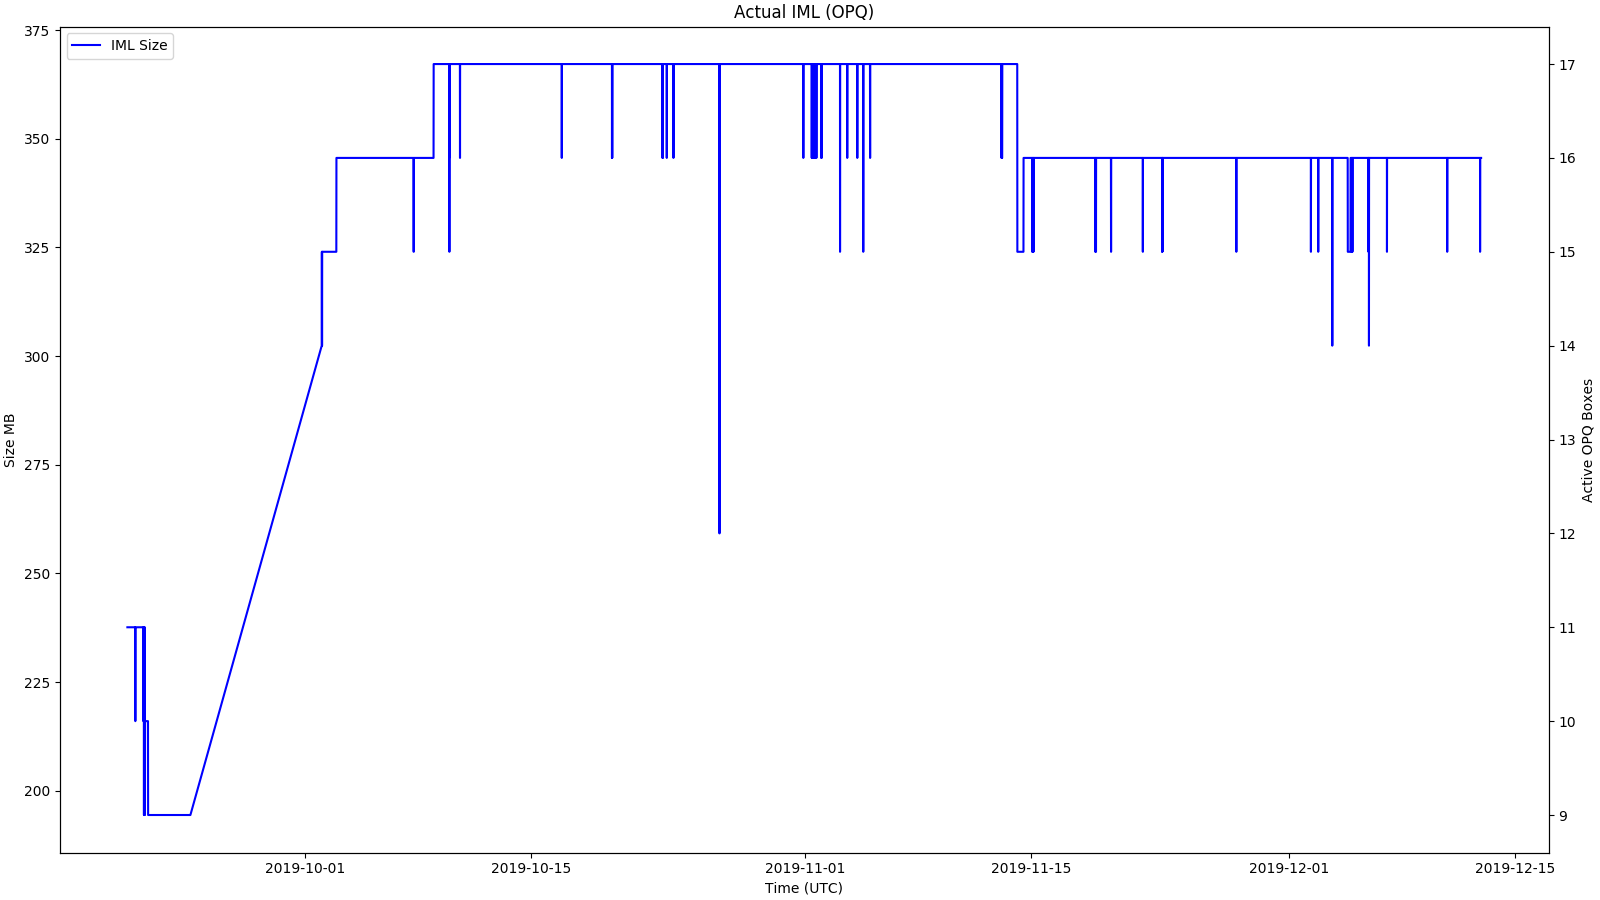
\includegraphics[width=\linewidth]{figures/actual_iml_opq.png}
    \caption{Actual IML for OPQ}
    \label{fig:actual_iml_opq}
\end{figure}

A deployment of 15 OPQ Boxes will consume about 325 MB of IML space. The changes in data size are attributed to the fact that OPQ Boxes came on and offline during the period of the OPQ deployment. At the lowest point, only 9 OPQ Boxes were sending and at the highest point 17 OPQ Boxes were sending data. Garbage collection doesn't take place in the traditional sense in the cloud at this level as the IML samples are stored on the OPQ Boxes and bounded by the available memory that each Box can store. This plot assumes that at each Box is storing 15 minutes worth of data in a circular buffer. The spikes in IML size are from data gaps in sensor data. Either the sensor was powered off or there were network connectivity issues.

I will compare this result to the theoretical results in following sections.

\subsubsection{DSN System Requirements OPQ: AML}

The Aggregate Measurements Level (AML) contains summary statistics of features extracted from the IML. OPQ contains two sub-levels within the AML (Measurements and Trends). Data within the AML can be saved by higher levels within Laha (DL, IL, and PL). If AML data is saved, it receives the TTL of the highest level that the data was saved by.

I examine the AML data growth for OPQ by looking at the data growth of Measurements, Trends, and the total AML. Figure~\ref{fig:actual_aml_opq} displays the AML growth for the OPQ network as well as statistics about garbage collection.

\begin{figure}[H]
    \centering
    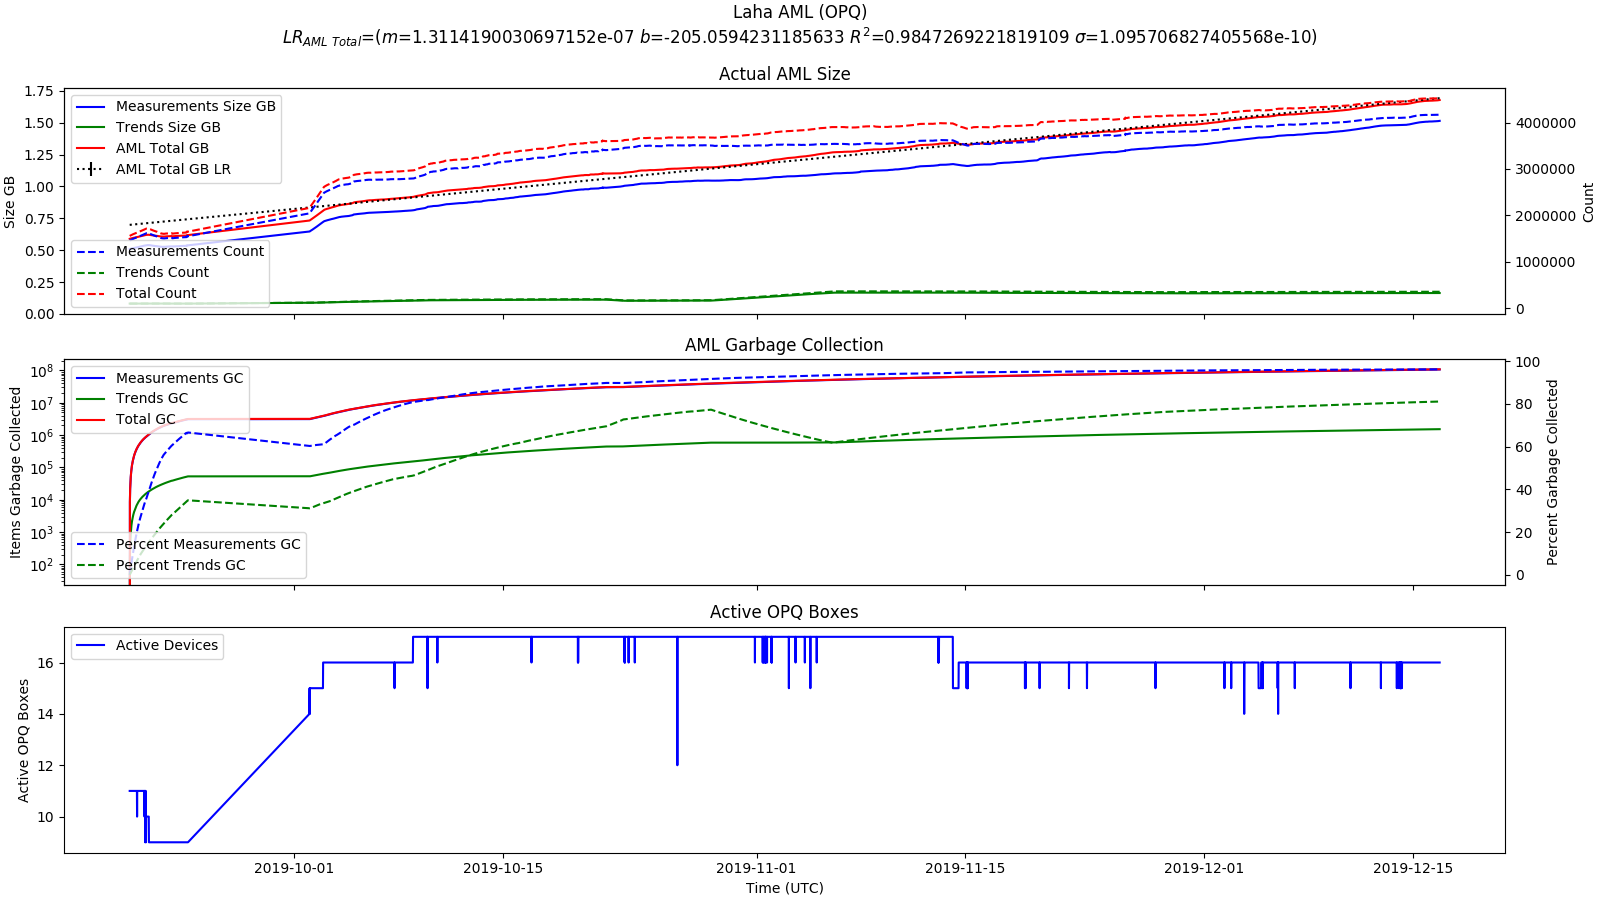
\includegraphics[width=\linewidth]{figures/actual_aml_opq.png}
    \caption{Actual AML for OPQ}
    \label{fig:actual_aml_opq}
\end{figure}

The top panel displays the AML data growth with size in GB on the left Y-axis and the count of AML items on the right Y-axis. Over a period of two and a half months the AML in OPQ has reached a size of about 1.75 GB containing over 4 million AML items.

The middle panel displays the number of Measurements and Trends that were garbage collected over time on the left Y-axis and the percentage of items that were garbage collected on the right Y-axis. About 98\% of all AML data was garbage collected. About 2\% of all AML data is either awaiting garbage collection or was ``saved" by a higher level in the Laha hierarchy.

The bottom panel displays the number of active OPQ Boxes over time. It's possible to see how the number of Boxes impacts the size of the AML. For example, the increase in Boxes in September and the decrease of Boxes in mid-November have noticeable impacts on the AML storage size.

I will compare this result to the theoretical results in following sections.

\subsubsection{DSN System Requirements OPQ: DL}

The Detections Level (DL) contains metadata and data bounded by a time window that may or may not contain signals of interest. Detections are generated by threshold based triggering algorithms. Detections can be saved by higher levels in the Laha hierarchy (IL and PL) and will receive the same TTL as the highest level the DL data is saved by. The DL contains metadata about the window it examines, but the bulk of data is produced by the raw samples that get copied into the DL when a Detection is created.

Figure~\ref{fig:actual_dl_opq} shows the DL data growth for the OPQ network over time.

\begin{figure}[H]
    \centering
    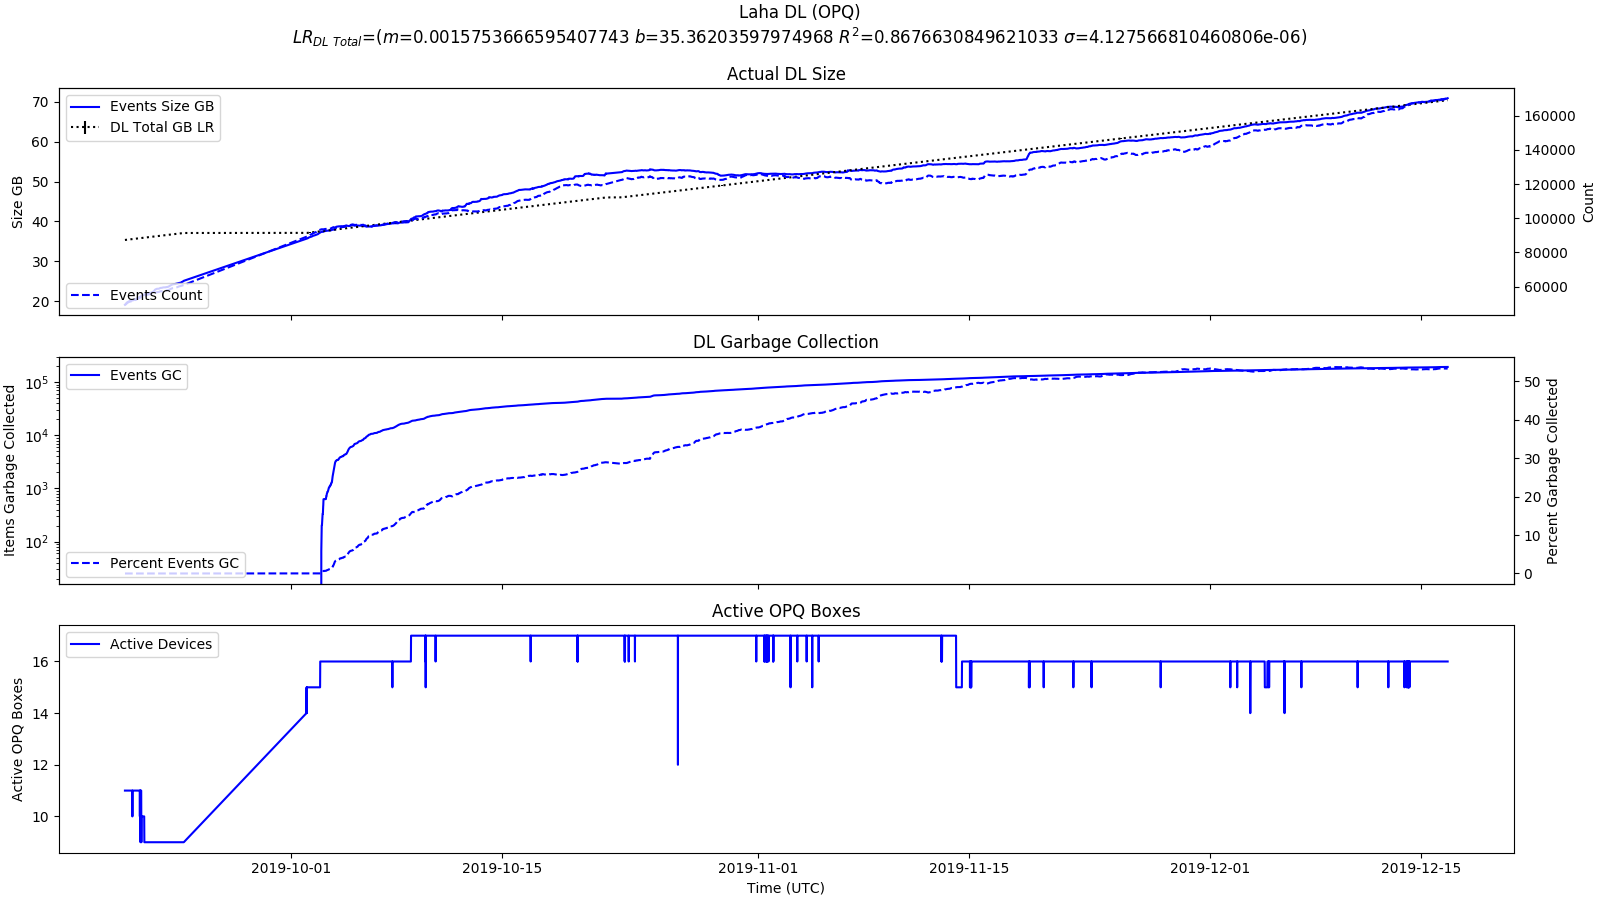
\includegraphics[width=\linewidth]{figures/actual_dl_opq.png}
    \caption{Actual DL for OPQ}
    \label{fig:actual_dl_opq}
\end{figure}

The top panel shows the size of the DL over time with the size in GB on the left Y-axis and the count of Detections on the right Y-axis. The size of the DL for the OPQ network has grown to close 70 GB over the period of two and half months containing a total of 160,000 Detections.

The middle panel shows the garbage collection statistics for the DL. Of note is the delayed uptick in garbage collection until October 1, 2019. This is a direct result of the fact that Detections have a TTL of 1 month, and thus, no Detections were garbage collected during the first month of data collection. As of two and a half months of data collection, about 50\% of all Detections generated have been garbage collected while the other 50\% are wither awaiting garbage collection or have been saved by Incidents or Phenomena.

The bottom panel shows the number of active OPQ Boxes sending data over time.

I will compare this result to the theoretical results in following sections.

\subsubsection{DSN System Requirements OPQ: IL}

The Incidents Level (IL) contains metadata and data relating to classified signals of interest. Incidents are created when a Mauka plugin classifies a signal of interest from a Detection. Incidents can be saved by Phenomena.

Figure~\ref{fig:actual_il_opq} shows the IL growth for the OPQ network over a period of two and a half months.

\begin{figure}[H]
    \centering
    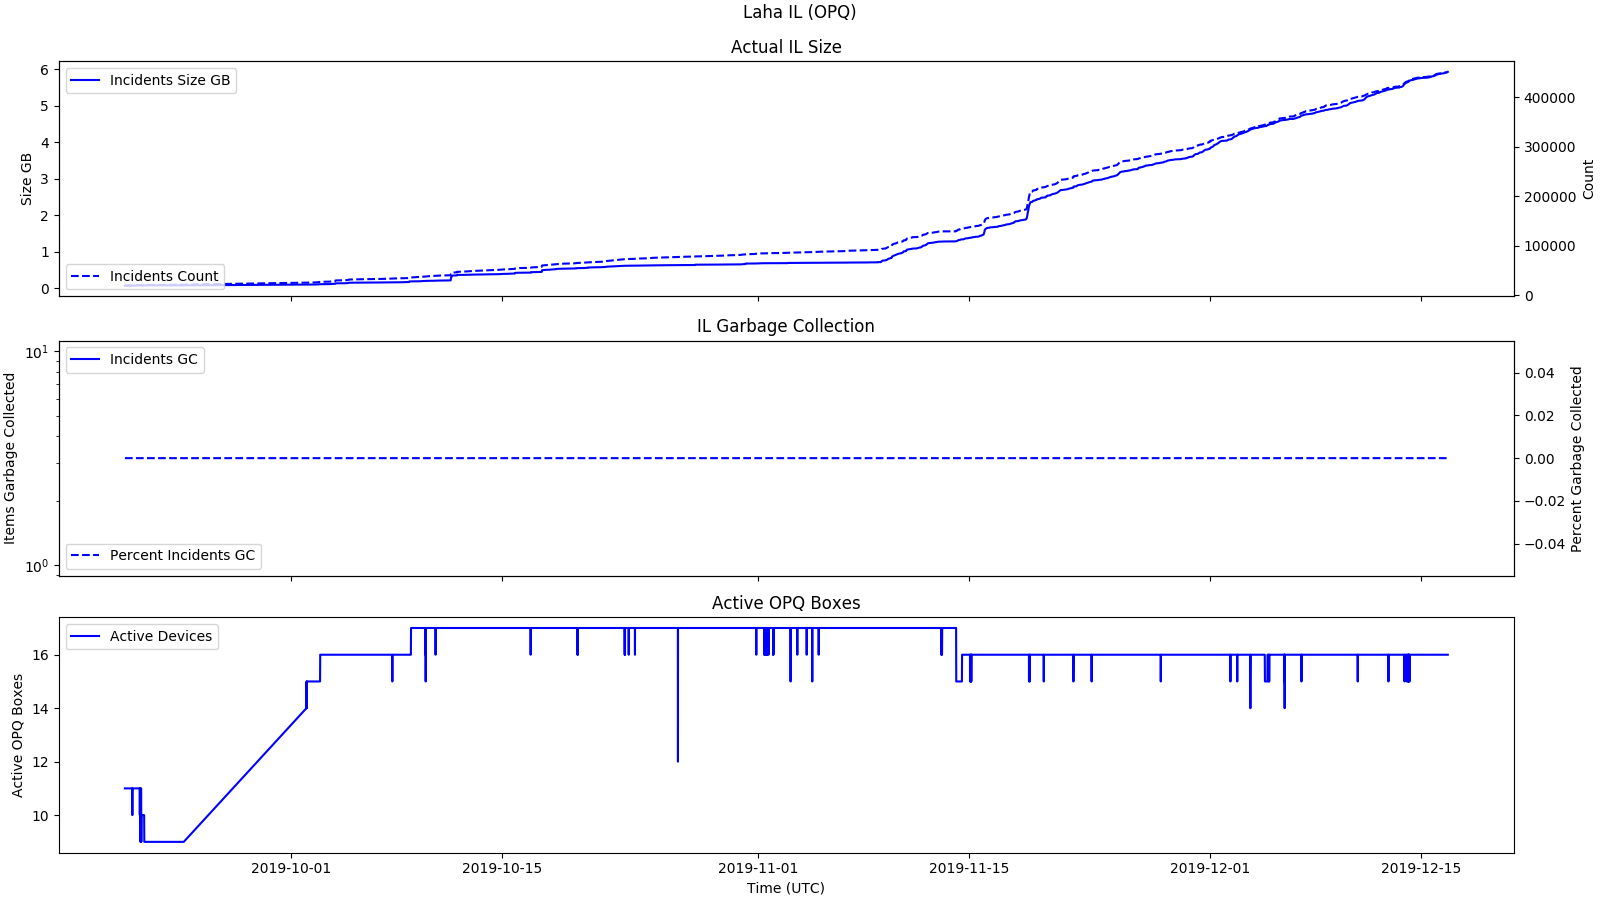
\includegraphics[width=\linewidth]{figures/actual_il_opq.png}
    \caption{Actual IL for OPQ}
    \label{fig:actual_il_opq}
\end{figure}

The top panel shows the growth of the IL with the size in GB on the left Y-axis and the number of Incidents on the right Y-axis. Over a period of two and a half months, the IL of OPQ has grown to near 6GB containing over 400,000 Incidents.

The middle panel shows the garbage collection statistics for the IL. You'll note that the GC statistics are flat lining at 0. This is due to the fact that Incidents are given a default TTL of 1 year and this deployment has only been collecting data for 3 months.

This brings up the question, is a TTL of 1 year for Incidents too long? It's clearly not useful over a deployment of 3 months, but DNSs utilizing Laha are expected to operate in a stable fashion for long durations. Incidents, only being one step below Phenomena, contain a wealth of information in the form of classified signals of interest. I believe that data that has been classified should live for a long time duration. Since Events live for a month and Phenomena live for a 2 years, it makes sense to me to have a TTL of 1 year for Incidents. One of the reasons I decided to simulate Laha in terms of data storage requirements was so that I could show expected results for time periods larger than that of the OPQ deployment. We could scale back the TTL of Incidents to 6 months, but this would still be beyond the range of the OPQ deployment duration. Future work on Laha will examine how altering TTLs of the various levels affect the underlying data storage characteristics.

The bottom panel shows the number of active OPQ Boxes sending data over time.

I will compare this result to the theoretical results in following sections.

\subsubsection{DSN System Requirements OPQ: PL}

% TODO
TODO

\subsubsection{DSN System Requirements OPQ}

I will now examine the results of combining all Laha levels within OPQ. Figure~\ref{fig:actual_laha_opq} provides the results of data collection for the entire OPQ network over a period of 2 and a half months.

\begin{figure}[H]
    \centering
    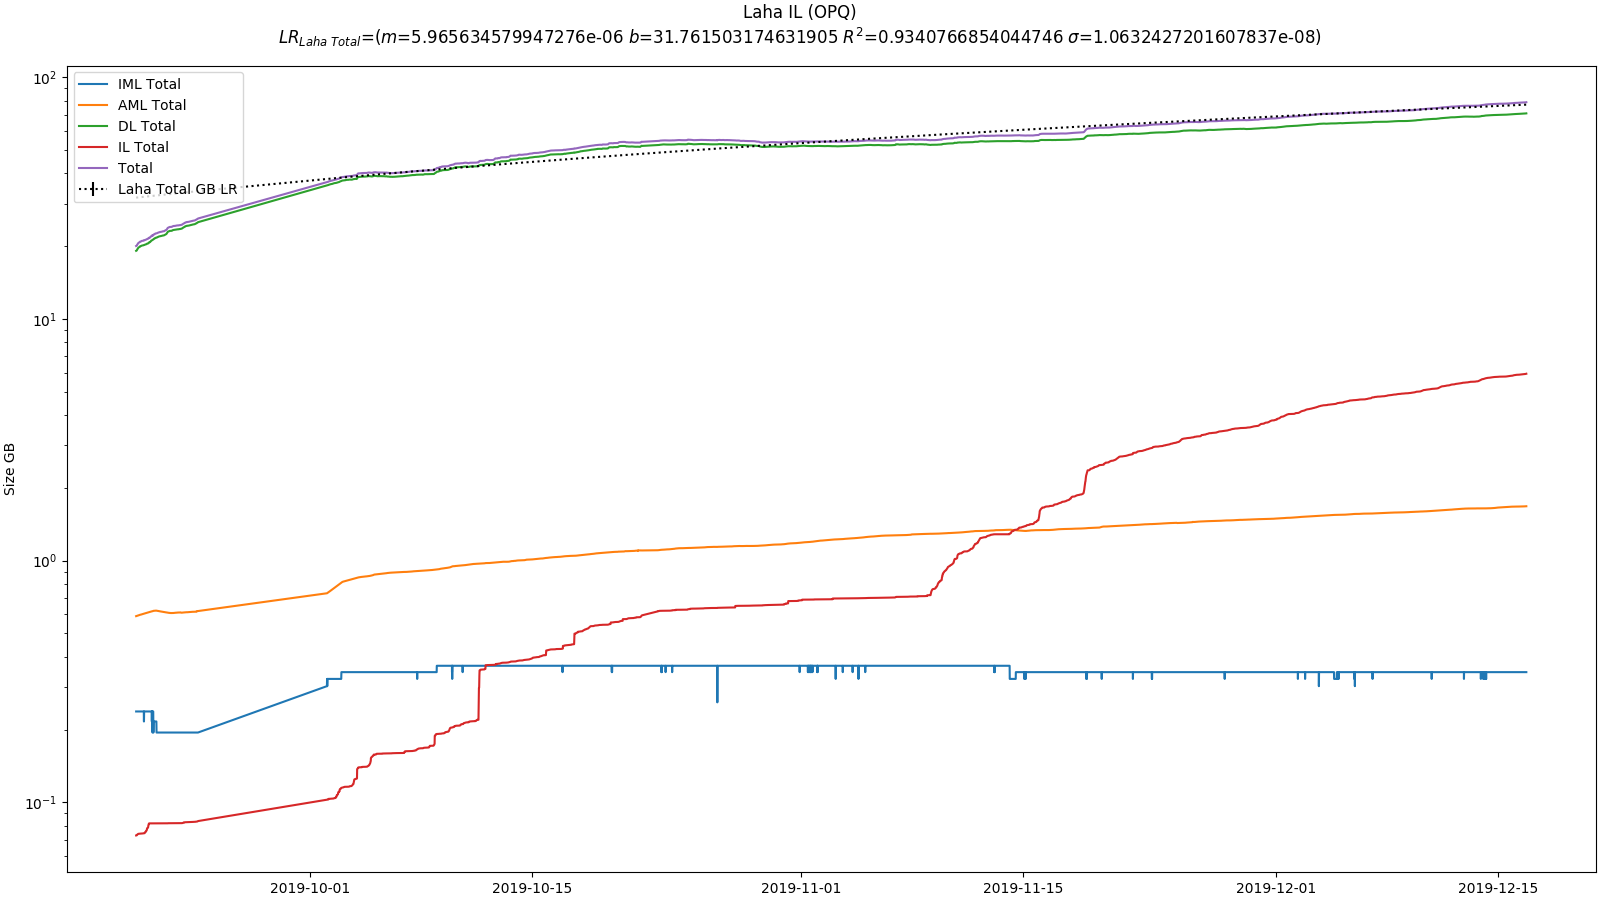
\includegraphics[width=\linewidth]{figures/actual_laha_opq.png}
    \caption{Actual Laha for OPQ}
    \label{fig:actual_laha_opq}
\end{figure}

First, please note that the Y-axis is using a log scale in order to better display the data growth of some of the smaller Laha levels. Next, we observe that the size of the entire network is just under 100 GB over a period of two and a half months with an average of 15 OPQ Boxes.

We can observe that the IML level converges to the smallest of the levels due to its strict 15 minute TTL.

The IL starts out small, but as Incidents are identified, the IL surpasses the IML at about 1 month and surpasses the AML in size at about 2 months. The Detections level is the largest and this makes sense since we treat Detections relatively cheaply and they contain windows of data that are generally larger than the signal of interest if there even is a signal of interest at all.

I will compare this result to the theoretical results in following sections.

\subsubsection{DSN System Requirements OPQ: Comparing Results to Estimates}

Now that I have shown the results for the actual DSN storage requirements, I will next compare these results to the estimated storage requirements with and without TTL\@.

Let us first compare the results to the estimated storage requirements without TTL found in Section~\ref{sssec:eval_of_dsn_system_requirements}. This might feel a bit contrived, but the purpose of these results is to show how OPQ compares to a similar system that would collect everything.

One interesting thing to note is that I expected the estimated values to be much higher than the actual values due to the fact that I was not including TTL explicitly anywhere in the estimations. It turns out this is not always the case. The reason for this is that the estimated values are computed by multiplying the amount of time the system has been running with the data rate obtained from the OPQ database for Events, Incidents, and Phenomena, and on the surface, it does not appear that TTL is being used in these estimations. However, this is not exactly the case. The data rate parameters obtained from the OPQ database implicitly have the TTL built in. That is because I measure the data rate over all available Events, Incidents, and Phenomena, but this data rate does not include Incidents, Events, or Phenomena that have been garbage collected! Unfortunately, I do not have detailed metrics on data that was garbage collected (only counts). Any future DSN utilizing Laha should consider recording detailed metrics about data that was garbage collected (duration, data stored, etc).

This really only affects Detections, Incidents, and Phenomena which use estimated database parameters. Samples, Measurements, and Trends are not affected because they are computed directly from the time length without using any estimated database parameters.

The end result of this is that it turns out that the method I use to estimate Events, Incidents, and Phenomena without TTL pretty accurately portray the size of the actual data with TTL.

There was already data in the database before we started collected enhanced metrics. This is true for the AML, DL, IL, and PL. In order to accurately compare data growths from zero, the first value at each level is subtracted from the entire data set at each level. This essentially ``forces" the data set to start at 0 so that we can compare it directly to the estimates.

\paragraph{IML Versus Estimated Growth}
The Instantaneous Measurements Level (IML) consists of raw samples from sensors. Figure~\ref{fig:actual_iml_vs_unbounded_opq} shows the actual IML vs unbounded IML\@.

\begin{figure}[H]
    \centering
    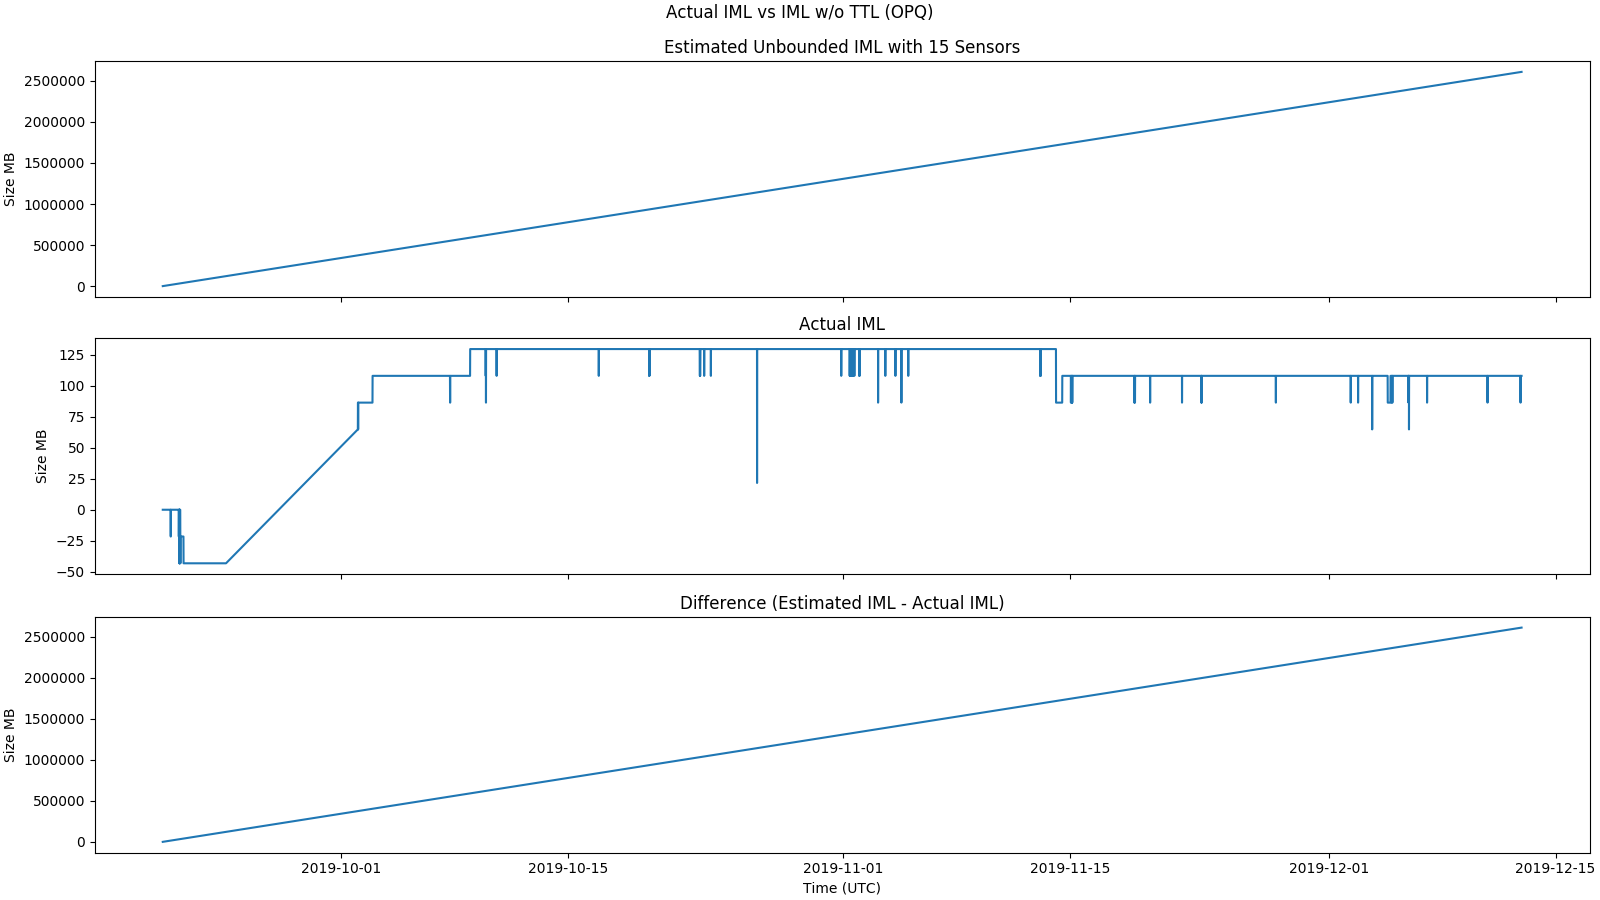
\includegraphics[width=\linewidth]{figures/actual_iml_vs_unbounded_opq.png}
    \caption{Actual IML vs Unbounded IML for OPQ}
    \label{fig:actual_iml_vs_unbounded_opq}
\end{figure}

This plot is a little uninteresting. The difference is lost by the shear imbalance between magnitudes. With the IML producing the most data consisting of raw samples, without a TTL of 15 minutes the unbounded IML grows very quickly. By having bounds on the data, OPQ saves over 2.5 TB worth of data storage.

\paragraph{AML Versus Estimated Growth}
Figure~\ref{fig:actual_aml_vs_unbounded_opq} shows the actual AML vs unbounded AML. The AML level contains aggregate measurements which are rolled up summary statistics extracted from the IML\@.

\begin{figure}[H]
    \centering
    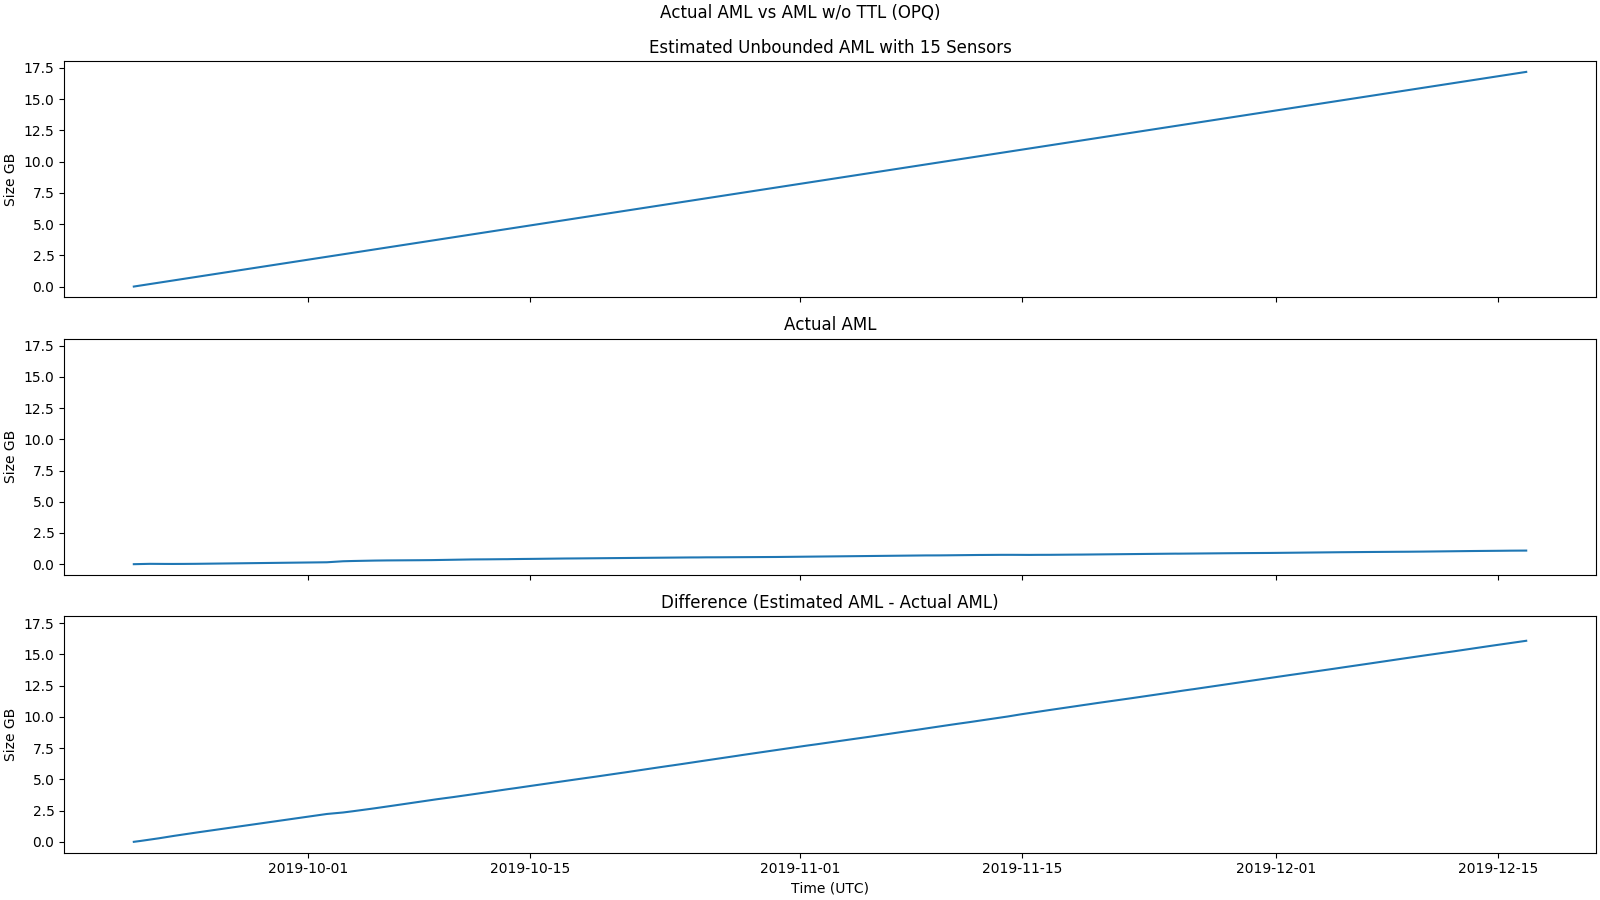
\includegraphics[width=\linewidth]{figures/actual_aml_vs_unbounded_opq.png}
    \caption{Actual AML vs Unbounded AML for OPQ}
    \label{fig:actual_aml_vs_unbounded_opq}
\end{figure}

This data was not affected by the implicit TTL parameter and portrays accurate unbounded versus bounded growth. We can see that over the same time period, AML with TTL saved us about 17.5 GB worth of data versus a store everything approach.

\paragraph{DL Versus Estimated Growth}
Figure~\ref{fig:actual_dl_vs_unbounded_opq} shows the actual DL vs unbounded DL. The Detection Level contains metadata and data bounded by a window which may or may not include signals of interest.

\begin{figure}[H]
    \centering
    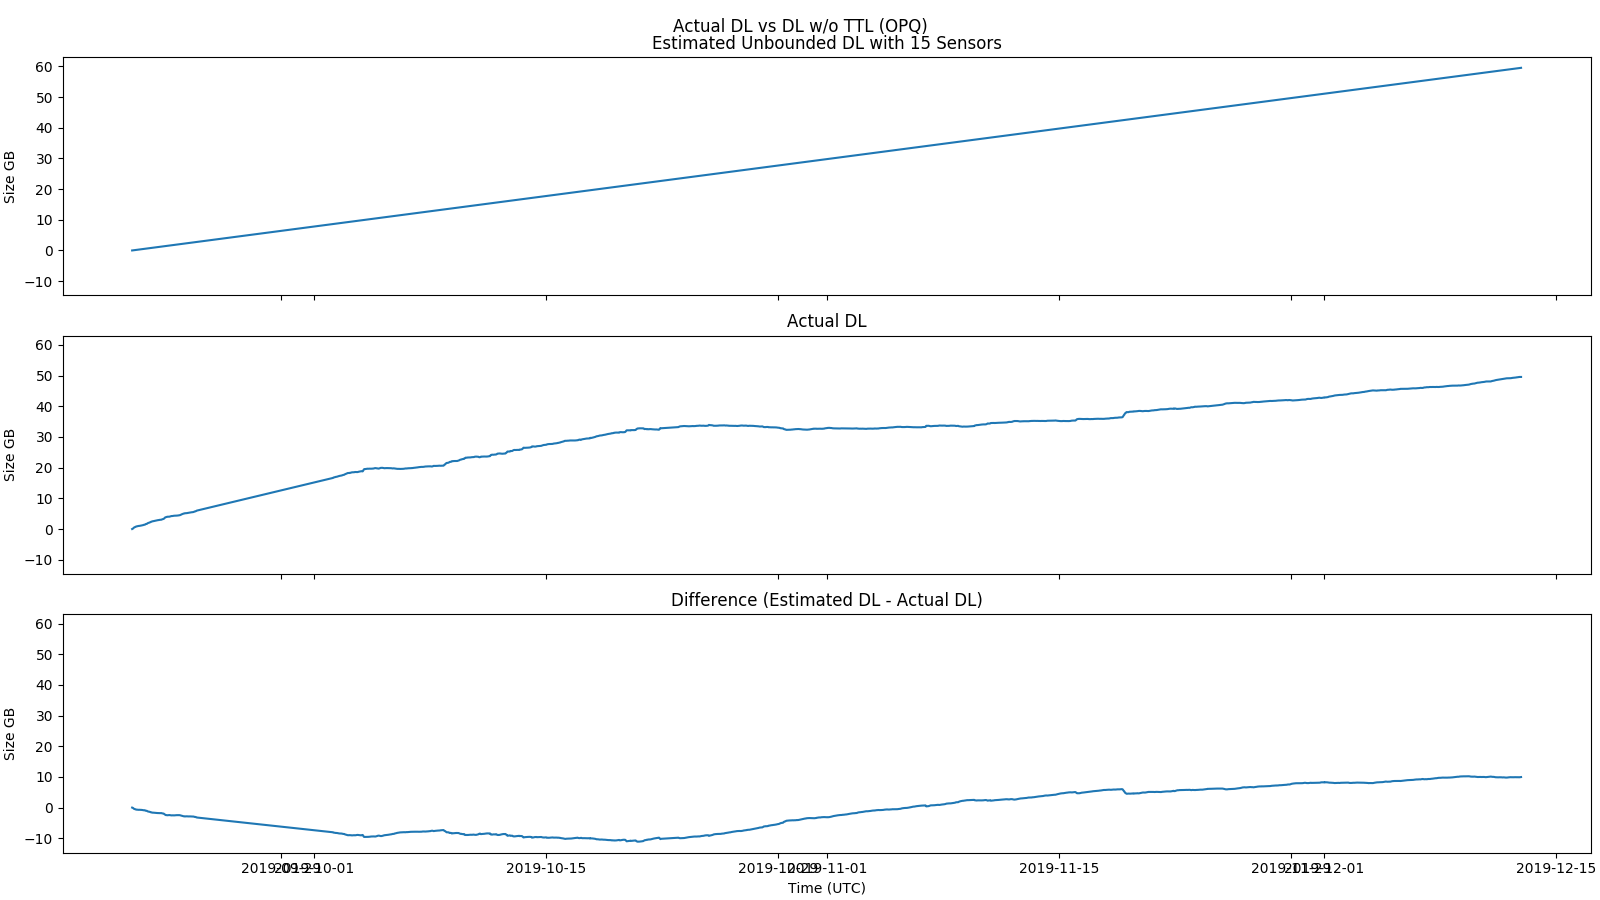
\includegraphics[width=\linewidth]{figures/actual_dl_vs_unbounded_opq.png}
    \caption{Actual DL vs Unbounded DL for OPQ}
    \label{fig:actual_dl_vs_unbounded_opq}
\end{figure}

This data was affected by the implicit TTL parameter and does not portray accurate unbounded versus bounded growth. Instead, the implicit TTL parameter models are actual growth pretty closely and the actual data is about 20 GB larger than the estimated data growth.

\paragraph{IL Versus Estimated Growth}
Figure~\ref{fig:actual_il_vs_unbounded_opq} shows the actual IL vs unbounded IL. The Incident Level contains metadata and data over window that contains classified signals of interest.

\begin{figure}[H]
    \centering
    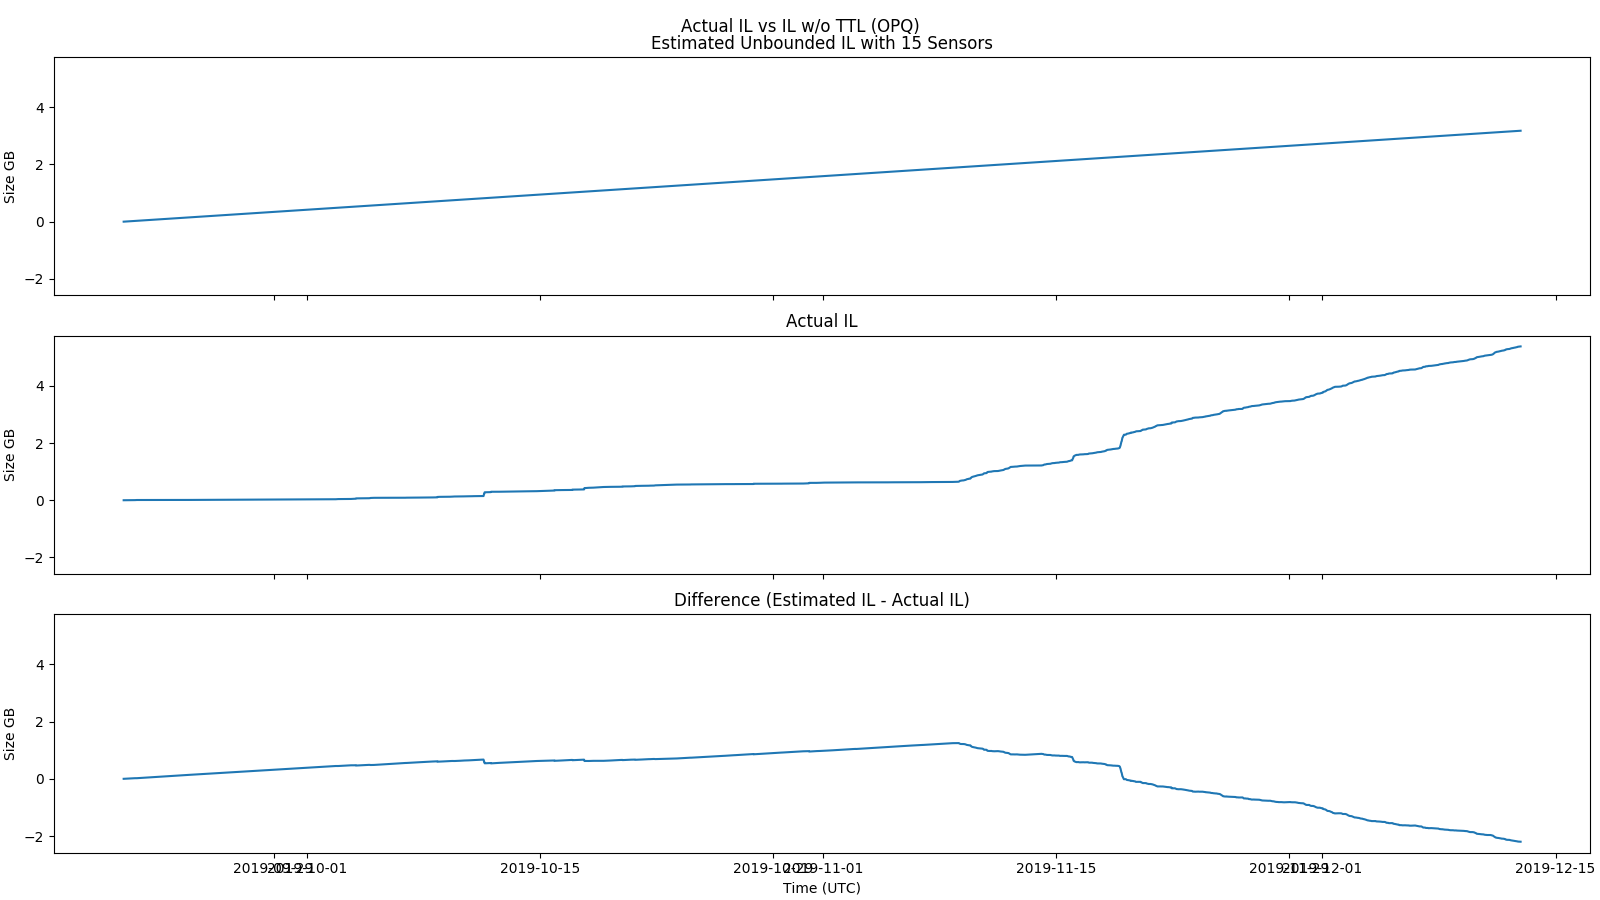
\includegraphics[width=\linewidth]{figures/actual_il_vs_unbounded_opq.png}
    \caption{Actual IL vs Unbounded IL for OPQ}
    \label{fig:actual_il_vs_unbounded_opq}
\end{figure}

This data was affected by the implicit TTL parameter and does not portray accurate unbounded versus bounded growth. Instead, we can see that the actual size of the IL tracks pretty closely to the estimated maximum bounds. At the end of the data collection period, OPQ collected about 4GB less worth of data than what was estimated.

\paragraph{PL Versus Estimated Growth}
Figure shows the actual PL vs unbounded PL.

% TODO
TODO

\paragraph{Laha Versus Estimated Growth}
Finally, I examine the total size of Laha and compare it to the estimated bounds of Laha without TTL. This takes into account all levels within the Laha hierarchy.

Figure~\ref{fig:actual_laha_vs_unbounded_opq} compares the actual bounds of the entire network to the estimated bounds.

\begin{figure}[H]
    \centering
    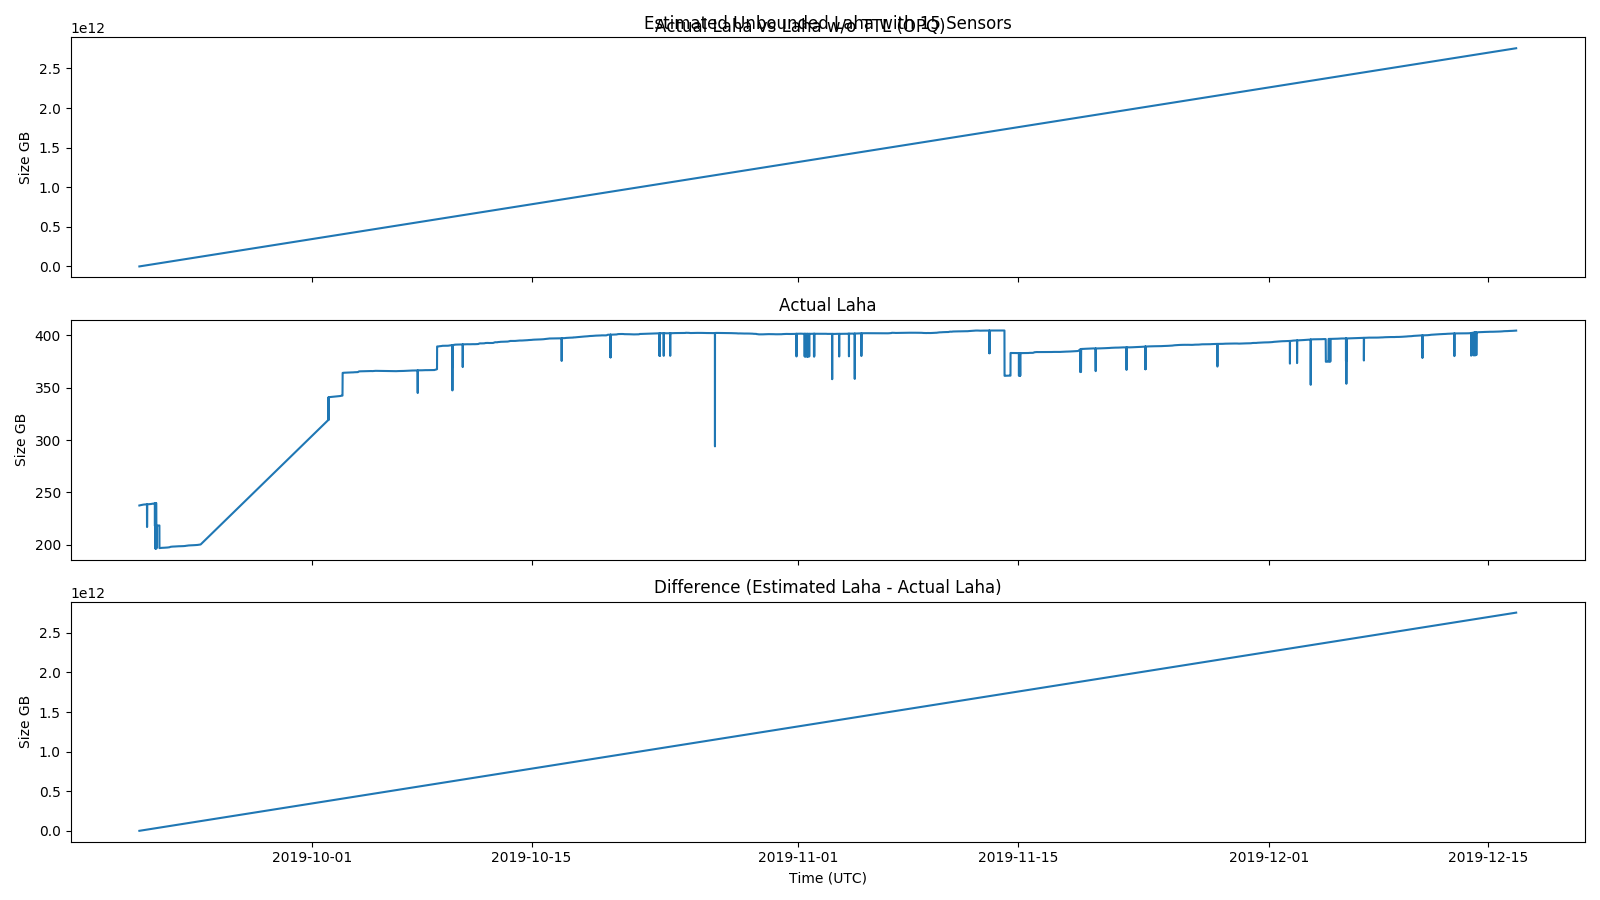
\includegraphics[width=\linewidth]{figures/actual_laha_vs_unbounded_opq.png}
    \caption{Actual Laha vs Unbounded Laha for OPQ}
    \label{fig:actual_laha_vs_unbounded_opq}
\end{figure}

This result is a little unsatisfying. The data growth of the IML is pretty much the only feature evident in this plot. To better understand the growth of the entire system, I removed the IML as shown in Figure~\ref{fig:actual_laha_vs_unbounded_no_iml_opq}.

\begin{figure}[H]
    \centering
    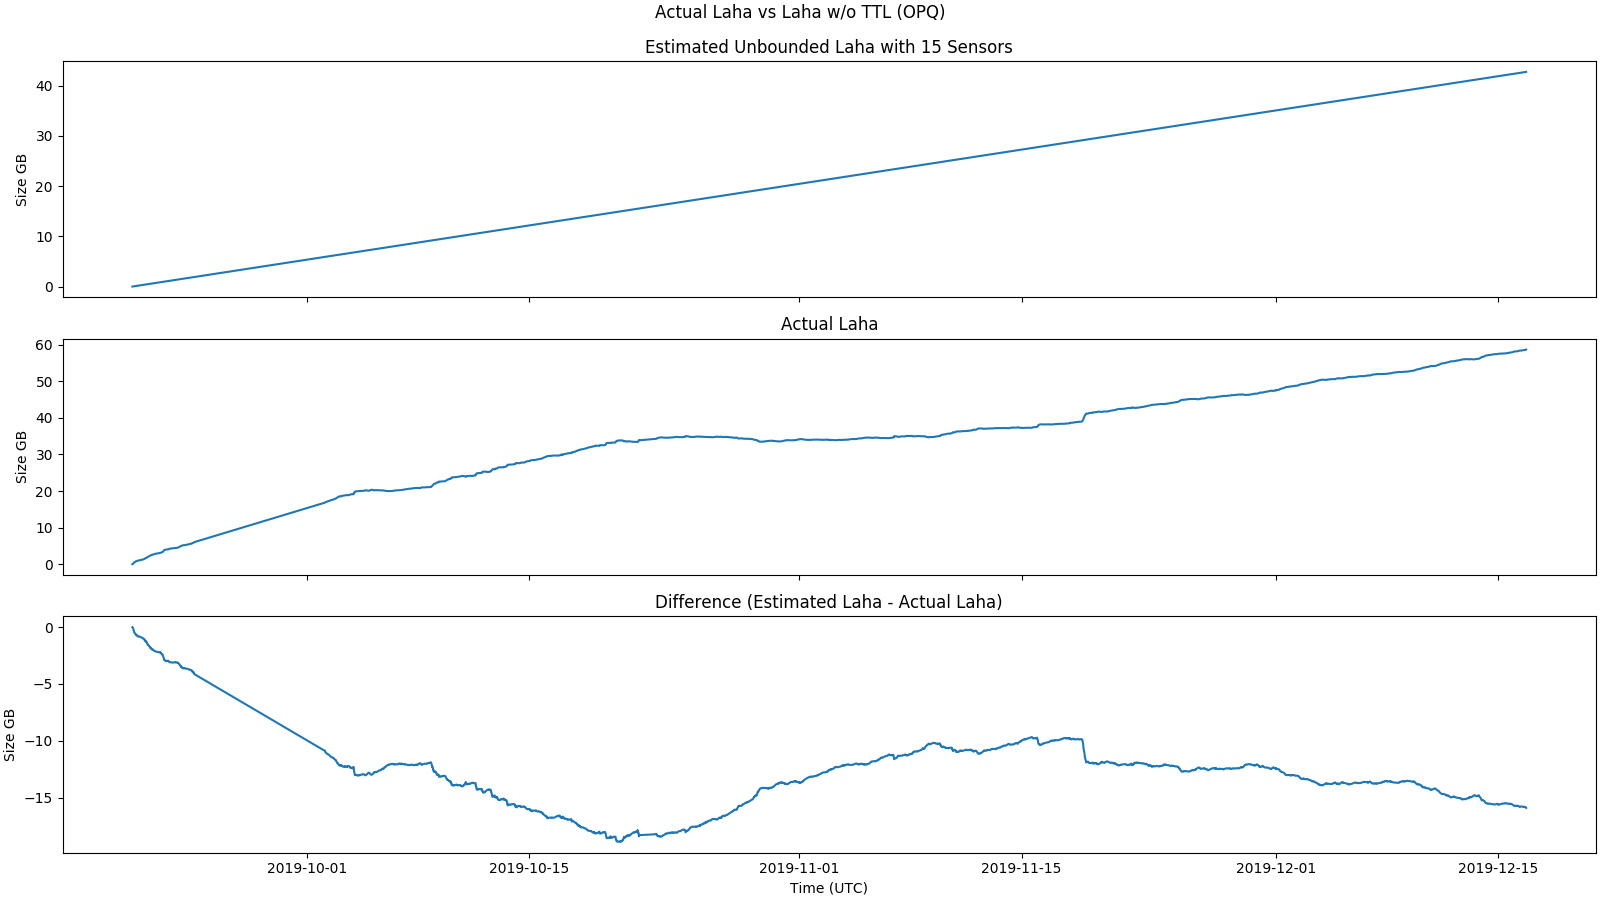
\includegraphics[width=\linewidth]{figures/actual_laha_vs_unbounded_opq_no_iml.png}
    \caption{Actual Laha vs Unbounded Laha for OPQ (No IML)}
    \label{fig:actual_laha_vs_unbounded_no_iml_opq}
\end{figure}

Over a time period of 2 and a half months, the OPQ network saved about 20GB of data as compared to a store everything approach (not including the IML which saved about 2.5 TB of data). Of course, I would expect this difference to be greater if I had actual metrics for the DL, IL and PL that did not have a built-in implicit TTL parameter. Even with the built-in parameter, the savings gained from the AML alone is significant.

\subsubsection{DSN System Requirements OPQ: Comparing Results to Simulated Data}

Next I will compare the results gathered from the OPQ deployment to the simulated bounds found in Section~\ref{sssec:evaluation_of_ttl}.

Similar to the previous comparisons, I will offset the actual data to ``force" the data to start from zero.

The simulated data had to be aligned with the collected metrics to perform this evaluation. The alignment works by binning all relevant timestamps to the nearest minute between the two data series.

\paragraph{IML Versus Simulated Growth}
The Instantaneous Measurements Level (IML) contains raw samples from sensors. Figure~\ref{fig:actual_iml_vs_sim_opq} shows the actual IML vs estimated IML.

\begin{figure}[H]
    \centering
    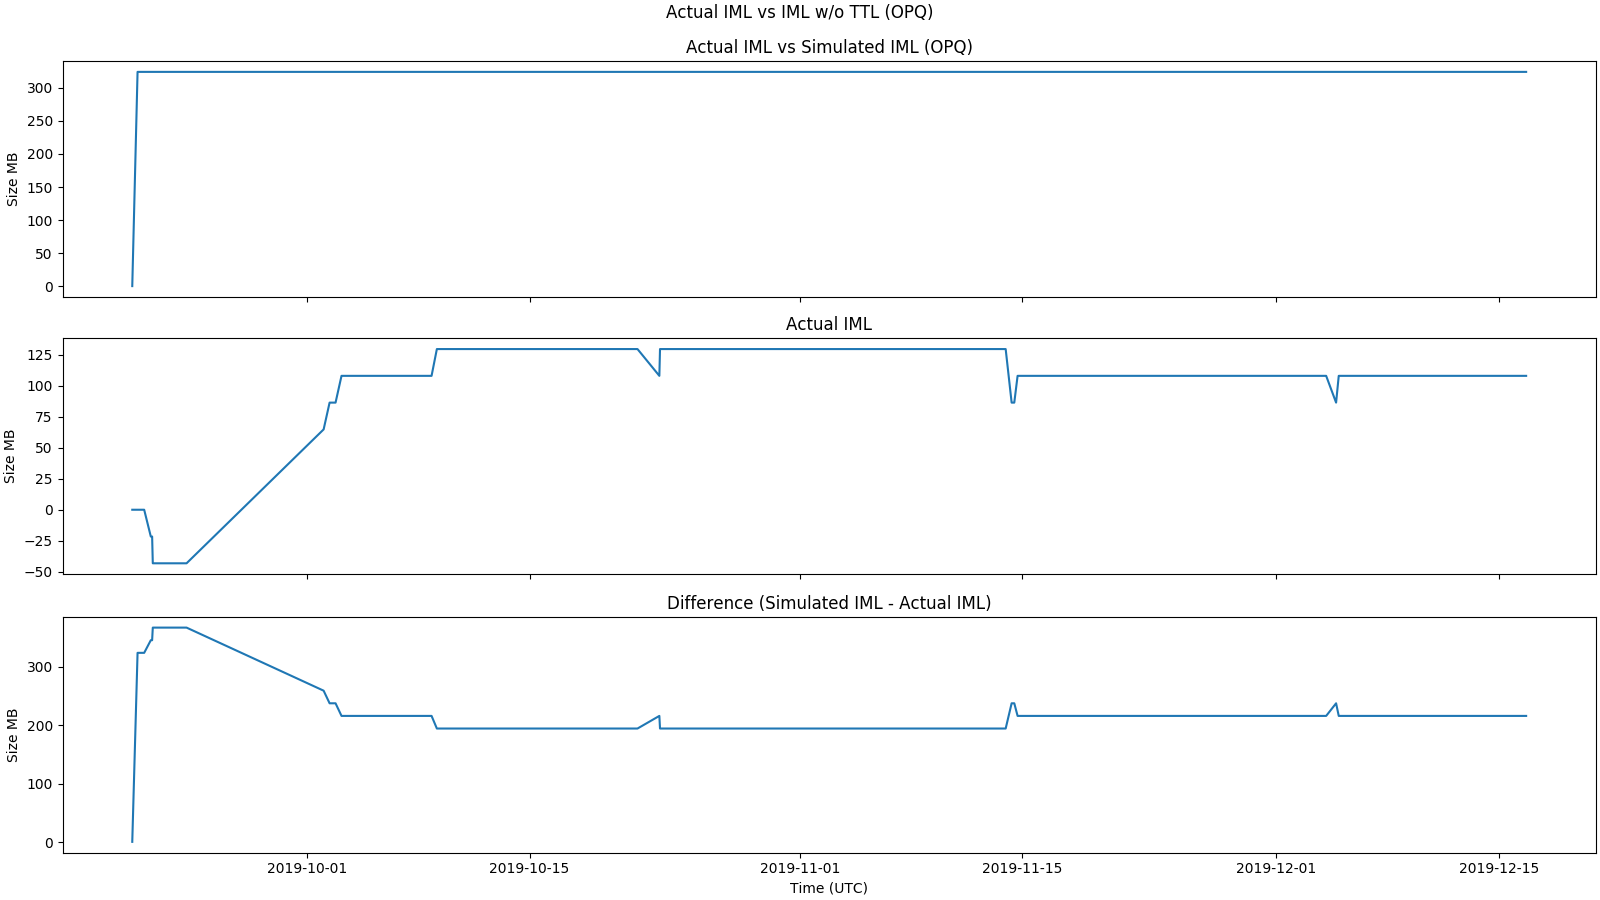
\includegraphics[width=\linewidth]{figures/actual_iml_vs_sim_opq.png}
    \caption{Actual IML vs Simulation IML for OPQ}
    \label{fig:actual_iml_vs_sim_opq}
\end{figure}

The simulation tracks the actual data pretty closely with a difference hovering around 0 MB. The simulation assumes that 15 sensors are always sending, whereas the actual data fluctuates with the number of active sensors.

\paragraph{AML Versus Simulated Growth}
The Aggregate Measurements Level (AML) contains rolled up summary statistics of selected features generated from IML data. Figure~\ref{fig:actual_aml_vs_sim_opq} shows the actual AML vs estimated AML.

\begin{figure}[H]
    \centering
    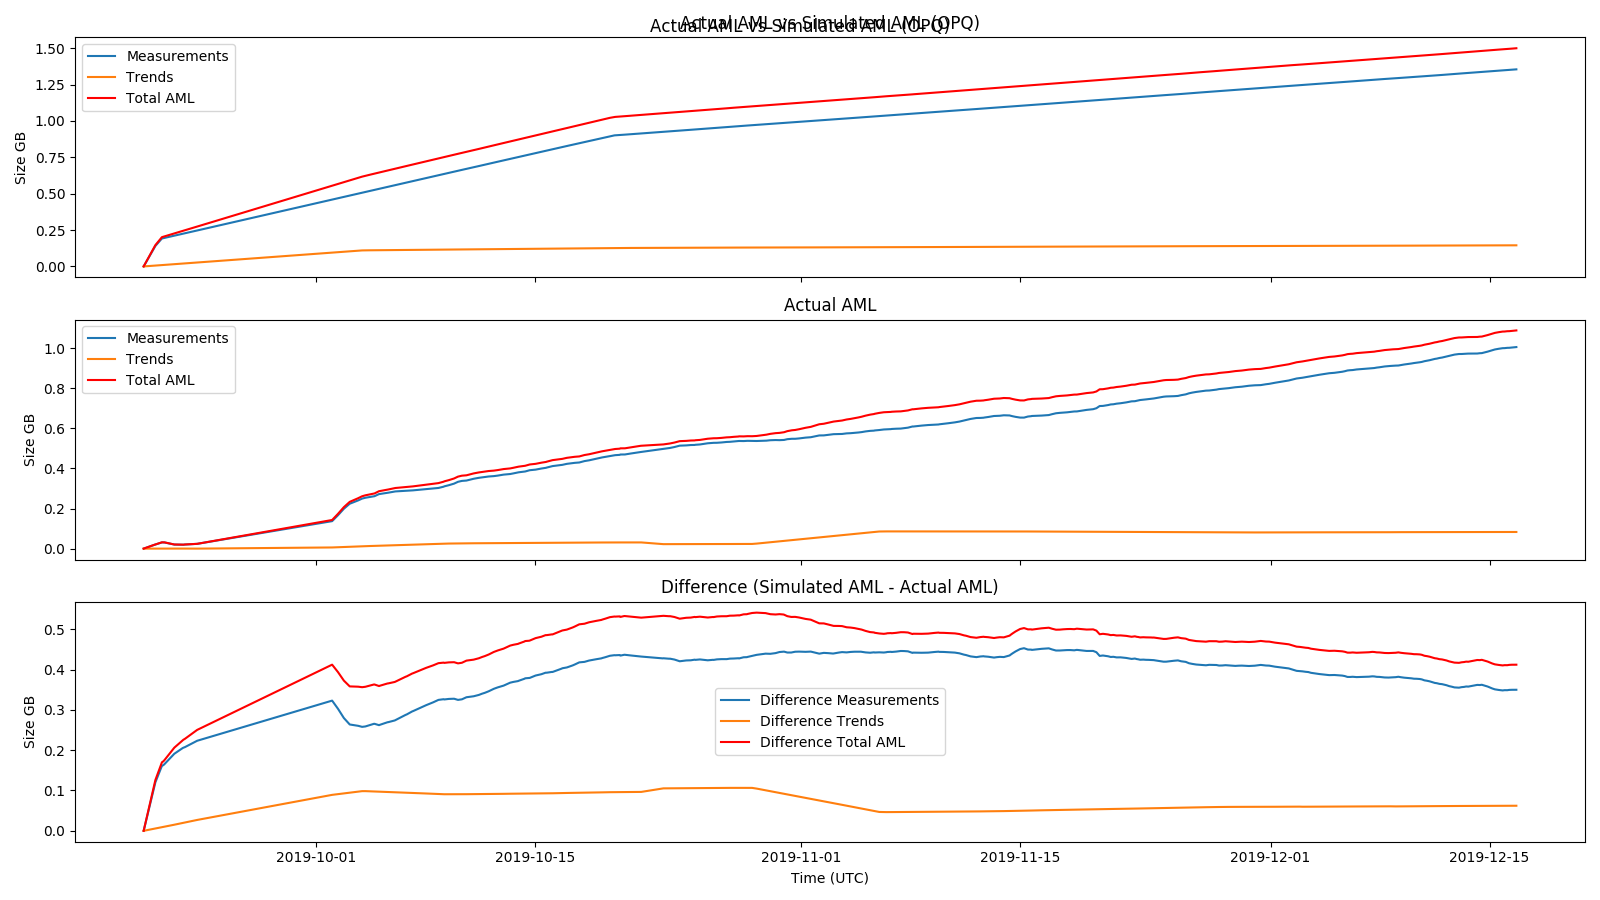
\includegraphics[width=\linewidth]{figures/actual_aml_vs_sim_opq.png}
    \caption{Actual AML vs Simulation AML for OPQ}
    \label{fig:actual_aml_vs_sim_opq}
\end{figure}

The simulated AML data trends closely with the actual data. There is a slight underestimation early on, but converges to close to 0 GB by the end of the data collection.

\paragraph{DL Versus Simulated Growth}
The Detection Level (DL) contains metadata and a window of raw data that may or may not include signals of interest. Figure~\ref{fig:actual_dl_vs_sim_opq} shows the actual DL vs estimated DL.

\begin{figure}[H]
    \centering
    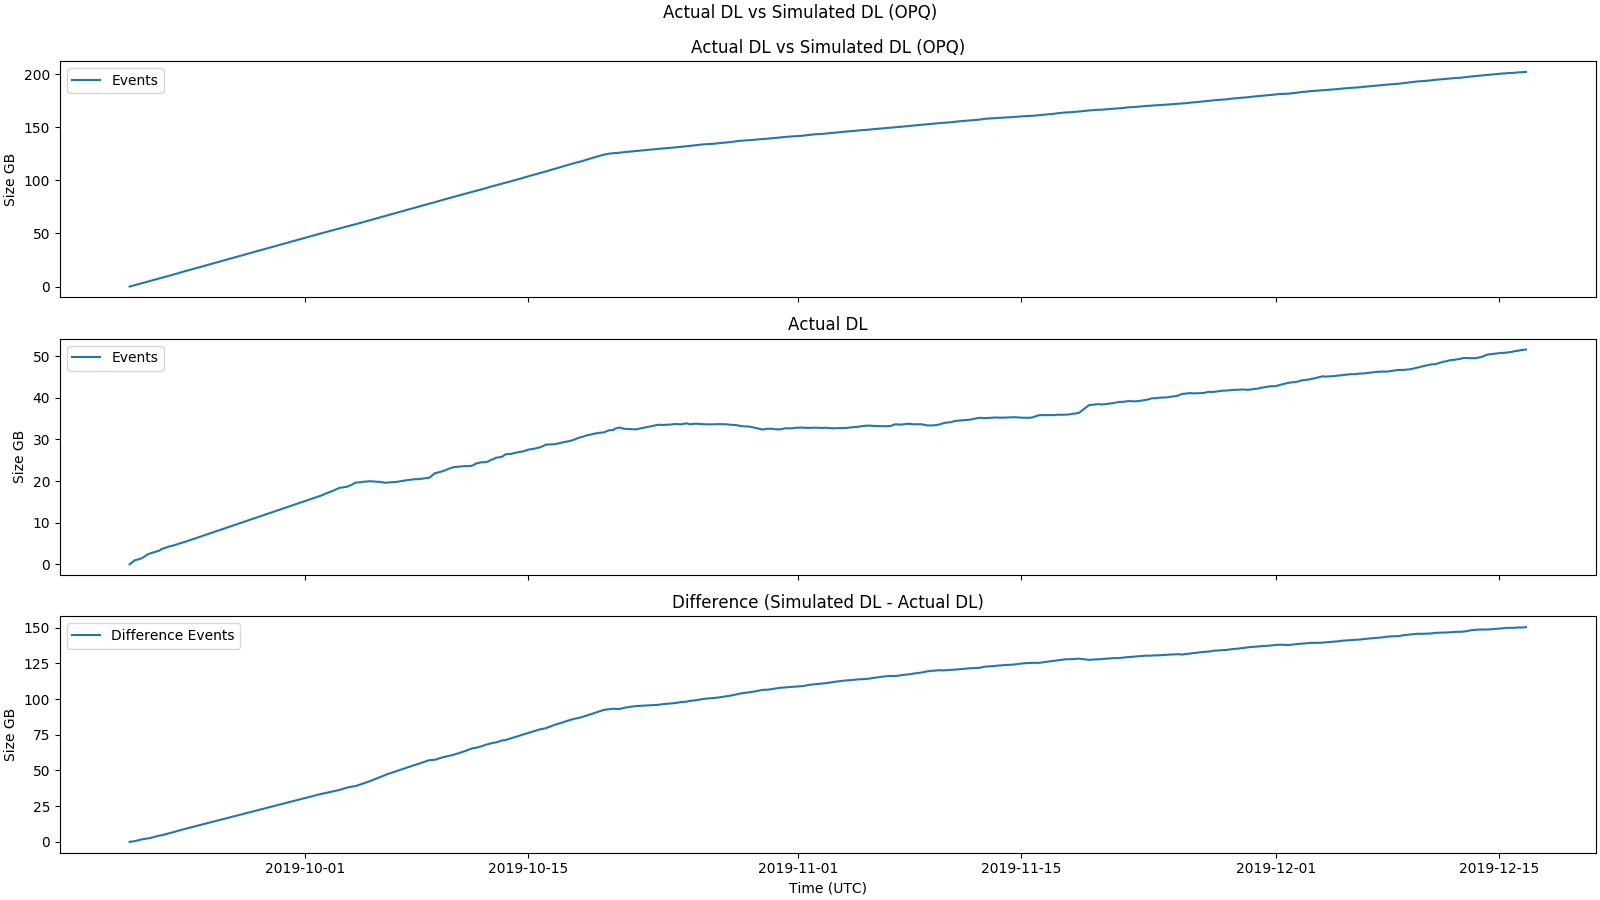
\includegraphics[width=\linewidth]{figures/actual_dl_vs_sim_opq.png}
    \caption{Actual DL vs Simulation DL for OPQ}
    \label{fig:actual_dl_vs_sim_opq}
\end{figure}

Although the simulated data has a similar shape to the actual data for the DL, there is a large offset between the simulation and the actual data. There are several reasons for this offset. The parameters passed into the simulation have somewhat large variances. The leading issue though, is that the simulation assumes that each device produces the same amount of Detections. In practice, certain boxes produce many Detections while others produce relatively few Detections. These differences can likely be attributed to the offset. On the bright side, at least the actual data is less than the simulated data and not the other way around!

OPQ saves near 150 GB of data as compared to the simulation.

\paragraph{IL Versus Simulated Growth}
The Incidents Level (IL) contains metadata and a window of data that contains classified signals of interest. Figure~\ref{fig:actual_il_vs_sim_opq} shows the actual IL vs estimated IL.

\begin{figure}[H]
    \centering
    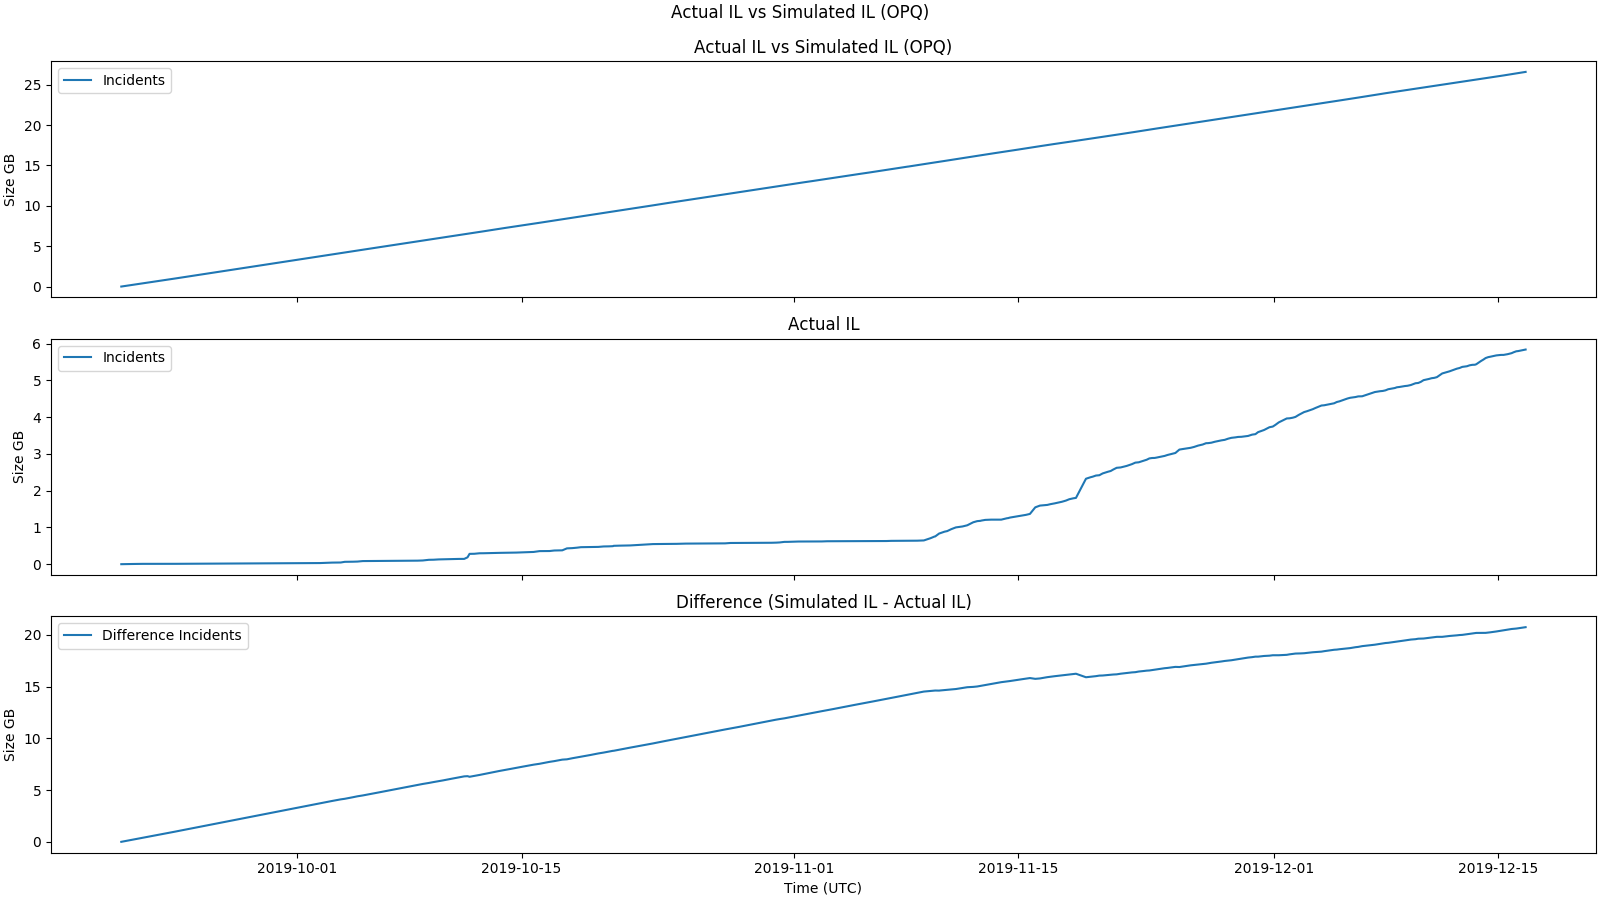
\includegraphics[width=\linewidth]{figures/actual_il_vs_sim_opq.png}
    \caption{Actual IL vs Simulation IL for OPQ}
    \label{fig:actual_il_vs_sim_opq}
\end{figure}

The simulated IL data is better than the simulated DL data, but still displays an offset, likely for the same reasons as the DL. OPQ saves 20 GB in the IL compared to the simulated IL.

\paragraph{PL Versus Simulated Growth}
Figure shows the actual PL vs estimated PL.

% TODO
TODO

\paragraph{Laha Versus Simulated Growth}
Figure~\ref{fig:actual_laha_vs_sim_opq} shows the actual Laha vs estimated Laha.

The large offsets in the simulated DL and IL data create the overall trends in this plot. The shapes of the trends are similar but the offset shows that OPQ saves near 150 GB of data over the same time period as the simulation.

\begin{figure}[H]
    \centering
    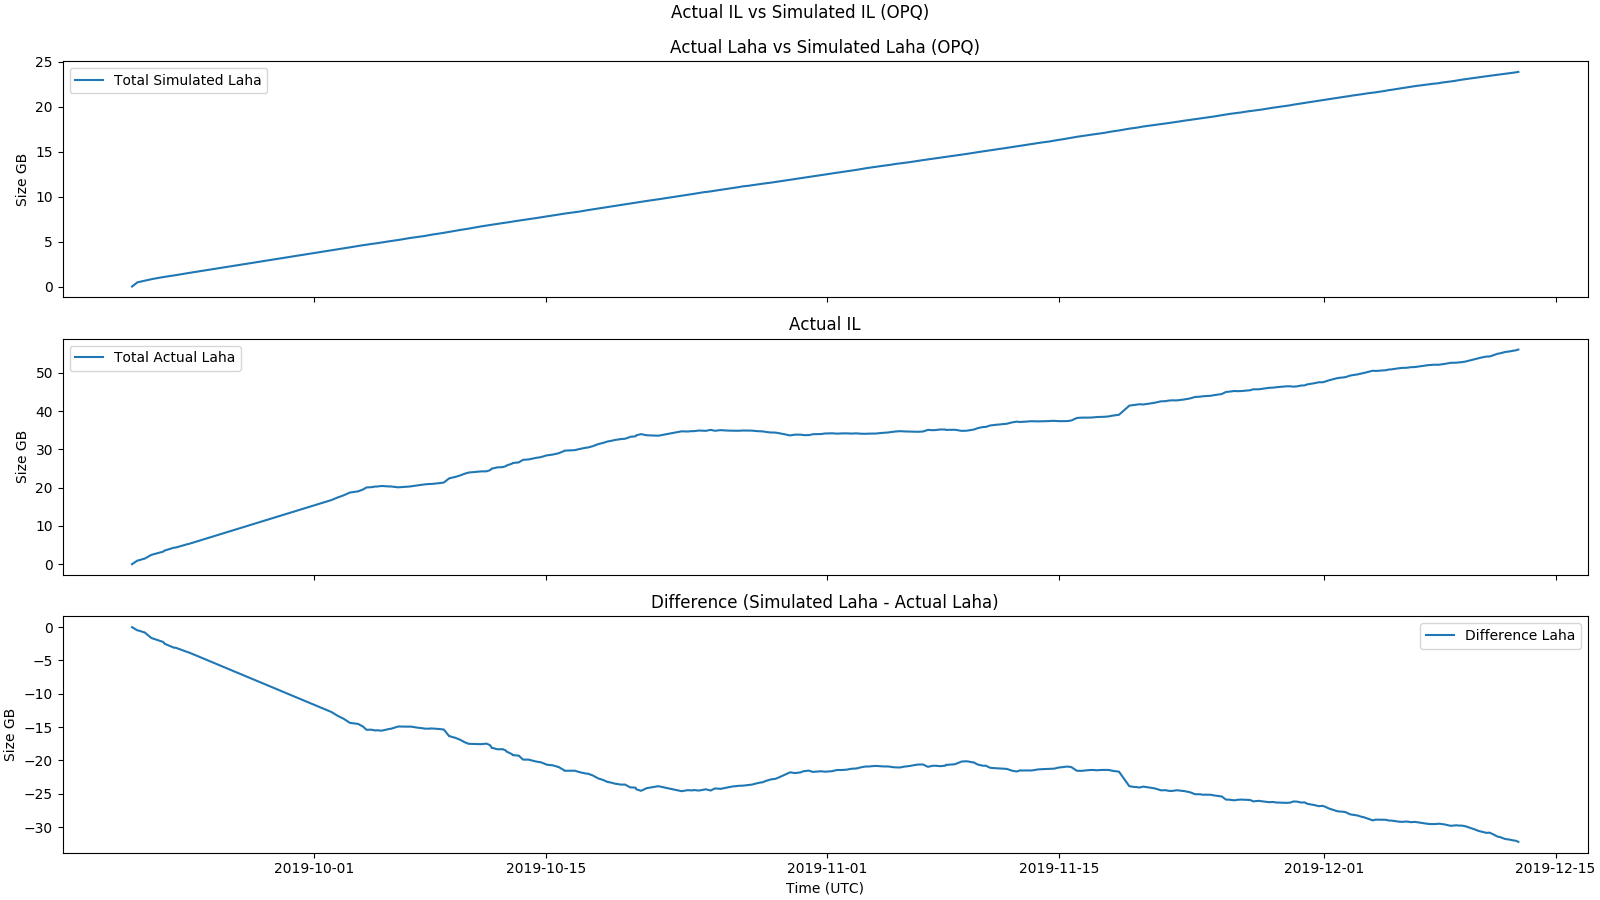
\includegraphics[width=\linewidth]{figures/actual_laha_vs_sim_opq.png}
    \caption{Actual Laha vs Simulation Laha for OPQ}
    \label{fig:actual_laha_vs_sim_opq}
\end{figure}

\paragraph{Discussion on Estimation Versus Simulation}

I compared actual data for each level in the Laha hierarchy to both estimated bounds and simulated bounds. Both approaches show promising results for certain levels. The estimated bounds are better suited for examining the DL, IL, and PL whereas the simulated bounds are better for examining the IML and AML. The estimated bounds include an implicit TTL parameter where the simulated bounds actually performs TTL in the simulation.

Future work should look at expanding the collection of parameters saved when items are garbage collected. This would allow better estimated bounds without TTL and provide better parameters to the simulation.

Both approaches showed significant data savings when utilizing the data management techniques within Laha.

\subsubsection{DSN System Requirements OPQ: CPU, Memory, and Disk Utilization}

We collected CPU, memory, and disk utilization during the deployment of the OPQ network. It is useful to first discuss the details of the system that the OPQ network is running on.

Makai, Mauka, View, MongoDB, and Health are all running on the same virtual server hosted by the University's Information Technology Services. The server is running Red Hat Enterprise Linux Server release 7.7 (Maipo). Due to a configuration error, the server only ran with a single virtual CPU up until October 28, 2019. After that time period, a second virtual CPU was added. Each virtual CPU is an Intel Xeon E5-2687W v3 running at 3.10 GHz. The system has 8 GB of main memory and 8 GB of swap space. The system has 1 TB of hard disk storage.

These system statistics are for the entire virtual server and include loads of all virtualized OPQ services. Mauka is certainly doing the most work of any of the virtualized services, but it should be noted that these statistics also include overhead incurred from other OPQ and OS services.

It should be noted that I attempted to collect the same statistics from the Lokahi network, but due to system requirements and a complicated distributed architecture, we were not able to collect metrics for the entire system. For example, many of Lokahi's services use specialized Amazon Web Services (AWS) services which do not expose similar metrics that are exposed by OPQ. For that reason, we will only examine the OPQ network in detail.

Figure~\ref{fig:actual_system_opq} shows the OPQ system resource utilization over a period of two and a half months.

\begin{figure}[H]
    \centering
    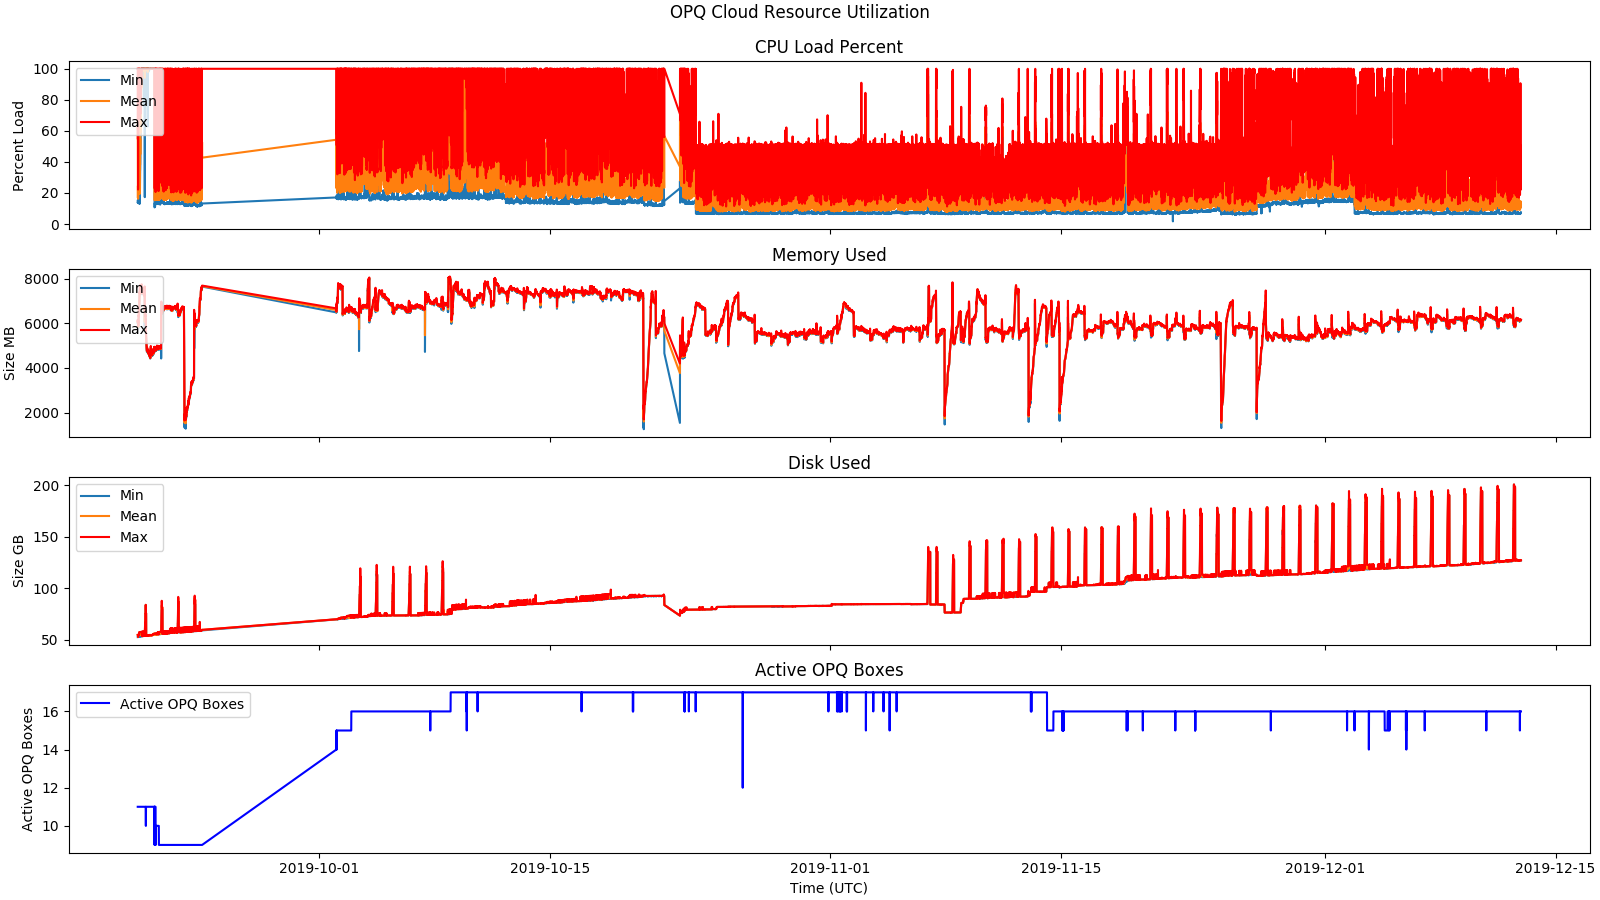
\includegraphics[width=\linewidth]{figures/actual_system_opq.png}
    \caption{System Utilization for OPQ}
    \label{fig:actual_system_opq}
\end{figure}

You'll note gaps in the data in early and mid October. These were caused by a mix-up in deployed branches where one of the branches did not have collection of system statistics enabled.

The top panel shows the minimum, mean, and maximum CPU load. Each triplet of min, mean, and max values are aggregated over 30 sample points. So even though the CPU hits 100\% utilization quite often, the mean of the CPU utilization is much lower, rarely rising over 40\%. A slight decrease (~5\%) in CPU load can be observed when the second virtual CPU was added to the system.

I expect that we could double the amount of deployed sensors to 30 and still see mean CPU utilization less than 80\%. Beyond that would require either more powerful hardware or distributing OPQ services over multiple servers.

The second panel shows memory utilization. OPQ utilizes on average close to 75\% of the available memory. I dug a little bit deeper into how the memory was being utilized and found a perhaps unsurprising result. Table~\ref{table:mem_utilization} shows the breakdown of largest memory utilization on our system.

\begin{table}[H]
    \centering
    \caption{OPQ Large Memory Utilization}
    \begin{tabularx}{\textwidth}{Xl}
        \toprule
        \textbf{Process} & \textbf{\% Memory} \\
        \midrule
        MongoDB & 51 \\
        OPQ Mauka & 8 \\
        OPQ View & .8 \\
        OPQ Makai & .3 \\
        Docker & .3 \\
        OPQ Box Updater & .1 \\
        JournalD & .1 \\
        \bottomrule
    \end{tabularx}
    \label{table:mem_utilization}
\end{table}

MongoDB uses over half of our available memory! This should be somewhat unsurprising because MongoDB aggressively caches data in-memory for efficient queries. No matter how much memory is on our system, MongoDB will use a large chunk of it. All of the OPQ Mauka processes combined only add up to about 8\% memory utilization with 15 sensors. I estimate that on current hardware, Mauka could handle up to about 100 sensors and still remain within 80\% memory utilization (of course this would have an adverse affect on MongoDB caching).

The third panel shows disk usage over time. As of about two and a half months into data collection, the server is storing about 130 GB worth of data. One interesting feature of this plot are the periodic spikes. The periodic spikes are caused by daily database backups. Every day, a backup of the database is performed, compressed, and written to disk. It is then uploaded to cloud storage and on successful upload, deleted locally. There is a large gap of these spike near the end of October and beginning of November. This gap is the result of a Docker bug that inhibited our system from performing daily backups. I changed the backup routine to use a local MongoDB client rather than one provided by Docker and the daily backups resumed.

The bottom panel shows the number of active OPQ Boxes sending over time. There does not appear to be a large correlation between the number of boxes sending and system resource utilization. This is likely due to the fact that the standard deviation between the number of active OPQ Boxes is quite small ($\sigma=1.63$).

\subsection{DSN System Requirements: Lokahi}\label{subsec:dsn-system-requirements:-lokahi}

\subsubsection{DSN System Requirements Lokahi: IML}

\subsubsection{DSN System Requirements Lokahi: AML}

\subsubsection{DSN System Requirements Lokahi: DL}

\subsubsection{DSN System Requirements Lokahi: IL}

\subsubsection{DSN System Requirements Lokahi: PL}

\subsection{Ground Truth Analysis}

\subsection{Ground Truth Analysis: OPQ}

The UHM Office of Energy Management provided out team with access to data collected by high quality power meters installed at the mains of selected campus buildings. This data set provides the basis of the ground truth data that I collected.

Ground truth data was scraped from an UHM internal server over the duration of the OPQ deployment. I collected ground truth data containing 15 features for each of the ground truth meters that are co-located with an OPQ Box. The ground truth data is mostly complete, however, there are a few missing features for some meters.

The provided ground truth data is similar to OPQ Trends in that it provides rolled up summary statistics for features over a window of 60 seconds. The included statistics include the actual, minimum, maximum, average, and standard deviation of the features measured.

I collected the following available features for ground truth: ``Frequency", ``Average Voltage THD", ``VAB", ``VAN", ``VBC", ``VBN", ``VCA", ``VCN", ``Voltage CN THD", ``Voltage AN THD", ``Voltage BN THD", and ``Voltage CN THD".

The Frequency and THD measurements are in units that similar to what OPQ collects (Frequency @ 60Hz and \% THD), but the Voltage values are in RMS at 420V and 240V where OPQ collects RMS at 120V. This means that the Voltage values can not be compared directly and that we either need to scale the Voltage values or use straight thresholds for determining Events and Incidents. Further, the ground truth values for Voltage are provided for each of the three Voltage phases whereas OPQ Boxes compute RMS Voltage from a combination of three phases. This needs to be considered before comparing ground truth Voltage to OPQ Voltage measurements.

To complicate things, we do not have a UHM meter co-located with every OPQ Box and several of our Boxes are co-located with multiple UHM meters making the determination of which combination of Box and Meter to compare arduous.

Finally, it should be noted that because of OPQ's TTL, Measurements are only stored for a day and Trends are only stored for two weeks.

\subsubsection{Frequency Analysis}

\begin{figure}
    \begin{tabular}{ccc}
        \subfloat[caption]{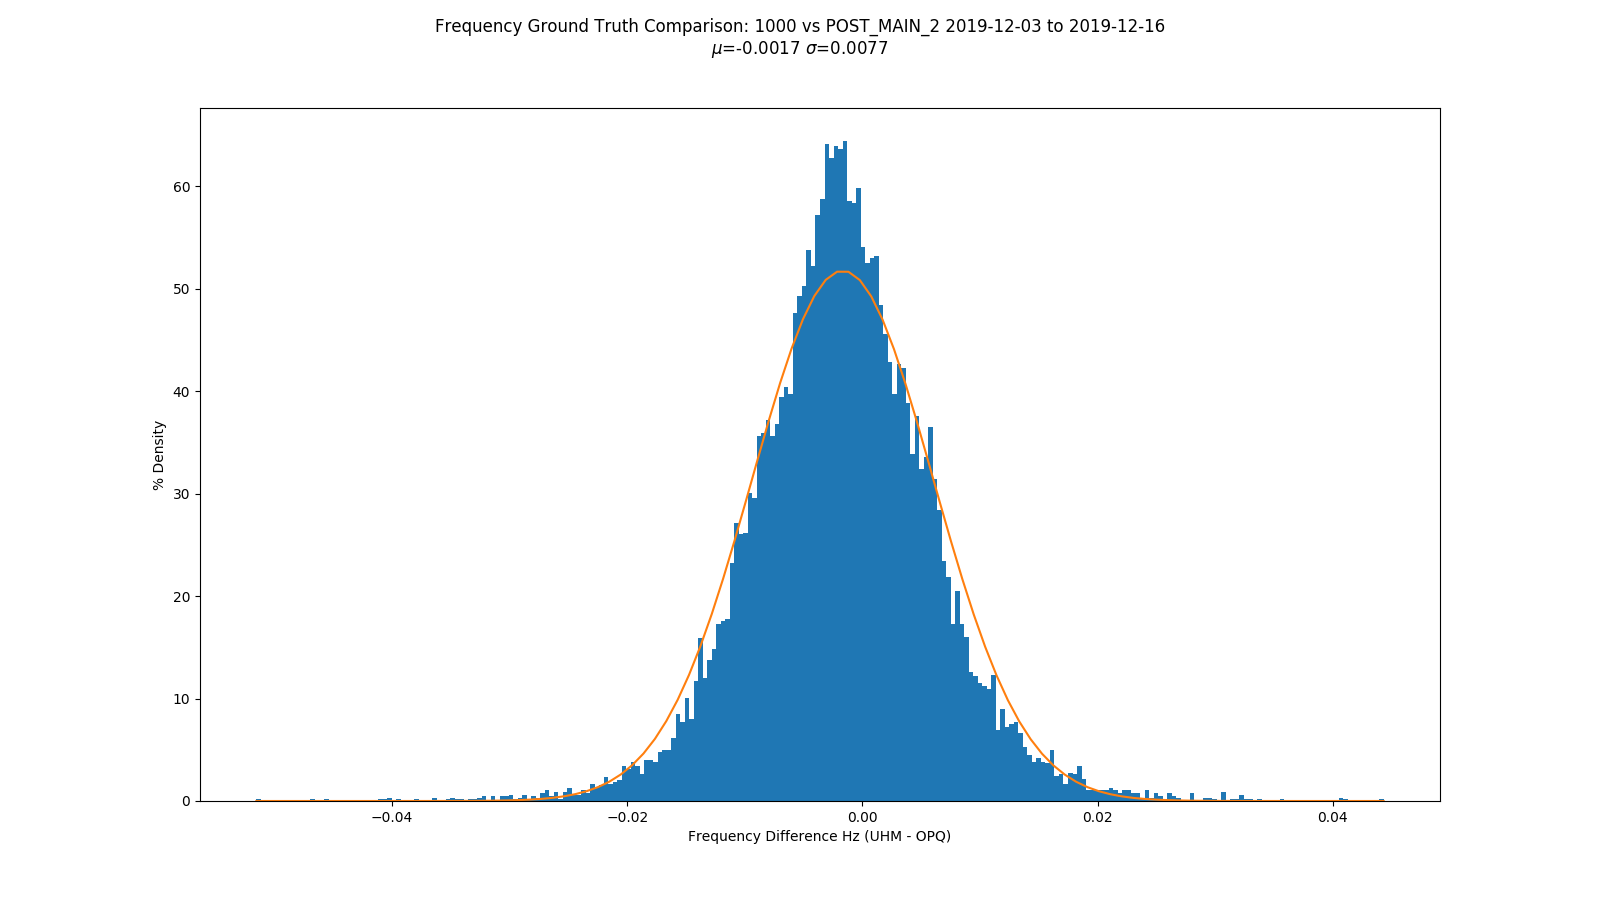
\includegraphics[width = .3\linewidth]{figures/f_hist_1000_POST_MAIN_2.png}} &
        \subfloat[caption]{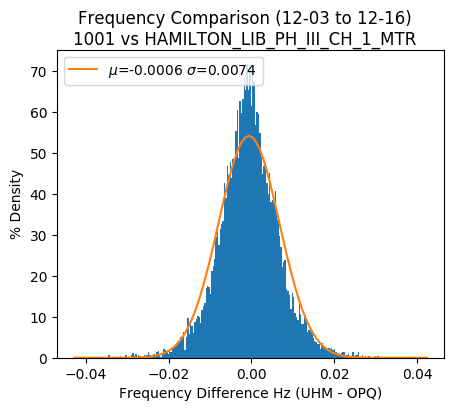
\includegraphics[width = .3\linewidth]{figures/f_hist_1001_HAMILTON_LIB_PH_III_CH_1_MTR.png}} &
        \subfloat[caption]{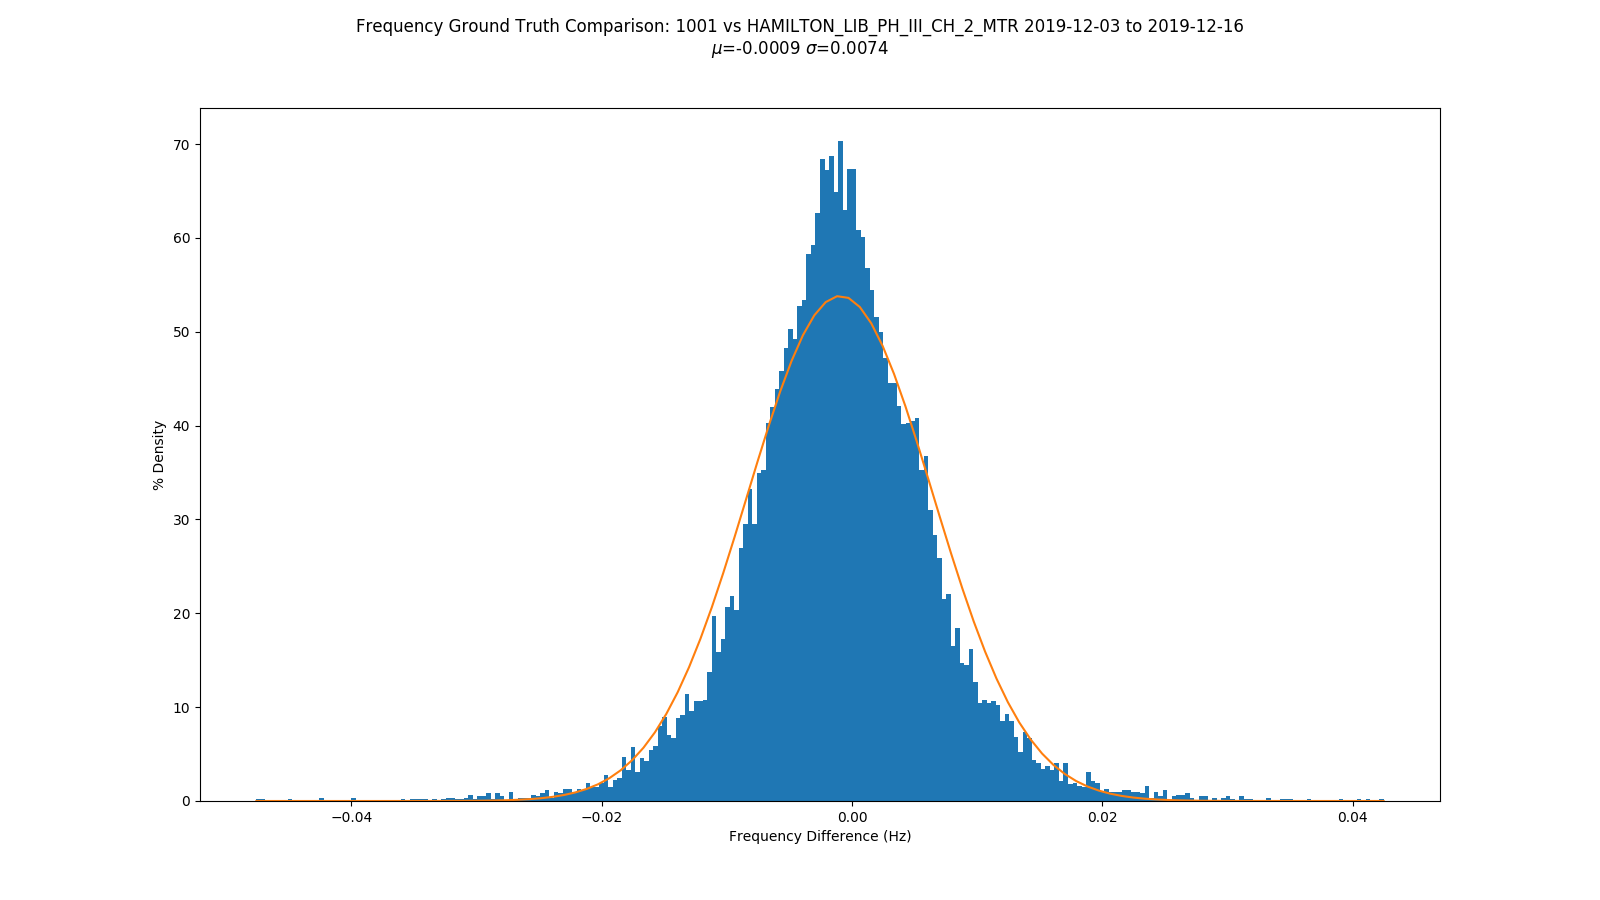
\includegraphics[width = .3\linewidth]{figures/f_hist_1001_HAMILTON_LIB_PH_III_CH_2_MTR.png}}  \\
        \subfloat[caption]{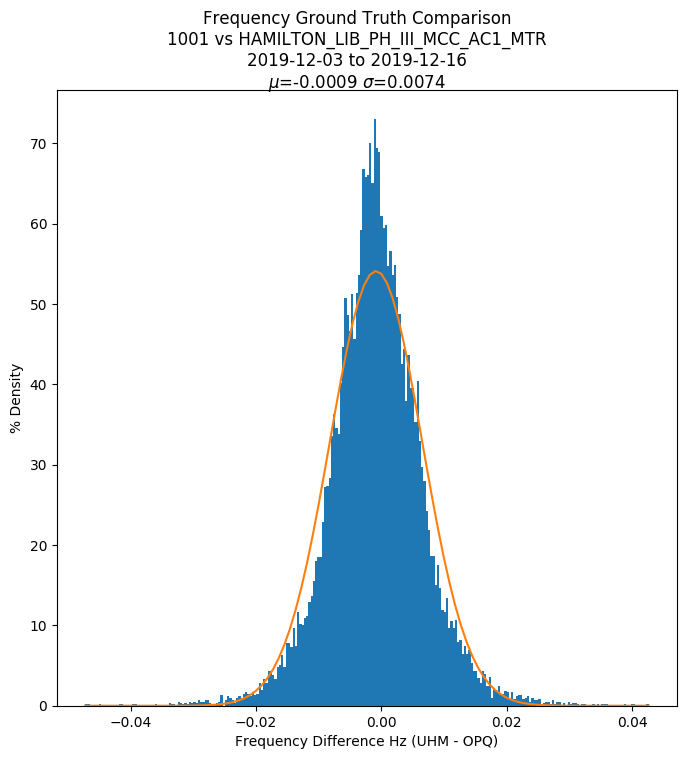
\includegraphics[width = .3\linewidth]{figures/f_hist_1001_HAMILTON_LIB_PH_III_MCC_AC1_MTR.png}} &
        \subfloat[caption]{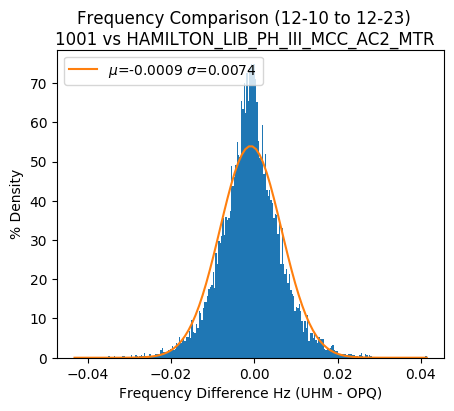
\includegraphics[width = .3\linewidth]{figures/f_hist_1001_HAMILTON_LIB_PH_III_MCC_AC2_MTR.png}} &
        \subfloat[caption]{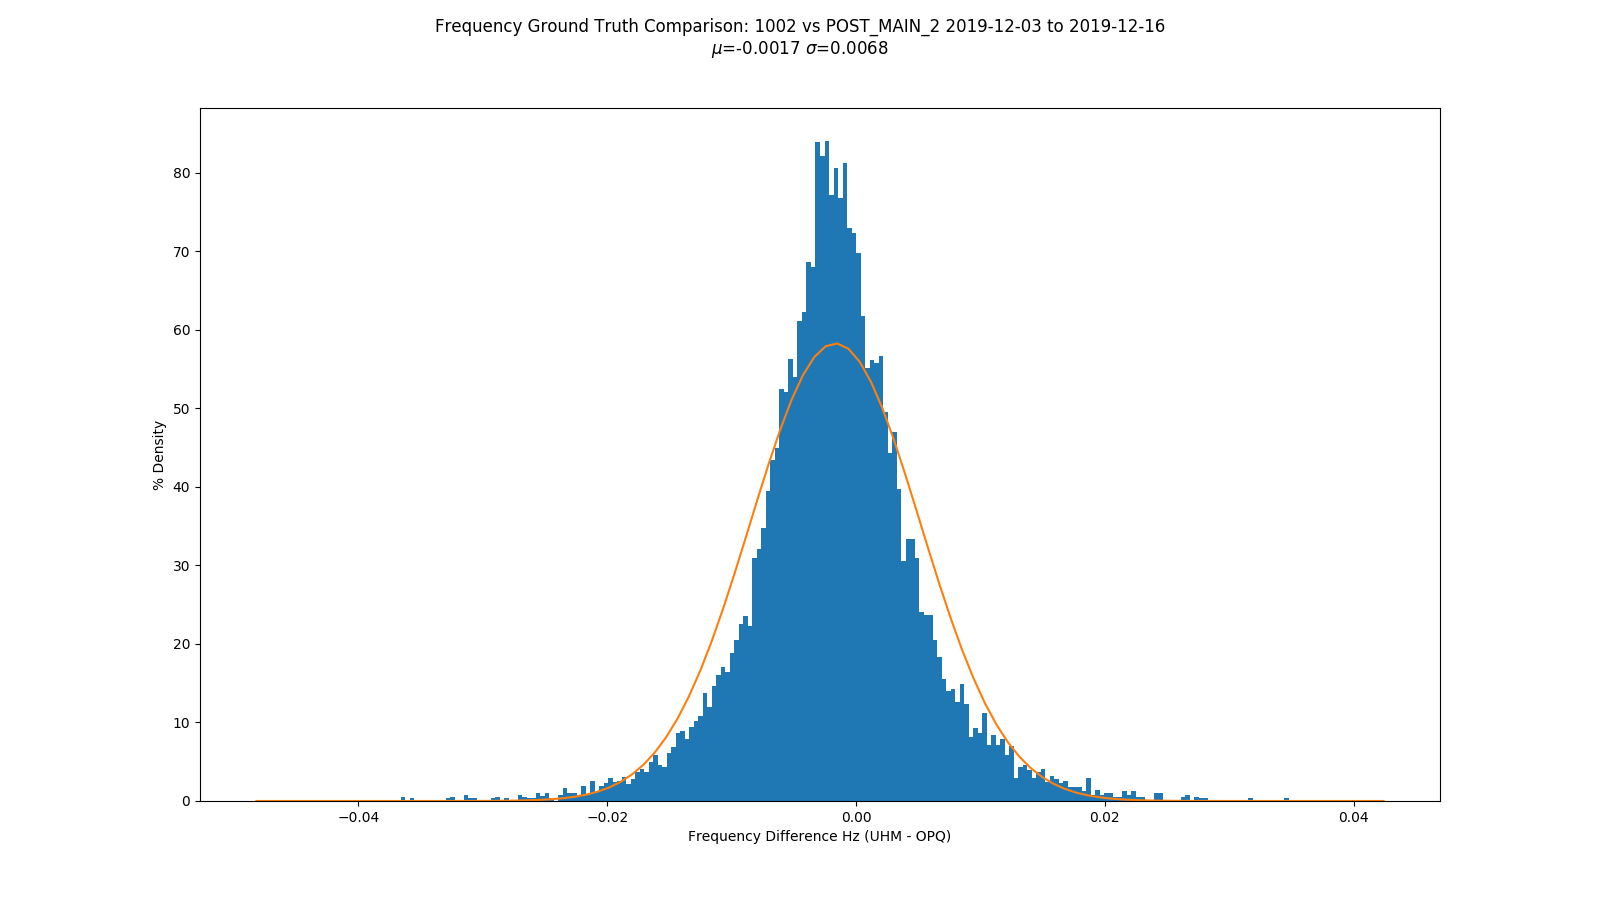
\includegraphics[width = .3\linewidth]{figures/f_hist_1002_POST_MAIN_2.png}} \\
    \end{tabular}
    \caption{4 x 4}
\end{figure}

%Figure~\ref{fig:f_hist_1000_POST_MAIN_2}
%
%\begin{figure}[H]
%    \centering
%    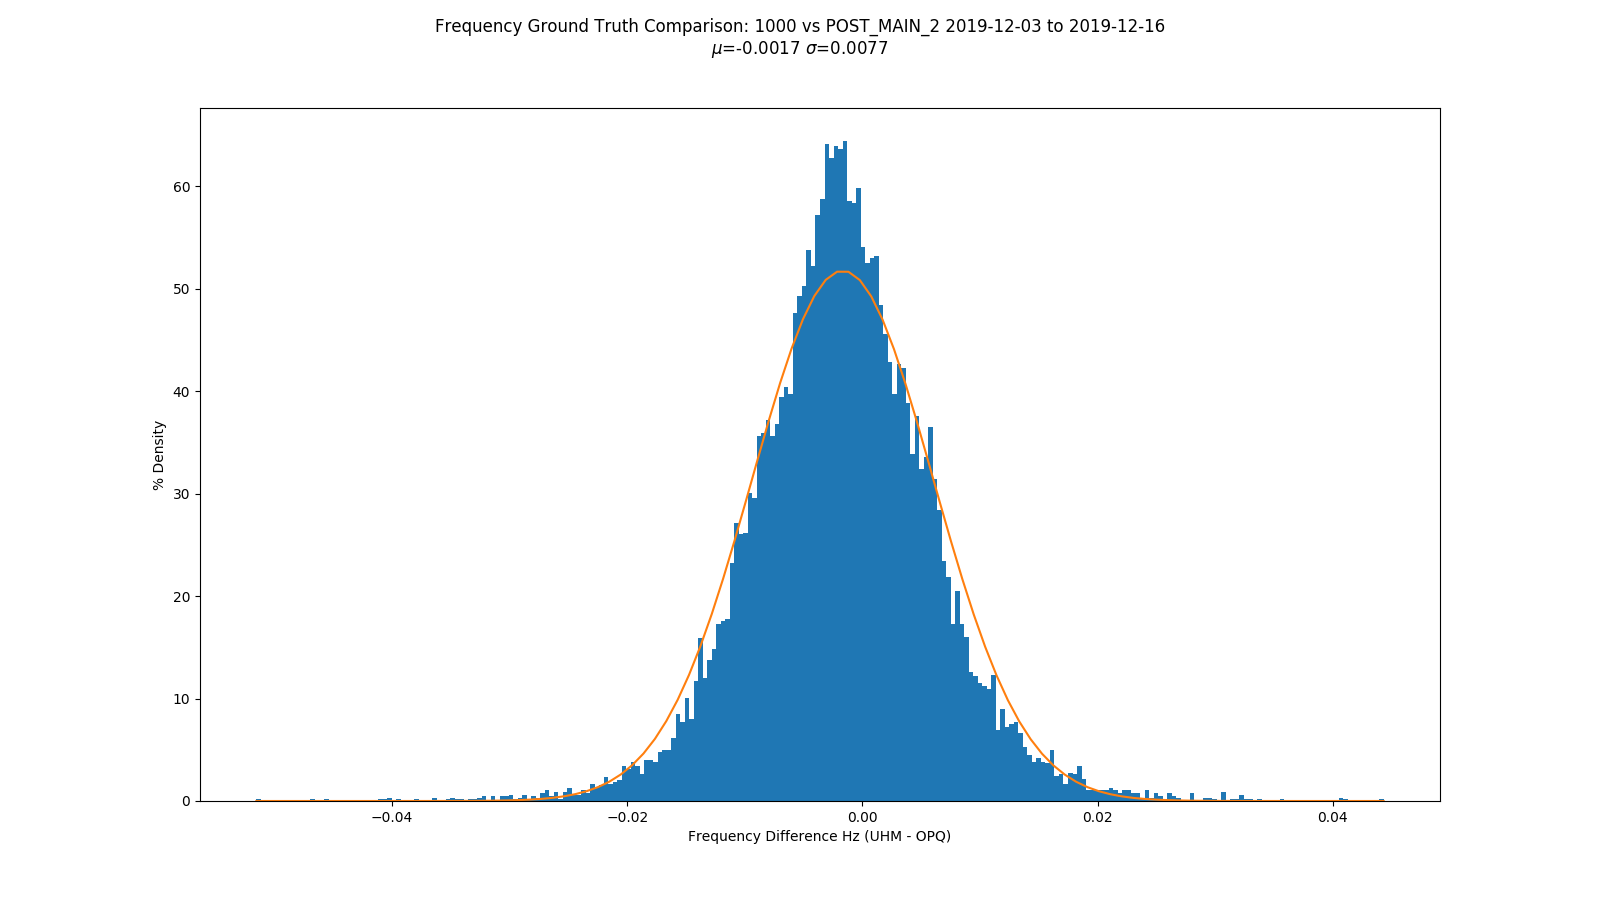
\includegraphics[width=\linewidth]{figures/f_hist_1000_POST_MAIN_2.png}
%    \caption{}
%    \label{fig:f_hist_1000_POST_MAIN_2}
%\end{figure}
%
%Figure~\ref{fig:f_hist_1001_HAMILTON_LIB_PH_III_CH_1_MTR}
%
%\begin{figure}[H]
%    \centering
%    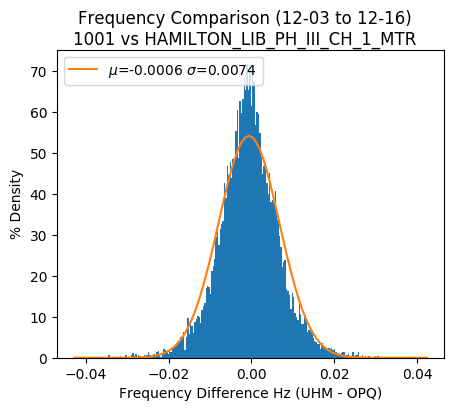
\includegraphics[width=\linewidth]{figures/f_hist_1001_HAMILTON_LIB_PH_III_CH_1_MTR.png}
%    \caption{}
%    \label{fig:f_hist_1001_HAMILTON_LIB_PH_III_CH_1_MTR}
%\end{figure}
%
%Figure~\ref{fig:f_hist_1001_HAMILTON_LIB_PH_III_CH_2_MTR}
%
%\begin{figure}[H]
%    \centering
%    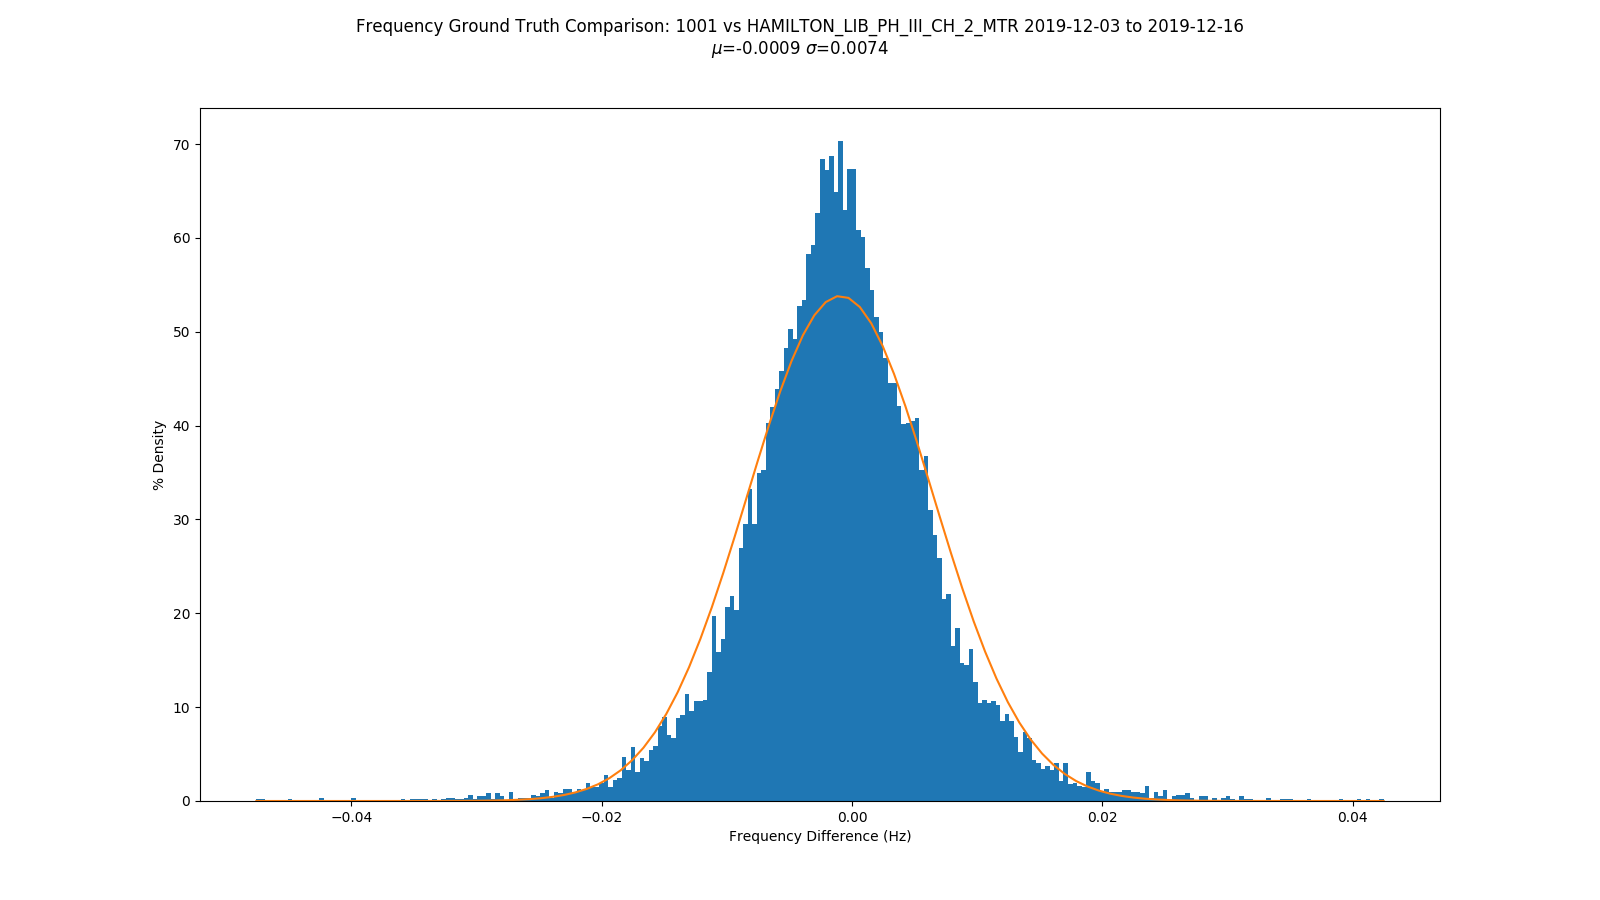
\includegraphics[width=\linewidth]{figures/f_hist_1001_HAMILTON_LIB_PH_III_CH_2_MTR.png}
%    \caption{}
%    \label{fig:f_hist_1001_HAMILTON_LIB_PH_III_CH_2_MTR}
%\end{figure}

Figure~\ref{fig:f_hist_1001_HAMILTON_LIB_PH_III_CH_3_MTR}

\begin{figure}[H]
    \centering
    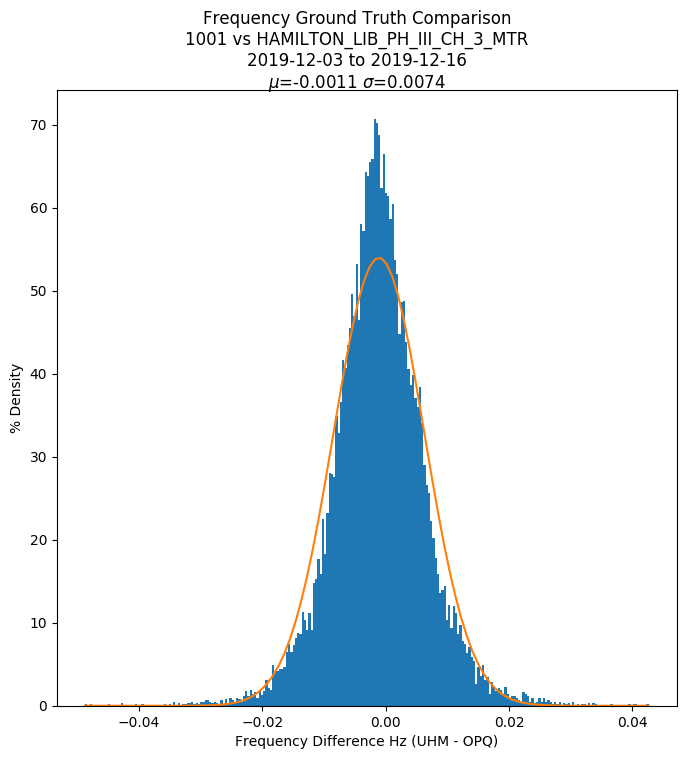
\includegraphics[width=\linewidth]{figures/f_hist_1001_HAMILTON_LIB_PH_III_CH_3_MTR.png}
    \caption{}
    \label{fig:f_hist_1001_HAMILTON_LIB_PH_III_CH_3_MTR}
\end{figure}

Figure~\ref{fig:f_hist_1001_HAMILTON_LIB_PH_III_MCC_AC1_MTR}

\begin{figure}[H]
    \centering
    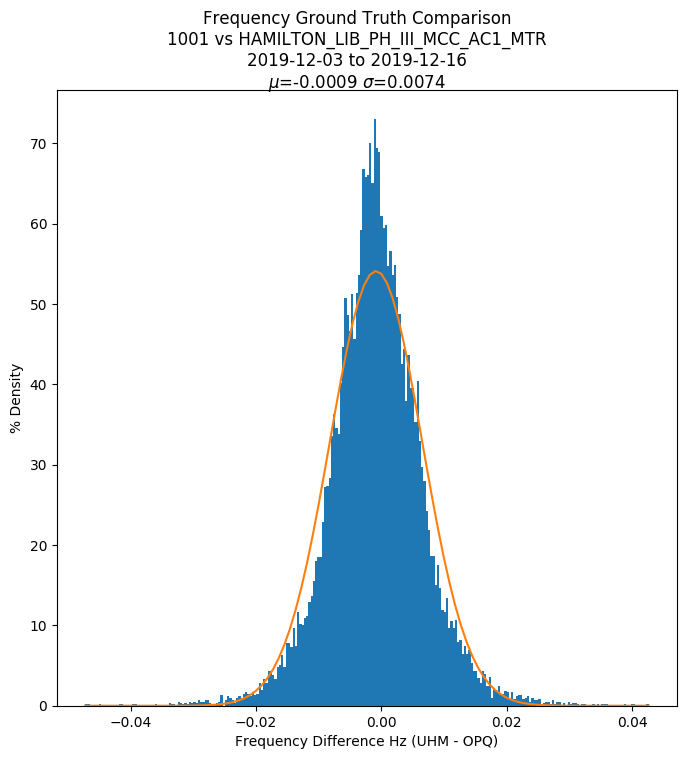
\includegraphics[width=\linewidth]{figures/f_hist_1001_HAMILTON_LIB_PH_III_MCC_AC1_MTR.png}
    \caption{}
    \label{fig:f_hist_1001_HAMILTON_LIB_PH_III_MCC_AC1_MTR}
\end{figure}

Figure~\ref{fig:f_hist_1001_HAMILTON_LIB_PH_III_MCC_AC2_MTR}

\begin{figure}[H]
    \centering
    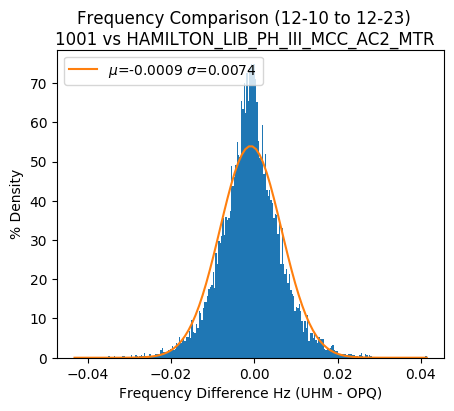
\includegraphics[width=\linewidth]{figures/f_hist_1001_HAMILTON_LIB_PH_III_MCC_AC2_MTR.png}
    \caption{}
    \label{fig:f_hist_1001_HAMILTON_LIB_PH_III_MCC_AC2_MTR}
\end{figure}

Figure~\ref{fig:f_hist_1002_POST_MAIN_2}

\begin{figure}[H]
    \centering
    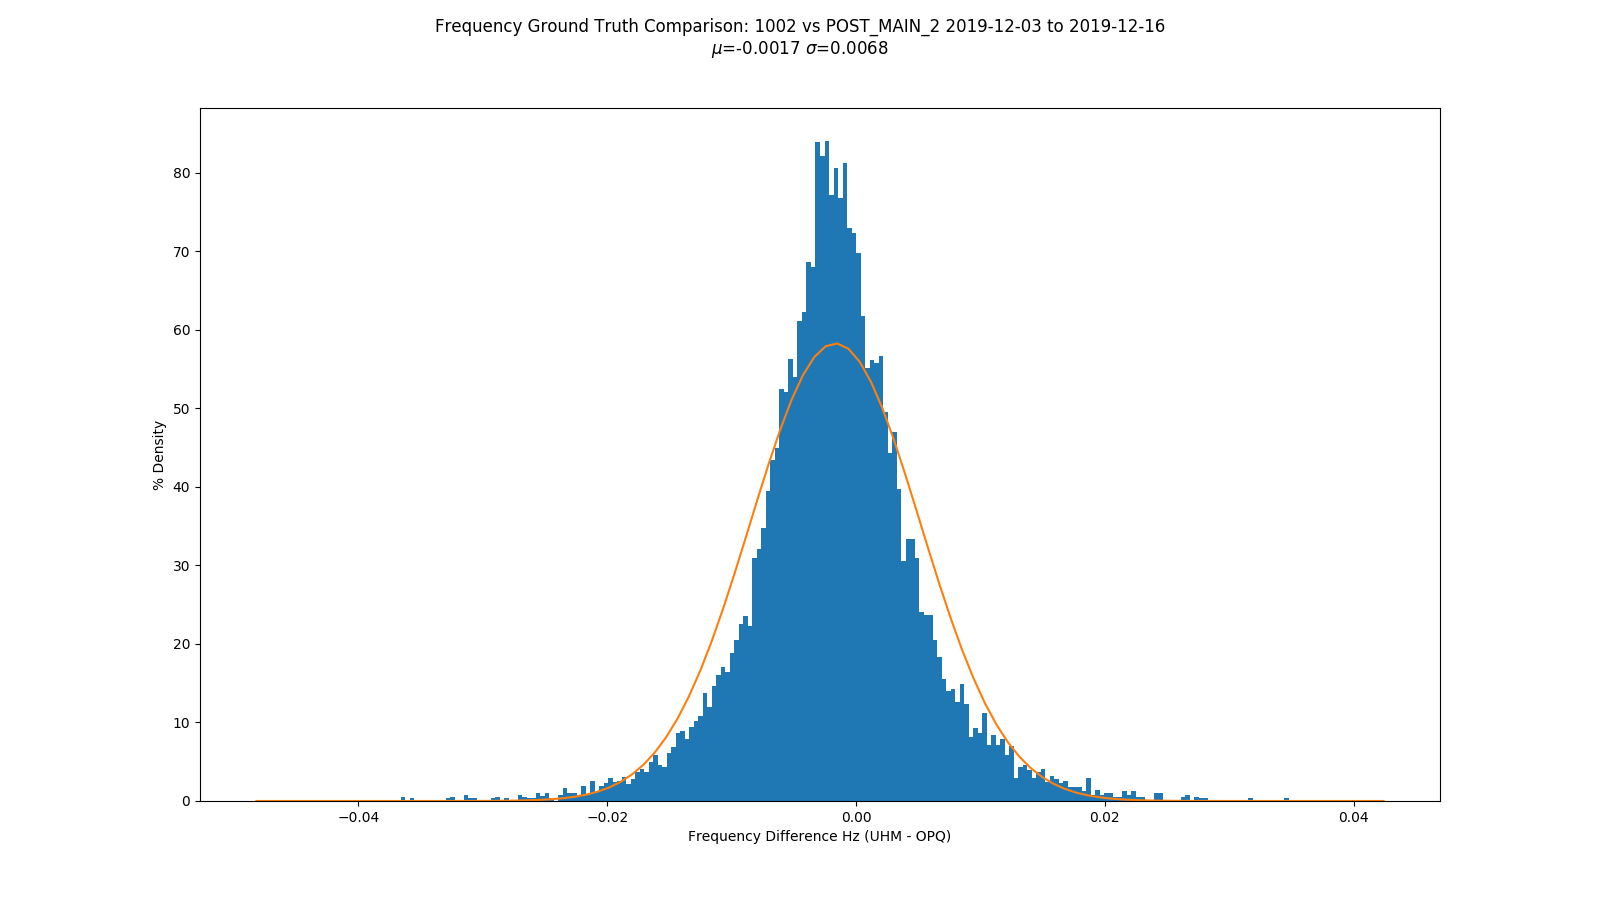
\includegraphics[width=\linewidth]{figures/f_hist_1002_POST_MAIN_2.png}
    \caption{}
    \label{fig:f_hist_1002_POST_MAIN_2}
\end{figure}

Figure~\ref{fig:f_hist_1003_KELLER_HALL_MAIN_MTR}

\begin{figure}[H]
    \centering
    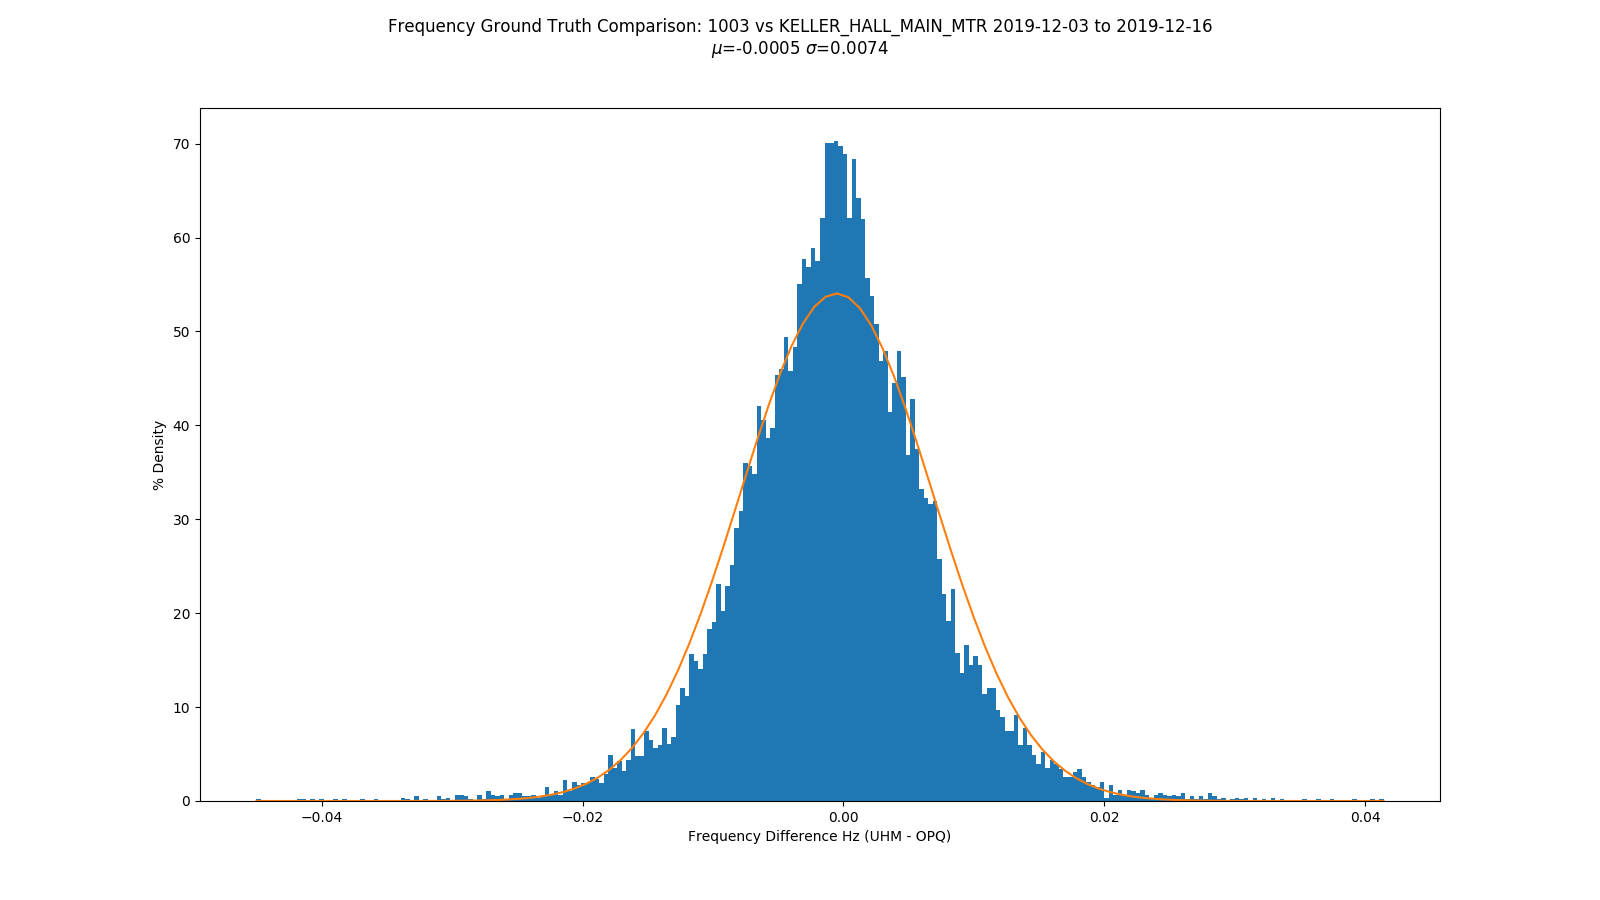
\includegraphics[width=\linewidth]{figures/f_hist_1003_KELLER_HALL_MAIN_MTR.png}
    \caption{}
    \label{fig:f_hist_1003_KELLER_HALL_MAIN_MTR}
\end{figure}

Figure~\ref{fig:f_hist_1021_MARINE_SCIENCE_MAIN_A_MTR}

\begin{figure}[H]
    \centering
    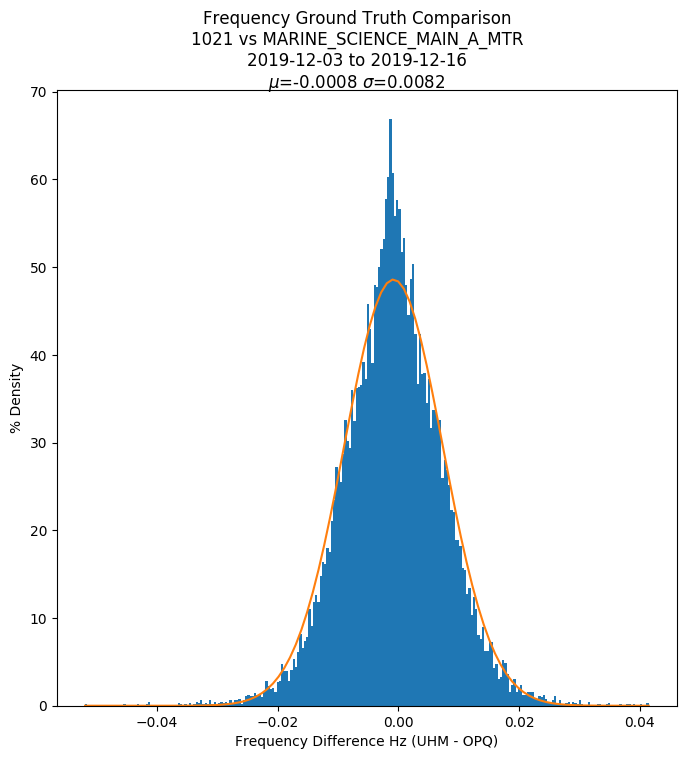
\includegraphics[width=\linewidth]{figures/f_hist_1021_MARINE_SCIENCE_MAIN_A_MTR.png}
    \caption{}
    \label{fig:f_hist_1021_MARINE_SCIENCE_MAIN_A_MTR}
\end{figure}

Figure~\ref{fig:f_hist_1021_MARINE_SCIENCE_MAIN_B_MTR}

\begin{figure}[H]
    \centering
    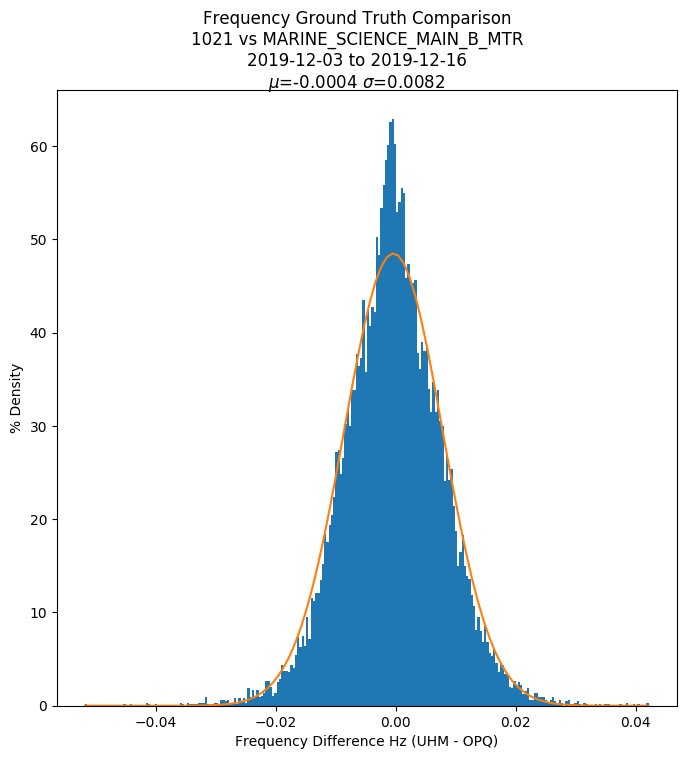
\includegraphics[width=\linewidth]{figures/f_hist_1021_MARINE_SCIENCE_MAIN_B_MTR.png}
    \caption{}
    \label{fig:f_hist_1021_MARINE_SCIENCE_MAIN_B_MTR}
\end{figure}

Figure~\ref{fig:f_hist_1022_AG_ENGINEERING_MAIN_MTR}

\begin{figure}[H]
    \centering
    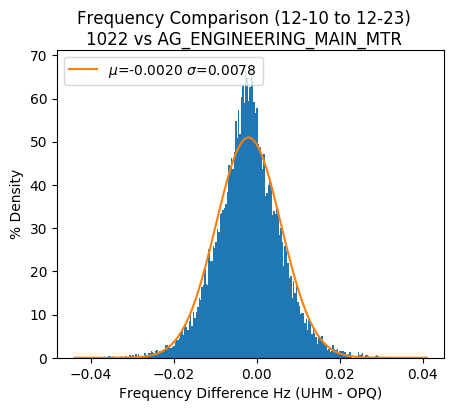
\includegraphics[width=\linewidth]{figures/f_hist_1022_AG_ENGINEERING_MAIN_MTR.png}
    \caption{}
    \label{fig:f_hist_1022_AG_ENGINEERING_MAIN_MTR}
\end{figure}

Figure~\ref{fig:f_hist_1022_AG_ENGINEERING_MCC_MTR}

\begin{figure}[H]
    \centering
    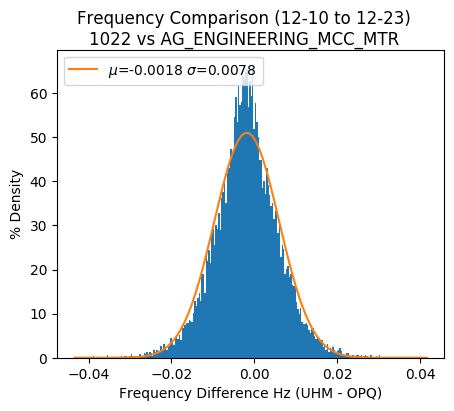
\includegraphics[width=\linewidth]{figures/f_hist_1022_AG_ENGINEERING_MCC_MTR.png}
    \caption{}
    \label{fig:f_hist_1022_AG_ENGINEERING_MCC_MTR}
\end{figure}

Figure~\ref{fig:f_hist_1023_LAW_LIB_MAIN_MTR}

\begin{figure}[H]
    \centering
    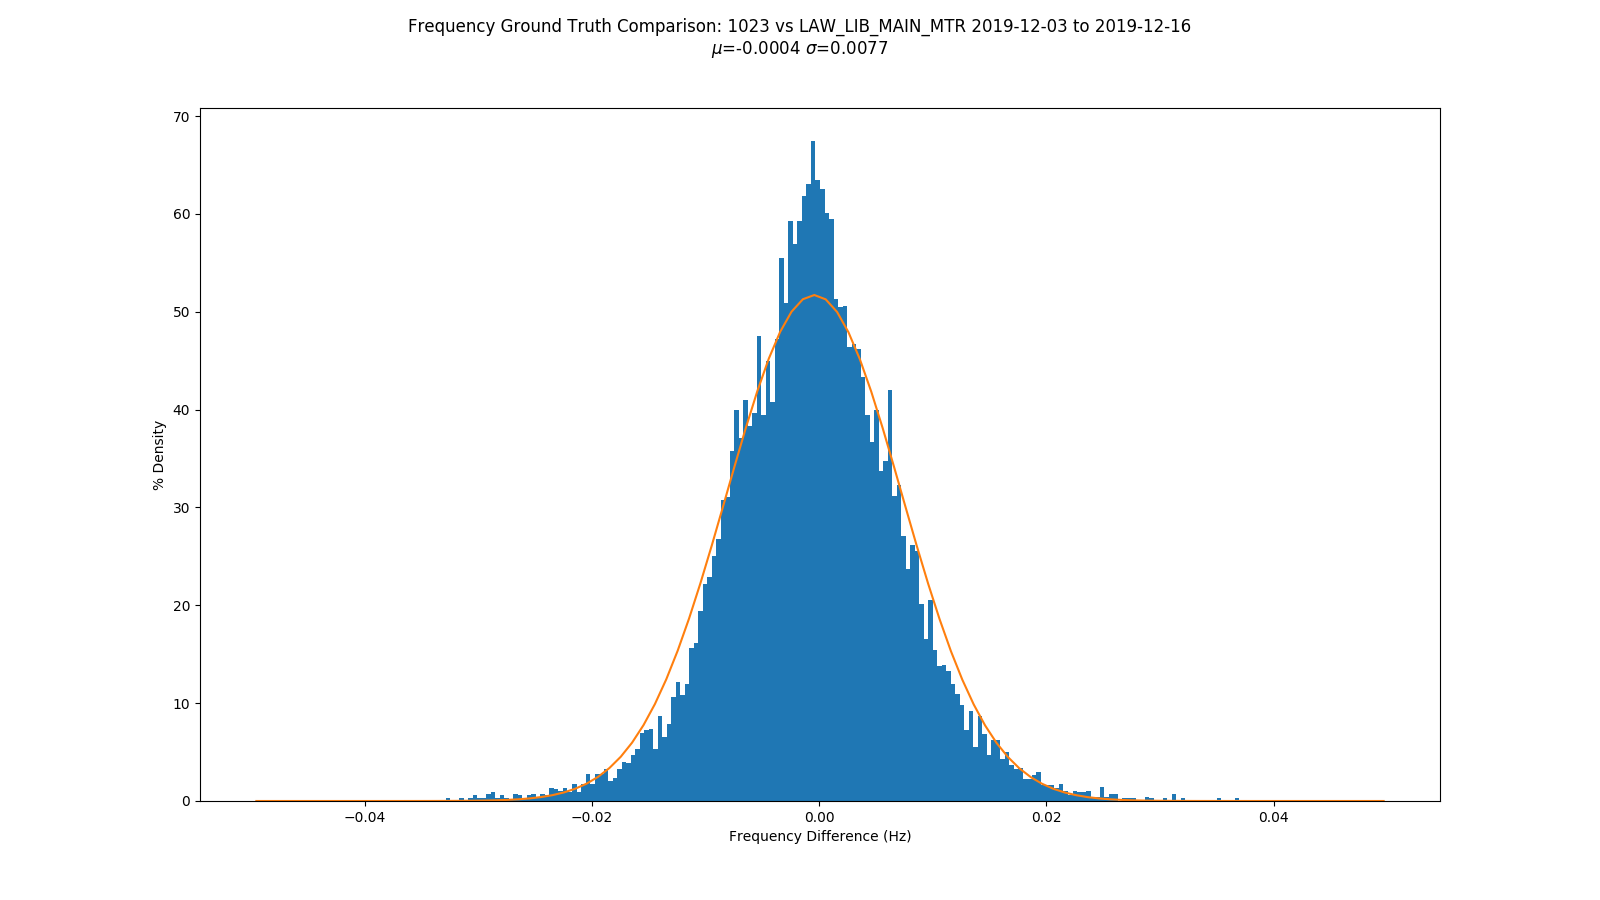
\includegraphics[width=\linewidth]{figures/f_hist_1023_LAW_LIB_MAIN_MTR.png}
    \caption{}
    \label{fig:f_hist_1023_LAW_LIB_MAIN_MTR}
\end{figure}

Figure~\ref{fig:f_hist_1025_KENNEDY_THEATRE_MAIN_MTR}

\begin{figure}[H]
    \centering
    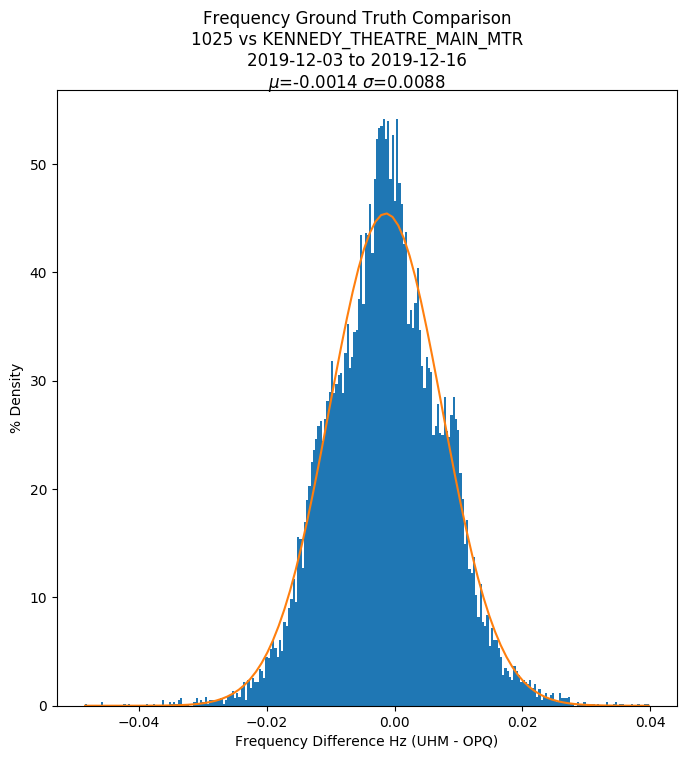
\includegraphics[width=\linewidth]{figures/f_hist_1025_KENNEDY_THEATRE_MAIN_MTR.png}
    \caption{}
    \label{fig:f_hist_1025_KENNEDY_THEATRE_MAIN_MTR}
\end{figure}

\chapter{Conclusions}\label{ch:conclusion}

This dissertation presented the Laha abstract distributed sensor network framework.

Chapter~\ref{ch:introduction} introduced the Laha framework (Section~\ref{sec:laha:-an-abstract-framework-for-adaptively-optimizing-dsns}) and the main problems that the Laha Framework aims to solve, namely the conversion of primitive sensor data into actionable insights (Section~\ref{sec:converting-sensor-data-into-actionable-insights}) and the management of Big Data in relation to DSNs (Section~\ref{sec:big-data-management-in-dsns}). Traditional approaches to DSN optimization were briefly examined (Section~\ref{sec:traditional-approaches-to-dsn-optimization}). This chapter also provided the major claims of the Laha framework (Section~\ref{sec:anticipated-contributions-of-laha}) as well as the major contributions to the field of DSNs (Section~\ref{subsec:anticipated-contributions}).

Chapter~\ref{ch:related-work} examined related work with an emphasis on Big Data and distributed sensor networks (Section~\ref{sec:big-data-and-distributed-sensor-networks}), DSN Big Data management (Section~\ref{sec:distributed-sensor-networks-and-big-data-management}), predictive analytics and forecasting for DSNs (Section~\ref{sec:distributed-sensor-networks-and-predictive-analytics-and-forecasting}), topology and localization (Section~\ref{sec:determining-topology-and-localization}), and triggering optimizations (Section~\ref{sec:optimizations-for-triggering}).

Chapter~\ref{ch:system-design} provided the design details of the Laha framework as well as the design details for the Lokahi and OPQ Laha-compatible reference networks. This chapter included the design of the Laha hierarchy for DSN Big Data Management (Section~\ref{sec:big-data-management}), the design of Phenomena (Section~\ref{sec:phenomena}), design of Laha Actors (Section~\ref{sec:laha-actors:-acting-on-the-laha-data-model}), design of the OPQ reference network (Section~\ref{sec:opq:-a-laha-compliant-power-quality-dsn}), and the design of the Lokahi reference network (Section~\ref{sec:lokahi:-a-laha-compliant-infrasound-dsn}).

Chapter~\ref{ch:evaluation} provided evaluation techniques for determining if the Laha framework is able to meet the goals set in the Introduction chapter. In particular, this chapter examined deployment plans for the OPQ and Lokahi networks (Section~\ref{sec:deploy-laha-reference-implementations-on-test-sites}), data validation strategies (Section~\ref{sec:validate-data-collected-by-laha-deployment}), the evaluation of determining if Laha meets the goals stated in the Introduction chapter (Section~\ref{sec:use-laha-deployments-to-evaluate-the-main-goals-of-the-framework}), and a set of tertiary goals for evaluation (Section~\ref{sec:evaluation-of-tertiary-goals}).

Chapter~\ref{ch:results} provided evidence and results from the Lokahi and OPQ networks that were used to give credence to the goals and contributions outlined in the Introduction chapter. Results were provided for data validation (Section~\ref{sec:ground-truth-analysis}), the generality of the Laha framework (Section~\ref{sec:results-of-generality-of-this-framework}), the ability to convert primitive sensor data into actionable insights (through the Laha level hierarchy and Phenomena (Section~\ref{sec:results-of-converting-primitie-data-into-actional-insights})), tiered Big Data management (Section~\ref{sec:dsn-system-requirements}), and results for the provided tertiary goals (Section~\ref{sec:results-of-tertiary-goals}).

The results showed that Laha is a general framework that can be applied to multiple DSN domains. I showed in the results section that both the OPQ and Lokahi networks were able to meet the stated goals of those networks. In particular, the OPQ network was able to identify distributed PQ signals consisting of transient, voltage, and frequency deviations while the Lokahi network was able to identify infrasonic signals of interest from multiple sources including storms, explosions, and atmospheric disturbances. I showed that the Laha framework is able to convert primitive data into actionable insights through its level hierarchy and also through Phenomena which provide groupings of Incidents and predictive analytic capabilities. I showed that the Laha level hierarchy in conjunction with TTL provides enhanced data management in the form of reducing sensor noise and network resource consumption requirements. Results for TTL of data showed an overall data reduction of close to 96\%. I showed that Phenomena are able to optimize lower levels of the Laha hierarchy which increase its ability to detect sub-threshold Events, detect periodic signals of interest, predict future signals of interest, and reduce data storage requirements which form the basis of Laha's tertiary goals.

\section{Future Directions}\label{sec:future-directions}

The longer I've worked with these networks, the more I've realized that they could be expanded in a multitude of ways.

\subsection{Machine Learning}\label{subsec:machine-learning}
I think the lowest hanging fruit for Laha is to implement a machine learning layer. I believe machine learning could be used for triggering, detection, and classification of signals of interest. This is an active area of research within the Lokahi network as we are currently planning to augment our architecture with machine learning. The goals for machine learning within Lokahi are to implement robust detection algorithms using a training set of labeled data collected at our lab and at various national laboratories.

I also believe machine learning could be useful at the Phenomena level, providing models for predicting Events and Incidents and identifying groupings of data. It could be useful to augment Annotation Phenomena with the ability to automatically create new Annotations from past data.

\subsection{Modifying Windows and Thresholds}\label{subsec:modifying-windows-and-thresholds}
To improve the process of creating Events and Incidents, I believe it would be useful to experiment with changing window sizes used to compute low level metrics such as Frequency, THD, and Voltage. As shown in the ground truth analysis, the current implementation uses cycle sized windows for computing THD and frequency, but has a cost of added noise. These window sizes could be modified to find an optimum length that minimizes noise, but still accurately reflects the data. By minimizing noise, the system is able to store less data while maximizing system resource allocation for the detection and analysis of signals of interest. As networks scale, this problem becomes more pronounced and noise reduction becomes even more relevant. This is especially true for resource constrained networks which may not have the resources required for storing and filtering data with a low signal-to-noise ratio.

\subsection{More Simulations}\label{subsec:more-simulations}
Although I created a simulation to simulate Laha itself, I believe it would be useful to simulate the power grid as well. Multiple commercial options exist that provide grid simulations. It could be useful to create a copy of the UHM micro-grid in simulation to help fill in some of the missing puzzle pieces about sensor topology and how signals travel through the UHM micro-grid. This would also afford us the opportunity to simulate PQ signals at will instead of waiting for them to arrive. Simulations could allow researchers to more accurately model the sensing field topology. Simulations could also be used to determine optimum sensor placement when sensor availability is low, increasing the chances of identifying target signals of interest. Simulations could also allow us to model the Laha hierarchy in situations where the ground truth is not known or the sensing field topology is unknown.

\subsection{Altering the Laha Level Hierarchy}\label{subsec:altering-the-laha-level-hierarchy}
I would like to experiment with adding and/or combining levels within the Laha hierarchy as described in the ``Discussion of Laha Levels" section. An additional Sensor Measurement Level could be implemented to differentiate between data stored on sensors and data that is stored ``in the cloud". Data stored in the cloud would utilize the same IML level that currently exists, but instead of copying IML data into higher levels, higher levels would simply point to the IML data. An experiment could be constructed that measures the amount of data stored on sensors at any one time versus the amount of data stored in the cloud with respect to raw sensor samples. This experiment would also examine data savings provided by pointing to IML data instead of copying IML data into higher Laha levels.

I believe that Laha is a perfect test bed for data fusion. I would like to integrate multiple data streams into the DSNs to find correlations in the data providing more context for the signals that we observe. For instance, solar production and other environmental data would provide useful data streams for the OPQ network to compare signals against. These new data streams would be provided in new level called the Data Fusion Level (DFL). Specifically, an experiment comparing solar production to PQ utilizing this new level could provide interesting insights into how distributed renewable energy sources directly affect power quality on the grid. With a high availability of solar energy potential, Hawaii makes a perfect test bed for such an experiment. Other data streams that could be fed into this level include cloud coverage and radar data, precipitation data, and general weather data.

\subsection{Enhanced Metric Collection}\label{subsec:enhanced-metric-collection}
I believe Laha could do a better job at collecting metrics about system performance. It would be good to know exactly when data is garbage collected. It would also be useful to collect more memory and system utilization metrics per plugin to determine the performance overhead of individual pieces of analysis.

Future deployments could investigate utilizing more detailed ground truth metrics. The ground truth metrics utilized by OPQ only provided high level trends for voltage, frequency, and THD. It could be useful to have ground truth metrics that include some sort of indication of anomalous PQ events because the UHM ground truth only provided trend data and Events and Incidents were extracted from the trend data by applying thresholds used in the OPQ network. Ground truth data that has a built-in notion of events could be more accurate than determing where the ground truth data should have observed events.

\subsection{Expanded Sensor Coverage}\label{subsec:expanded-sensor-coverage}
Finally, I would like to develop and deploy more sensors for OPQ outside of the UHM micro-grid. It would be useful to discover the interactions in PQ between multiple grids, island wide, and between islands. By having expanded sensor coverage, I believe OPQ could be utilized for solving larger scale problems. For example, an island wide deployment could be useful for accurately determining how distributed intermittent renewable energy sources affect the power grid as a whole and also how renewable energy sources affect individual communities. A state wide deployment between islands could be useful in determining how different utility providers affect PQ in relation to distributed renewable energy sources. A nation wide deployment of OPQ Boxes could provide details about how multiple connected power grids affect power quality and could provide metrics on how PQ signals travel across the grid on a much larger scale. OPQ Boxes could also be deployed in other countries, specifically developing countries, to better understand where PQ issues arise and provide insights into ways to mitigate these PQ problems. Deployments of OPQ Boxes near sensitive electronics (such as server farms) could be used to monitor PQ and its affects on electronic equipment, potentially alerting users to problems before they occur and providing cost savings in terms of reduced hardware maintenance and turnover.



%%% Switch to appendix mode
\appendix

%%% Bring in any appendices from external file (optional)
\appendix
\section{Static Data}

\subsection{Mauka Default Configuration}
\label{appendix:MaukaConfig}
\begin{verbatim}

{
	// Enables debugging for Mauka plugins
	"mauka.debug": true,

	// List of plugins to debug
	"mauka.debug.plugins": ["MakaiEventPlugin", "StatusPlugin"],

	// Should the event broker be started with Mauka?
	"mauka.startEventBroker": true,

	// Should the pub/sub broker be started with Mauka?
	"mauka.startPubSubBroker": true,

	// Should the plugins be started with Mauka?
	"mauka.startPlugins": true,

	// Makai's event endpoint
	"zmq.event.interface"           : "tcp://localhost:10000",

	// Makai's triggering endpoint
	"zmq.trigger.interface"         : "tcp://localhost:9899",

	// Mauka's pub/sub broker producer endpoint
	"zmq.mauka.broker.pub.interface": "tcp://*:9883",

	// Mauka's pub/sub broker consumer endpoint
	"zmq.mauka.broker.sub.interface": "tcp://*:9882",

	// Mauka's plugin producer endpoint
	"zmq.mauka.plugin.pub.interface": "tcp://localhost:9882",

	// Mauka's plugin consumer endpoint
	"zmq.mauka.plugin.sub.interface": "tcp://localhost:9883",

	// Plugin manager response endpoint
	"zmq.mauka.plugin.management.rep.interface": "tcp://*:12000",

	// Plugin manager request endpoint
	"zmq.mauka.plugin.management.req.interface": "tcp://localhost:12000",

	// MongoDB host
	"mongo.host": "localhost",

	// MongoDB port
	"mongo.port": 27017,

	// MongoDB database
	"mongo.db": "opq",

	// Plugin heartbeat interval in seconds
	"plugins.base.heartbeatIntervalS": 60.0,

	// ITIC segmentation threshold
	"plugins.IticPlugin.segment.threshold.rms": 0.1,

	// FrequencyVariationPlugin reference frequency
	"plugins.FrequencyVariationPlugin.frequency.ref": 60.0,

	// FrequencyVariationPlugin threshold low
	"plugins.FrequencyVariationPlugin.frequency.variation.threshold.low": 0.1,

	// FrequencyVariationPlugin threshold high
	"plugins.FrequencyVariationPlugin.frequency.variation.threshold.high": 0.1,

	// FrequencyVariationPlugin interruption threshold
	"plugins.FrequencyVariationPlugin.frequency.interruption": 58.0,

	// FrequencyVariationPlugin maximum lull in windows
	"plugins.FrequencyVariationPlugin.max.lull.windows": 3,

	// TransietPlugin noise floor
	"plugins.TransientPlugin.noise.floor" : 6.0,

	// TransietPlugin minimum oscillatory cycles
	"plugins.TransientPlugin.oscillatory.min.cycles" : 3,

	// TransietPlugin low frequency max hz
	"plugins.TransientPlugin.oscillatory.low.freq.max.hz" : 5000.0,

	// TransietPlugin medium frequency max hx
	"plugins.TransientPlugin.oscillatory.med.freq.max.hz" : 500000.0,

	// TransietPlugin high frequency max hz
	"plugins.TransientPlugin.oscillatory.high.freq.max.hz" : 5000000.0,

	// TransietPlugin Zero crossing threshold
	"plugins.TransientPlugin.arcing.zero.crossing.threshold" : 10,

	// TransietPlugin Maximum lull in milliseconds
	"plugins.TransientPlugin.max.lull.ms" : 4.0,

	// TransietPlugin periodic notching standard deviation
	"plugins.TransientPlugin.max.periodic.notching.std.dev" : 2.0,

	// TransietPlugin periodicity threshold
	"plugins.TransientPlugin.auto.corr.thresh.periodicity" : 0.4,

	// MakaiEventPlugin wait this many seconds before accessing data
	"plugins.MakaiEventPlugin.getDataAfterS": 10.0,

	// MakaiEventPlugin filter order for frequency extraction
	"plugins.MakaiEventPlugin.filterOrder":4,

	// MakaiEventPlugin cutoff frequency for frequency extraction
	"plugins.MakaiEventPlugin.cutoffFrequency": 500.0,

	// MakaiEventPlugin number of cycles per frequency measurements
	"plugins.MakaiEventPlugin.frequencyWindowCycles": 1,

	// MakaiEventPlugin down sample rate for frequency extraction
	"plugins.MakaiEventPlugin.frequencyDownSampleRate": 2,

	// ThdPlugin threshold percent
	"plugins.ThdPlugin.threshold.percent": 5.0,
	// ThdPlugin window size in milliseconds
	"plugins.ThdPlugin.window.size.ms": 200,

	// Mauka's health endpoint
	"plugins.StatusPlugin.port": 8911,

	// How often system statistics should be summarized
	"plugins.SystemStatsPlugin.intervalS": 60,

	// How often system statistics should be queried
	"plugins.SystemStatsPlugin.systemStatsIntervalS": 5,

	// Default configuration for Laha if one does not exist in the databasr
	"laha.config.default": {
		"ttls": {
		"box_samples": 900,
		"measurements": 86400,
		"trends": 604800,
		"events": 2592000,
		"incidents": 31536000
		}
	}
}
\end{verbatim}

\subsection{ITIC Curve Polygon Points}
\label{appendix:Itic}
\begin{verbatim}
HUNDREDTH_OF_A_CYCLE = analysis.c_to_ms(0.01)
"""Hundredth of a power cycle in milliseconds"""

PROHIBITED_REGION_POLYGON = [
	[HUNDREDTH_OF_A_CYCLE, 500],
	[1, 200],
	[3, 140],
	[3, 120],
	[20, 120],
	[500, 120],
	[500, 110],
	[10000, 110],
	[10000, 500],
	[HUNDREDTH_OF_A_CYCLE, 500]
]
"""Polygon representing the prohibited region"""

NO_DAMAGE_REGION_POLYGON = [
	[20, 0],
	[20, 40],
	[20, 70],
	[500, 70],
	[500, 80],
	[10000, 80],
	[10000, 90],
	[10000, 0],
	[20, 0]
]
"""Polygon representing the no damage region"""

NO_INTERRUPTION_REGION_POLYGON = [
	[0, 0],
	[0, 500],
	[HUNDREDTH_OF_A_CYCLE, 500],
	[1, 200],
	[3, 140],
	[3, 120],
	[20, 120],
	[500, 120],
	[500, 110],
	[10000, 110],
	[10000, 90],
	[10000, 80],
	[500, 80],
	[500, 70],
	[20, 70],
	[20, 40],
	[20, 0],
	[0, 0]
]
"""Polygon representing the no interruption region"""
\end{verbatim}

\subsection{Lokahi Data Packet Protocol}
\label{lokahi-data-packet-protocol}
\begin{verbatim}
syntax = "proto3";

option java_package = "io.redvox.apis";

message RedvoxPacket {
// Identity information
uint32 api = 1;                   // The API version of this protocol
string uuid = 2;                  // A unique identifier assigned by the client and not user configurable
string redvox_id = 3;             // Device id of the client, user configurable. Alpha-numeric + underscores "_" only.
string authenticated_email = 4;   // If the client has authenticated, store authenticated email
string authentication_token = 5;  // JWT obtained from authentication
string firebase_token = 23;       // Token obtained from Google's Firebase

// Packet information
bool is_backfilled = 6; // Is this live data or backfilled (filled in by the server)
bool is_private = 7;    // Is this data private or public?
bool is_scrambled = 8;  // Is the audio channel scrambled?

// Device information
string device_make = 9;           // e.g. HTC, iPhone, Samsung, etc
string device_model = 10;         // e.g. PixelXL, 6s, etc
string device_os = 11;            // e.g. iOS, Android
string device_os_version = 12;    // Operating system version
string app_version = 13;          // App version
float battery_level_percent = 24; // Battery level of device (0.0%-100.0%)
float device_temperature_c = 25;  // Temperature of device in Celsius

// Server information
string acquisition_server = 14;           // Full protocol, url, port, and endpoint. e.g. wss://redvox.io:9000/api/900
string time_synchronization_server = 15;  // Full protocol, url, port, and endpoint.
string authentication_server = 16;        // Full protocol, url, port, and endpoint.

// Timestamps
int64 app_file_start_timestamp_epoch_microseconds_utc = 17; // Timestamp of packet creation
int64 app_file_start_timestamp_machine = 18;                // Internal machine time of packet creation
int64 server_timestamp_epoch_microseconds_utc = 19;         // Time at which this packet arrives at the server (filled in by the server)

// Data payloads
repeated EvenlySampledChannel evenly_sampled_channels = 20;      // List of evenly sampled channels. i.e. channels with a stable sample rate such as microphone data
repeated UnevenlySampledChannel unevenly_sampled_channels = 21;  // List of unevenly sampled channels. i.e. those without a stable sample rate such as barometer or GPS
repeated string metadata = 22;                                   // Any extra misc metadata that needs associated with this packet
}

// An array of int32s
message Int32Payload {
repeated int32 payload = 1;
}

// An array of uint32s
message UInt32Payload {
repeated uint32 payload = 1;
}

// An array of int64s
message Int64Payload {
repeated int64 payload = 1;
}

// An array of uint64s
message UInt64Payload {
repeated uint64 payload = 1;
}

// An array of float32s
message Float32Payload {
repeated float payload = 1;
}

// An array of float64s
message Float64Payload {
repeated double payload = 1;
}

// An array of bytes
message BytePayload {
enum BytePayloadType {
BYTES = 0;
UINT8 = 1;
UNINT16 = 2;
UNINT24 = 3;
UINT32 = 4;
UINT64 = 5;
INT8 = 6;
INT16 = 7;
INT24 = 8;
INT32 = 9;
INT64 = 10;
FLOAT32 = 11;
FLOAT64 = 12;
OTHER = 13;
}
BytePayloadType bytePayloadType = 1; // Optionally specify how the bytes are to be decoded
bytes payload = 2;
}

enum ChannelType {
MICROPHONE = 0;
BAROMETER = 1;
LATITUDE = 2;
LONGITUDE = 3;
SPEED = 4;
ALTITUDE = 5;
RESERVED_0 = 6;
RESERVED_1 = 7;
RESERVED_2 = 8;
TIME_SYNCHRONIZATION = 9;
ACCURACY = 10;
ACCELEROMETER_X = 11;
ACCELEROMETER_Y = 12;
ACCELEROMETER_Z = 13;
MAGNETOMETER_X = 14;
MAGNETOMETER_Y = 15;
MAGNETOMETER_Z = 16;
GYROSCOPE_X = 17;
GYROSCOPE_Y = 18;
GYROSCOPE_Z = 19;
OTHER = 20;
LIGHT = 21;
IMAGE = 22;
INFRARED = 23;
}

// A channel with evenly sampled data. i.e., one with a stable sample rate such as microphone
// Note: Multiple values can be associated with each channel. If you specify more than one channel type, then the payload should have interleaving values.
// See unevenly sampled channels for a better explanation of this.
message EvenlySampledChannel {
repeated ChannelType channel_types = 1;                   // Channel types locked to one sample rate
string sensor_name = 2;                                   // Name of sensor
double sample_rate_hz = 3;                                // Sample rate in Hz
int64 first_sample_timestamp_epoch_microseconds_utc = 4;  // Timestamp of first sample in channel
oneof payload {                                           // Channel payload, client picks most appropriate payload type
BytePayload byte_payload = 5;
UInt32Payload uint32_payload = 6;
UInt64Payload uint64_payload = 7;
Int32Payload int32_payload = 8;
Int64Payload int64_payload = 9;
Float32Payload float32_payload = 10;
Float64Payload float64_payload = 11;
}
repeated double value_means = 12;   // Mean values in payload, one mean per channel
repeated double value_stds = 13;    // Standard deviations in payload, one per channel
repeated double value_medians = 14; // Median values in payload, one per channel
repeated string metadata = 15;      // Extra metadata to associate with this channel
}

// A channel without evenly sampled data. i.e., one with a non-stable sample rate such as barometer or GPS
// Note: Multiple values can be associated with each timestamp such as in the case of a GPS returning lat, lng, speed, and altitude at the same time
// For each value, specify a channel type, then in the payload, interleave the values.
// e.g. channel_types = [LATITUDE, LONGITUDE, SPEED, ALTITUDE], then the payload becomes for each timestamp/sample i
//  payload = [latitude[0], longitude[0], speed[0], altitude[0], latitude[1], longitude[1], speed[1], altitude[1], ..., latitude[i], longitude[i], speed[i], altitude[i]]
message UnevenlySampledChannel {
repeated ChannelType channel_types = 1;         // Channel types associated with provided timestamps
string sensor_name = 2;                         // Name of sensor
repeated int64 timestamps_microseconds_utc = 3; // List of timestamps for each sample
oneof payload {                                 // Channel payload
BytePayload byte_payload = 4;
UInt32Payload uint32_payload = 5;
UInt64Payload uint64_payload = 6;
Int32Payload int32_payload = 7;
Int64Payload int64_payload = 8;
Float32Payload float32_payload = 9;
Float64Payload float64_payload = 10;
}
double sample_interval_mean = 11;               // Mean of sample internval as determined from timestamps
double sample_interval_std = 12;                // Standard deviation of sample interval from timestamps
double sample_interval_median = 13;             // Median of sample interval from timestamps
repeated double value_means = 14;               // Mean values in payload, one mean per channel
repeated double value_stds = 15;                // Standard deviations in payload, one per channel
repeated double value_medians = 16;             // Medians in payload, one per channel
repeated string metadata = 17;                  // Extra metadata to associate with this channel
}

// Returned to client after each packet send
message RedvoxPacketResponse {
// Response types
enum Type {
OK = 0;
ERROR = 1;
}
// Error types
enum Error {
NOT_AUTHENTICATED = 0;
OTHER = 1;
}
Type type = 1;
int64 checksum = 2;           // This is a sum of the serialized RedvoxPacket bytes
repeated Error errors = 3;    // List of errors
repeated string metadata = 4; // Extra metadata to associate with this response
}

\end{verbatim}

\subsection{Lokahi Acquisition Sample Config}
\label{lokahi_acquisition_config}
\begin{verbatim}
# Acquisition WebSocket server configuration
[server]
host = "localhost"                  # The host the acquisition server should bind to
port = 9000                         # The port the acquisition server should bind to
url_endpoint = "/acquisition/v900/" # The URL endpoint to listen for connections on
max_payload_size = 4194304          # Max size of a packet, 4MB

# These settings allow the packet to be updated by the acquisition server before using the packet.
[packet_updates]
update_server_timestamp = true              # If set to true, server will update packets arrival timestamp
update_packet_sizes = true                  # If set to true, the original packet sizes will be stored in the metadata
redact_authentication_token = true          # If set to true, the authentication token will be redacted.
redact_firebase_token = true                # If set to true, the firebase token will be redacted.
add_metadata = []                           # Metadata strings to be added to the packet
add_ignore_server_timestamp_metadata = true # If set to true, metadata will be adding indicating any other servers should ignore setting the server timestamp

# LZ4 compression settings. Compression takes place after the packet is updated but before it is forwared to the rest
# of the processing pipeline.
[lz4]
use_default = true      # If set, the default LZ4 compression routine will be used. If not set, compression_level is used.
compression_level = 16  # Compression level between 1-16. 1=fast compression, bigger size. 16=slow compression, smaller size. Only used if use_default is false.

# Settings for JSON web tokens
[jwt]
enabled = false                                         # If set, this server will check the JWT for authentication/authorization and reject packets that fail the check. Disabling this will let all packets through.
java_library_path = "../jwt/jwt-auth-0.1.0-all.jar"     # Path to the JWT authentication .jar library
public_key_path = "./redvox_io_production_key.public"   # Path to public key.
blacklist_public = false                                # If set, public devices will be blacklisted

# File system handler.
# This handler allows received packets to be written to disk at the provided base paths.
[[fs_handlers]]
enabled = true                      # Setting this enables the fs_handler
base_path = "/Users/anthony/scrap"  # A base path that the redvox packet will be written to.
devices_whitelist = []
devices_blacklist = []
owners_whitelist = []
owners_blacklist = []

# WebSocket handler.
# This handler allows received packets to be relayed to other WS acquisition servers at the provided addresses.
[[ws_handlers]]
enabled = false                                                     # If set, this actor will be enabled
ws_address = "wss://milton.soest.hawaii.edu:8000/acquisition/v900"  # Address to relay this data to
devices_whitelist = []
devices_blacklist = []
owners_whitelist = []
owners_blacklist = []



# AWS S3 handlers.
# When enabled, these will upload redvox packets to AWS S3.
[[s3_handlers]]
enabled = false         # If set, this actor will be enabled
region = "UsWest1"      # S3 region
access_key = ""         # S3 access key
secret_access_key = ""  # S3 secret key
bucket = "foo"          # S3 data bucket
devices_whitelist = []
devices_blacklist = []
owners_whitelist = []
owners_blacklist = []

[[mongodb_handlers]]
enabled = false                                     # If set, this actor will be enabled
host = ""                                           # MongoDB host
port = 0                                            # MongoDB port
username = ""                                       # MongoDB username
password = ""                                       # MongoDB password
authentication_db = ""                              # MongoDB authentication db
storage_db = ""                                     # MongoDB storage db
storage_coll = "RedvoxPacketApi900"                 # MongoDB packet collection
historical_device_coll = "HistoricalDevice"         # MongoDB historical collection
redvox_device_api900_coll = "RedvoxDeviceApi900"    # MongoDB device collection
devices_whitelist = []
devices_blacklist = []
owners_whitelist = []
owners_blacklist = []

[[kafka_handlers]]
enabled = true                                      # If set, this actor will be enabled
bootstrap_server = ""                               # Kafka bootstrap server
topic = ""                                          # Kafka topic
mongodb_partition_provider_host = ""                # MongoDB host
mongodb_partition_provider_port = 0                 # MongoDB port
mongodb_partition_provider_username = ""            # MongoDB username
mongodb_partition_provider_password = ""            # MongoDB password
mongodb_partition_provider_authentication_db = ""   # MongoDB auth db
set_key_format_full = true                          # If set, will use full file path, otherwise just file name for key
devices_whitelist = []
devices_blacklist = []
owners_whitelist = []
owners_blacklist = []
encrypt_with_key = ""                               # If provided, encrypt using this user's GPG key
\end{verbatim}


%% Just for demo purposes, include all entries from bib file
%\nocite{*}

%%% Input file for bibliography
\bibliography{references}
%% Use this for an alphabetically organized bibliography
\bibliographystyle{plain}
%% Use this for a reference order organized bibliography
%\bibliographystyle{unsrt}

\end{document}
